%%%%%%%%%%%%%%%%%
% W tagging
%%%%%%%%%%%%%%%%%

One of the main highlights of the razor boost analysis is the tagging of boosted $\W$ bosons in
order to access a signal dominated phase space. 
$\W$ bosons either decay to two quarks, or to a lepton and a neutrino. The razor boost analysis is
an all-hadronic analysis, which means we do not explicitely consider the leptonic decays. 
$\W$ bosons with low to moderate transverse momentum will thus result in two jets, correponding to
the two clusters of particles resulting from the hadronization of the two quarks. 
As the $\pt$ of the $\W$ boson increases, the separation between the two resulting jets decreases.
For high enough momentum, the two jets can no longer be fully resolved with the usual jet
definitions, and will be reconstructed as a single jet. This turnover in efficiency between the
resolved and merged case is illustrated in Fig.~\ref{fig:boost_wtag_ca8eff}.
Depending on the requirements on the jet multiplicity, losing a jet can result in a loss of signal
efficiency. We can, however, also use this effect to our advantage, namely to increase the
signal-to-background ratio by requiring the presence of one of these \textit{merged} jets. 
This, in turn, allows us to relax the jet multiplicity requirements. 

\begin{figure}
  \centering
  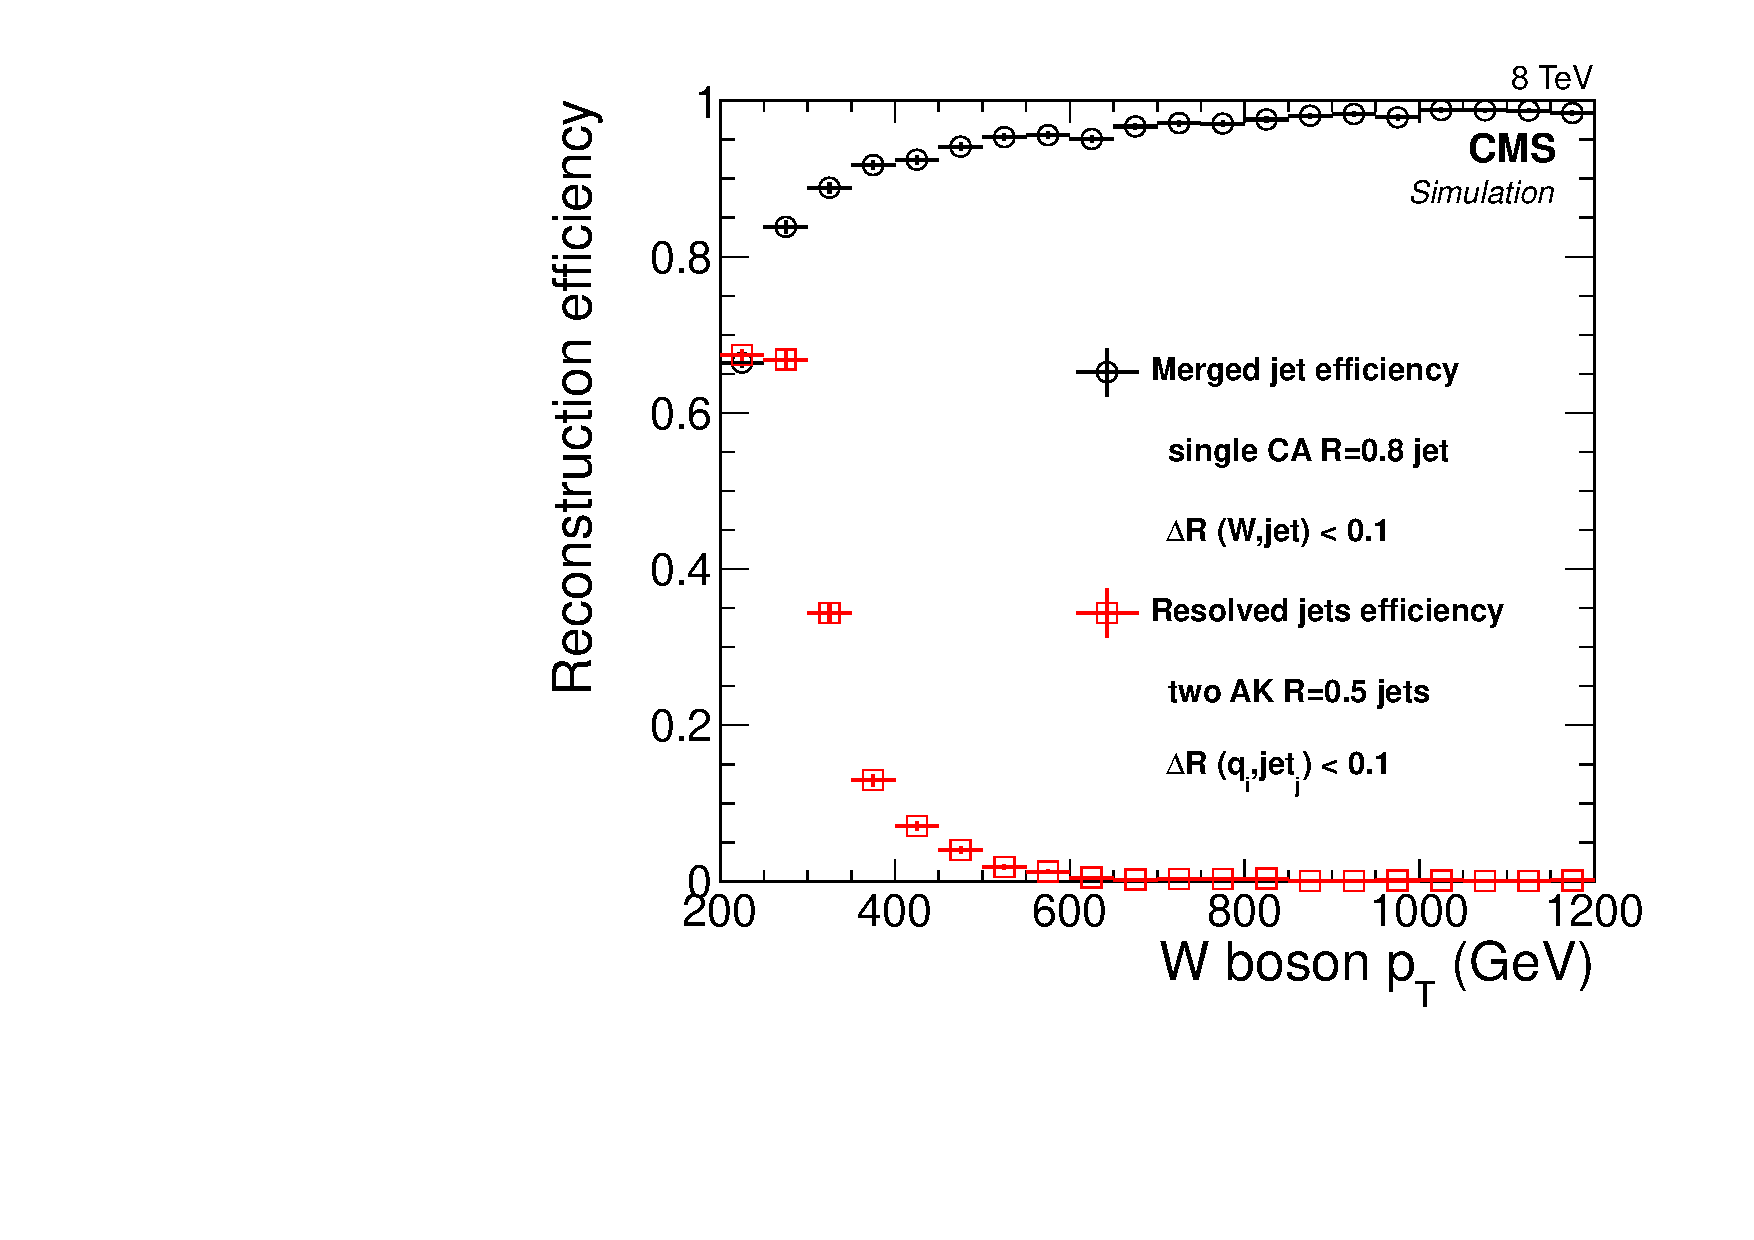
\includegraphics[width=0.7\textwidth]{figures/razor_wtag/ca8effVsPt}
  \caption{Efficiency to reconstruct a CA8 jet within $\Delta R<0.1$ of a generated $\W$ boson, and
the efficiency to reconstruct two AK5 jets within $\Delta R<0.1$ of the generated quarks from
longitudinally polarized $\W$ bosons, as a function of the $\pt$ of the $\W$
boson~\cite{Khachatryan:2014vla}. The loss in efficiency for the resolved case is clearly visible
for high $\pt$ $\W$ bosons. 
  \label{fig:boost_wtag_ca8eff}}
\end{figure}

The merged jet can be distinguished from other jets by its jet substructure, as illustrated in
Fig.~\ref{fig:boost_wtag_cartoon}. Jets originating from a $\W$ boson should have a two-prong
structure, whereas a quark/gluon-initiated jet is not expected to have this structure. 
In recent years, jet substructure techniques have seen very active developments, and many different
options are on the market~\cite{Krohn:2009th,Gallicchio:2010sw,Butterworth:2008iy,Kaplan:2008ie}.
For the razor boost analysis we will use the CMS recommendation
in terms of which techniques to use~\cite{CMS-PAS-JME-13-006,Khachatryan:2014vla}. We will employ
\textit{jet pruning} and a set of variables called \textit{N-subjettiness}. On top of these jet
substructure techniques we will also use the jet mass variable to distinguish $\W$ boson-initiated
jets
from quark/gluon-initiated jets. 
The following subsections will go through the different parts of the
$\W$ tagging definition, providing a more detailed explanation for each.

\begin{figure}
  \centering
  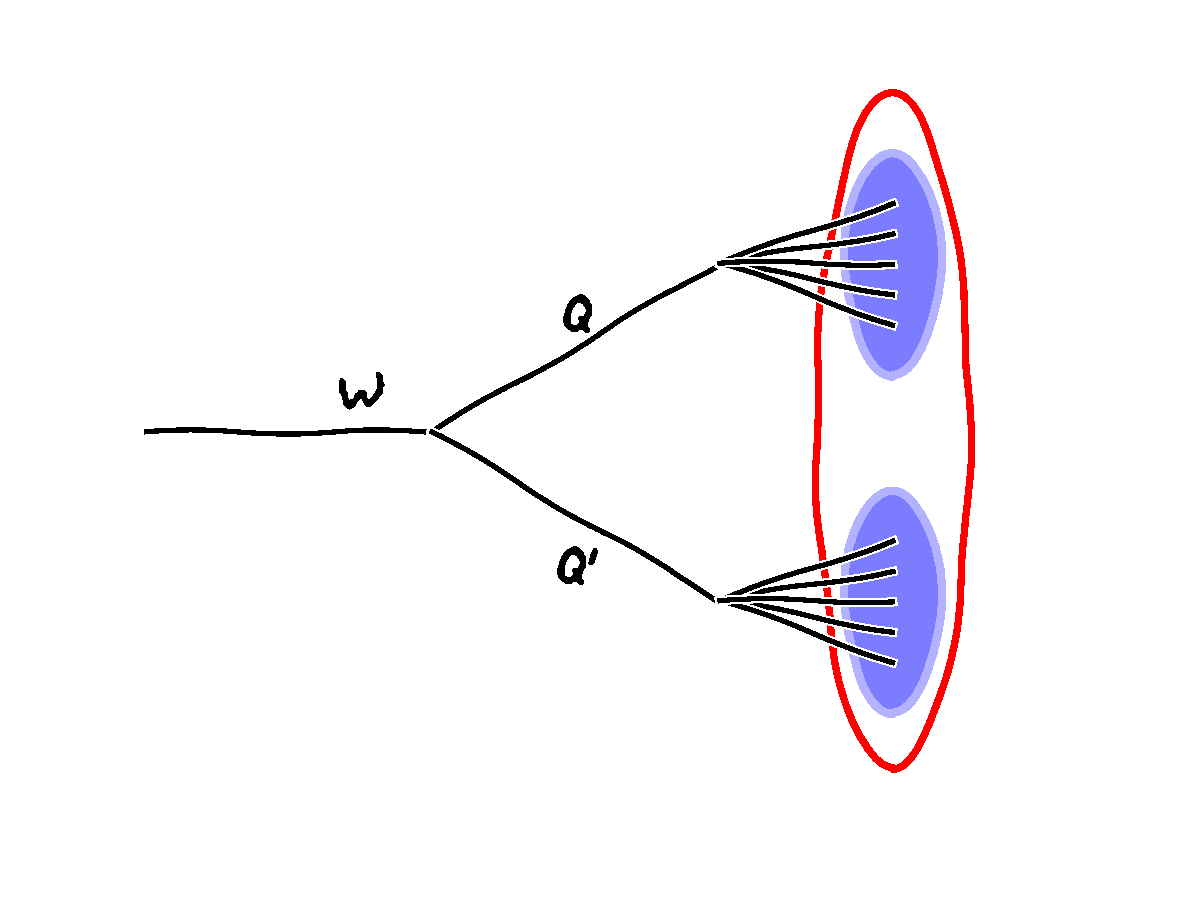
\includegraphics[width=0.48\textwidth]{figures/razor_wtag/W_subjets}
  ~
  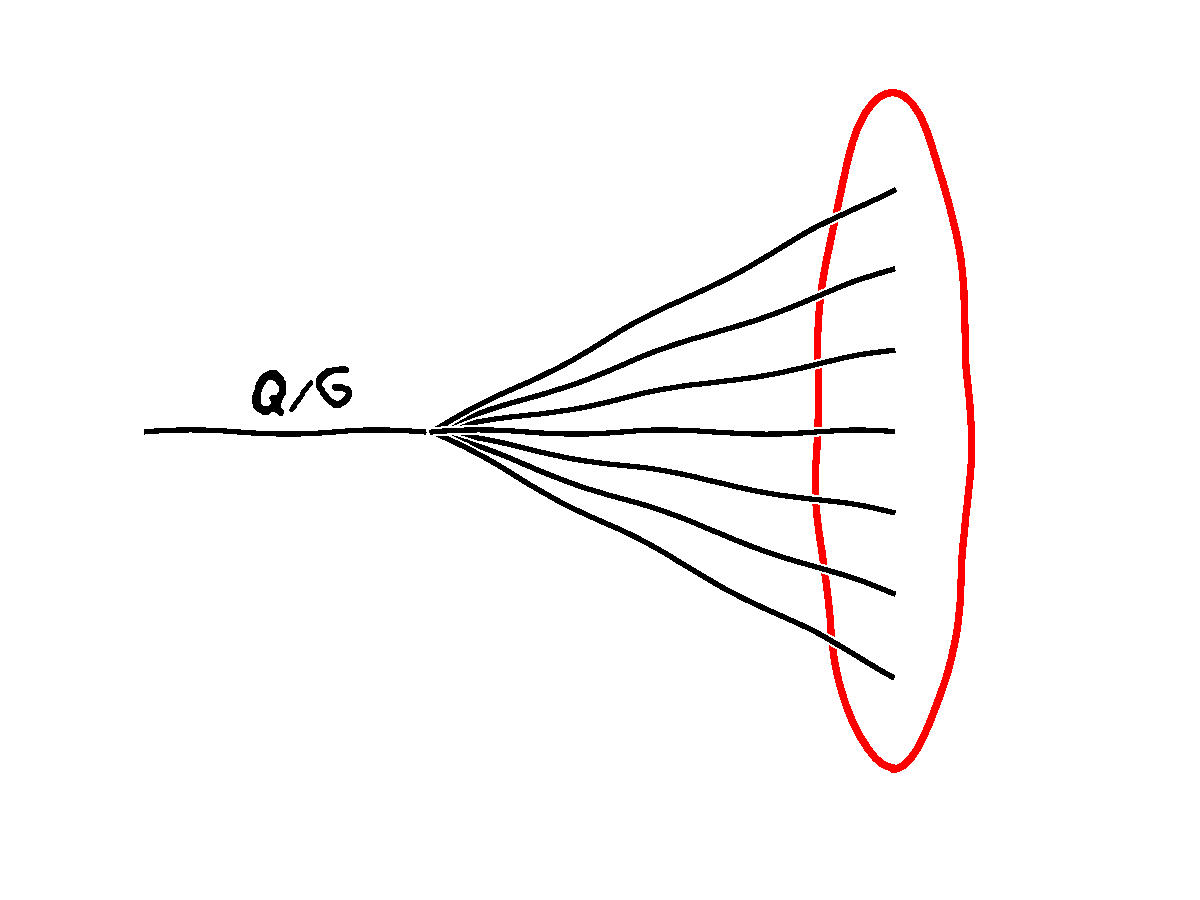
\includegraphics[width=0.48\textwidth]{figures/razor_wtag/qg_jets}
  \caption{The jet substructure of a $\W$-initiated jet differs from a quark/gluon-initiated jet.
  \label{fig:boost_wtag_cartoon}}
\end{figure}

%%%%%%%%%%%%%%%%%%%%%%%%%%%%%%%%%%%%%%%%%%%%%%%%%%%%%%%%%%%%%%%%%%%%%%%%%%%%%%%%%%%%%%%%%%%%%%%%%%%%

\subsection{Jet algorithm}

In order to identify boosted $\W$ bosons,  we will use a different jet clustering algorithm
than what is used for the standard jet definition (see Section~\ref{sec:object_jets}). 
Jets will be clustered with \textsc{FastJet 3.0.1.}~\cite{Cacciari:2011ma}, from the PF candidates,
using the Cambridge-Aachen (CA) algorithm~\cite{Dokshitzer:1997in} with a size parameter of 0.8.
Henceforth, we will call these jets \textit{CA8 jets}. 

%\begin{quote}
\begin{cajet} \theoremstyle{definition}
The Cambridge-Aachen jet algorithm is a sequental recombination algorithm that uses the
distance measure $d_{ij}$ between two constituents $i$ and $j$,
\begin{equation}
d_{ij} = \frac{\Delta R_{ij}^2}{R^2}, \label{eq:CA_distance}
\end{equation}
with $R$ the size parameter of the resulting jets, and
\begin{equation}
\Delta R_{ij}^2 = (y_i - y_j)^2 + (\phi_i - \phi_j)^2 ,
\label{eq:DeltaR_jet_algo}
\end{equation}
where $y, \phi$ are the rapidity (defined in Eq.~\ref{eq:rapidity}) and azimuthal angle. 
%The rapidity is given in terms of energy and longitudinal momentum as
%\begin{equation}
%  y = \frac{1}{2} \ln{\frac{ E + p_z }{ E - p_z }} .
%\end{equation}
The distance between constituent $i$ and the beam is given by $d_{iB} = 1$.
As is clear from the above, these distance measures only use angular information, unlike for the
$k_T$ and anti-$k_T$ algorithms, which use a $\pt$-weighted distance. 

The jet algorithm starts by computing the minimum distance $d_{ij}$, across all $i,j$. If $\min
d_{ij} < d_{iB}$, then we combine constituents $i$ and $j$ into a new constituent whose
four-momentum is the sum of the four-momenta of $i$ and $j$, and repeat the process. Otherwise, we
call $i$ a jet and remove it from the list of constituents to be clustered. Again, the process is
repeated with the remaining constituents, until none remain.
\end{cajet}
%\end{quote}

Jet energy corrections for these CA8 jets are derived from the standard anti-$k_\textrm{T}$ jets
with size parameter $R=0.7$. Simulations show that the corrections are valid for CA8 jets and
have an additional uncertainty no greater than 2\%~\cite{CMS-PAS-JME-13-007}.  
% seems like no better reference is available for this...

%%%%%%%%%%%%%%%%%%%%%%%%%%%%%%%%%%%%%%%%%%%%%%%%%%%%%%%%%%%%%%%%%%%%%%%%%%%%%%%%%%%%%%%%%%%%%%%%%%%%

\subsection{Jet pruning}

Jet pruning~\cite{Ellis:2009su,Ellis:2009me} is a particular kind of jet grooming. Jet grooming
techniques are designed to reduce the impact of contributions from the underlying event (UE), pileup
(PU), and low-\pt gluon radiation. These kinds of contributions to jets are typically soft and
diffuse, and increase the jet energy proportional to the jet area. Grooming techniques reduce the
jet area without affecting the core components. This means that the resulting jets are less
sensitive to these soft contributions, but still reflect the kinematics of the original, hard
process.


During jet pruning the constituents of the jet are reclustered through the CA algorithm, using the
same distance parameter as used for the original jets (here $R=0.8$), but with additional conditions
beyond those of the standard algorithm.
In particular, the softer and larger-angle of the two particles $i$ and $j$ to be merged is removed
when the following conditions are satisfied:
\begin{align}
  z_{ij} &= \frac{\min( \pt^i , \pt^j )}{\pt^i + \pt^j} < z_{\textrm{cut}}, \\
  \Delta R_{ij} &> D_{\textrm{cut}} \equiv \alpha \frac{m_J}{\pt} ,
\end{align}
where $m_J$ and $\pt$ are the mass and transverse momentum of the originally-clustered jet, $\Delta
R_{ij}$ is defined as in Eq.~\ref{eq:DeltaR_jet_algo}, and
$z_\textrm{cut}$ and $\alpha$ are parameters of the algorithm, chosen to be 0.1 and 0.5,
respectively~\cite{Chatrchyan:2013vbb}. 

The resulting pruned jet is used as further input to our $\W$ boson tagger. For the $\W$ decay
products to be collimated, we need a large transverse momentum. We will therefore require that the
pruned jets have $\pt > 200\GeV$. 
Because of the reduction of the effect of UE and PU, the jet mass variable as computed from the
constituents of the jet after jet pruning has a much better behavior than if it was computed from
the unpruned jets, see Fig.~\ref{fig:wtag_jet_pruning}. Jet pruning shifts the jet mass of QCD jets
to smaller values, while maintaining the jet mass for $\W$ jets close to the $\W$ boson mass.

We will make the requirement that the pruned jet mass is consistent with the $\W$ boson mass,
\begin{equation}
  70 < m_{\textrm{pruned jet}} < 100 \GeV .
\end{equation}
Here, we have deviated from the standard interval used in CMS, starting at 60\GeV, as we found that
for our
kinematical region and signal topology we achieve better signal to background discrimination when
increasing the lower cut value to 70\GeV. 
%This provides good boosted $\W$ jet to quark/gluon jet discrimination. 

\begin{figure}
  \centering
  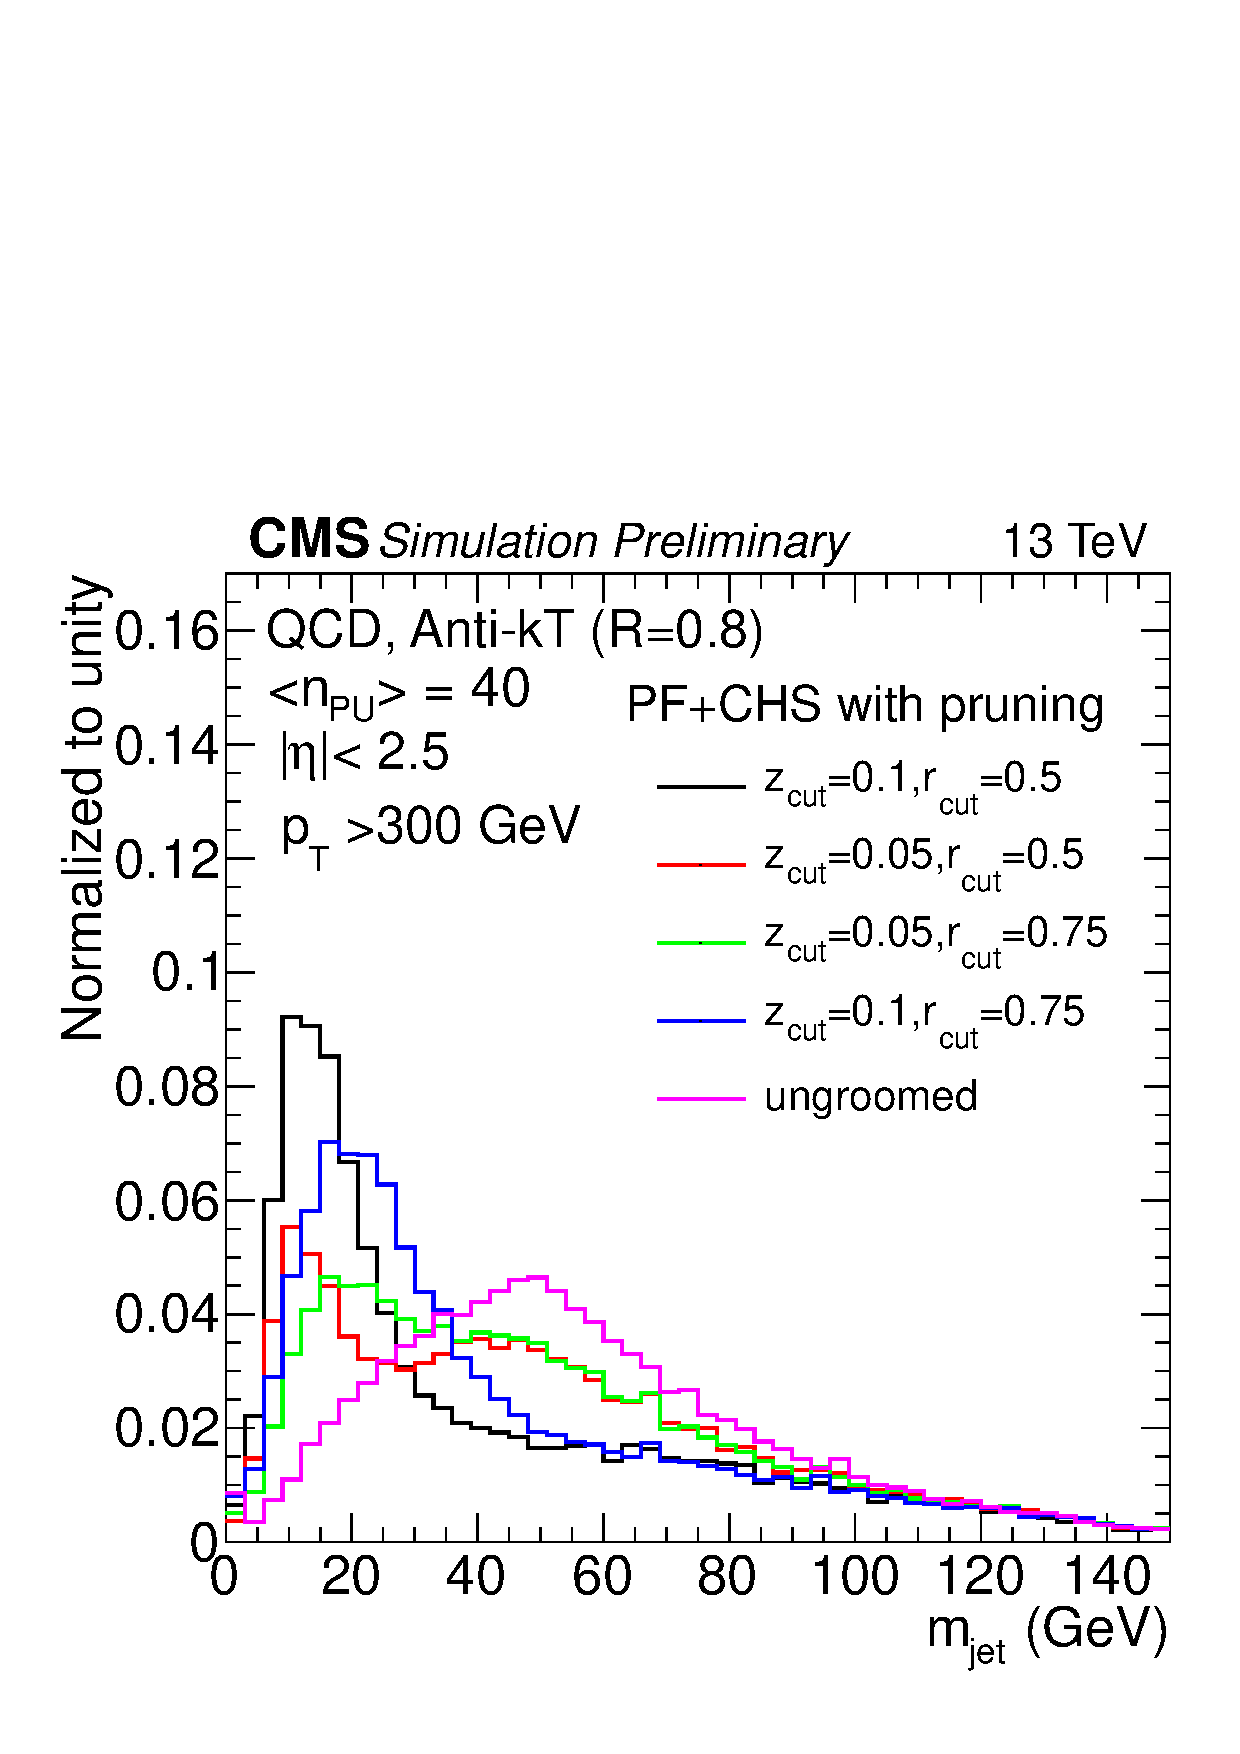
\includegraphics[width=0.6\textwidth]{figures/razor_wtag/1DPFCHS_PR_QCD}
  \caption{Jet mass distribution of QCD jets with $\pt(\textrm{gen}) > 300 \GeV$ for jet pruning
with different parameters, starting from PF jets with charge-hadron subtraction applied. The fully
ungroomed mass distribution is also shown for comparison~\cite{CMS-PAS-JME-14-001}. 
  \label{fig:wtag_jet_pruning}}
\end{figure}

%%%%%%%%%%%%%%%%%%%%%%%%%%%%%%%%%%%%%%%%%%%%%%%%%%%%%%%%%%%%%%%%%%%%%%%%%%%%%%%%%%%%%%%%%%%%%%%%%%%%

\subsection{N-subjettiness}

Requiring the jet mass to be consistent with the $\W$ boson mass already results in a good
discrimination between $\W$ boson and quark/gluon-initiated jets. We can however still do better. A
boosted QCD jet with a mass around 80\GeV usually originates from a single hard parton and acquires
mass through large angle soft splittings. The energy pattern for this process will differ from the
two-prong pattern that is found in boosted $\W$ jets.  
The set of N-subjettiness observables $\tau_N$~\cite{Thaler:2010tr} aims to exploit this difference
in expected energy flow to differentiate between $\W$ boson and quark/gluon-initiated jets by
counting the number of hard lobes of energy within a jet.

N-subjettiness is computed under the assumption that the jet has N subjets, and is the
$\pt$-weighted $\Delta R$ distance between each jet constituent and its nearest subjet axis:
\begin{equation}
\tau_N = \frac{1}{R_0 \sum_{k} p_{T, k}} \sum_k p_{T, k} \min (\Delta R_{1,k}, \Delta R_{2,k}, ...
\Delta R_{N,k}),
\end{equation}
where $R_0$ is the original jet distance parameter (0.8 in our case) and $k$ runs over all
constituent particles of the jet. 
The subjet axes are obtained by running the exclusive $k_T$
algorithm~\cite{Ellis:1993tq,Catani:1993hr} using \textsc{FastJet}. 
The exclusive $k_T$ algorithm differs from the inclusive version in two ways: if at a given
clustering step $d_{iB} < \min_j d_{ij}$, then constituent $i$ is discarded, rather than added to
the jet collection; and the clustering stops when the desired number of jets (N) is reached. 
The resulting axes can be further optimized to minimize the N-subjettiness value. In accordance to
the CMS recommendation, we use a “one-pass” optimization of the exclusive $k_T$
axes~\cite{nsubjettiness_fastjet}.

The variables $\tau_N$ quantify the consistency of the jet having N or fewer subjets. They have a
small value (close to 0) if the original jet is consistent with having N or fewer subjets, because
almost every jet constituent will be close in $\Delta R$ to its own true subjet. 
As we are interested in discriminating boosted $\W$ bosons, with two subjets, from quark/gluon
jets, which have a single subjet, we will use the variables $\tau_2$ and $\tau_1$, as obtained
from the unpruned CA8 jets. To ensure that the N-subjettiness ratio as computed from the unpruned
jet collection is assigned to the correct pruned jet, we find the highest \pt unpruned jet that is
within $\Delta R = 0.7$ of the considered pruned jet.  
It has been shown that the ratio of the $\tau_N$ variables are better discriminitors than the
separate variables. We will thus require that the ratio $\tau_2 / \tau_1$ is small. The $\tau_2 /
\tau_1$ distribution for highly boosted and longitudinally polarized $\W$ bosons and for inclusive
QCD jets is shown in Fig.~\ref{fig:boost_wtag_tau2tau1}. 

\begin{figure}[htpb]
  \centering
  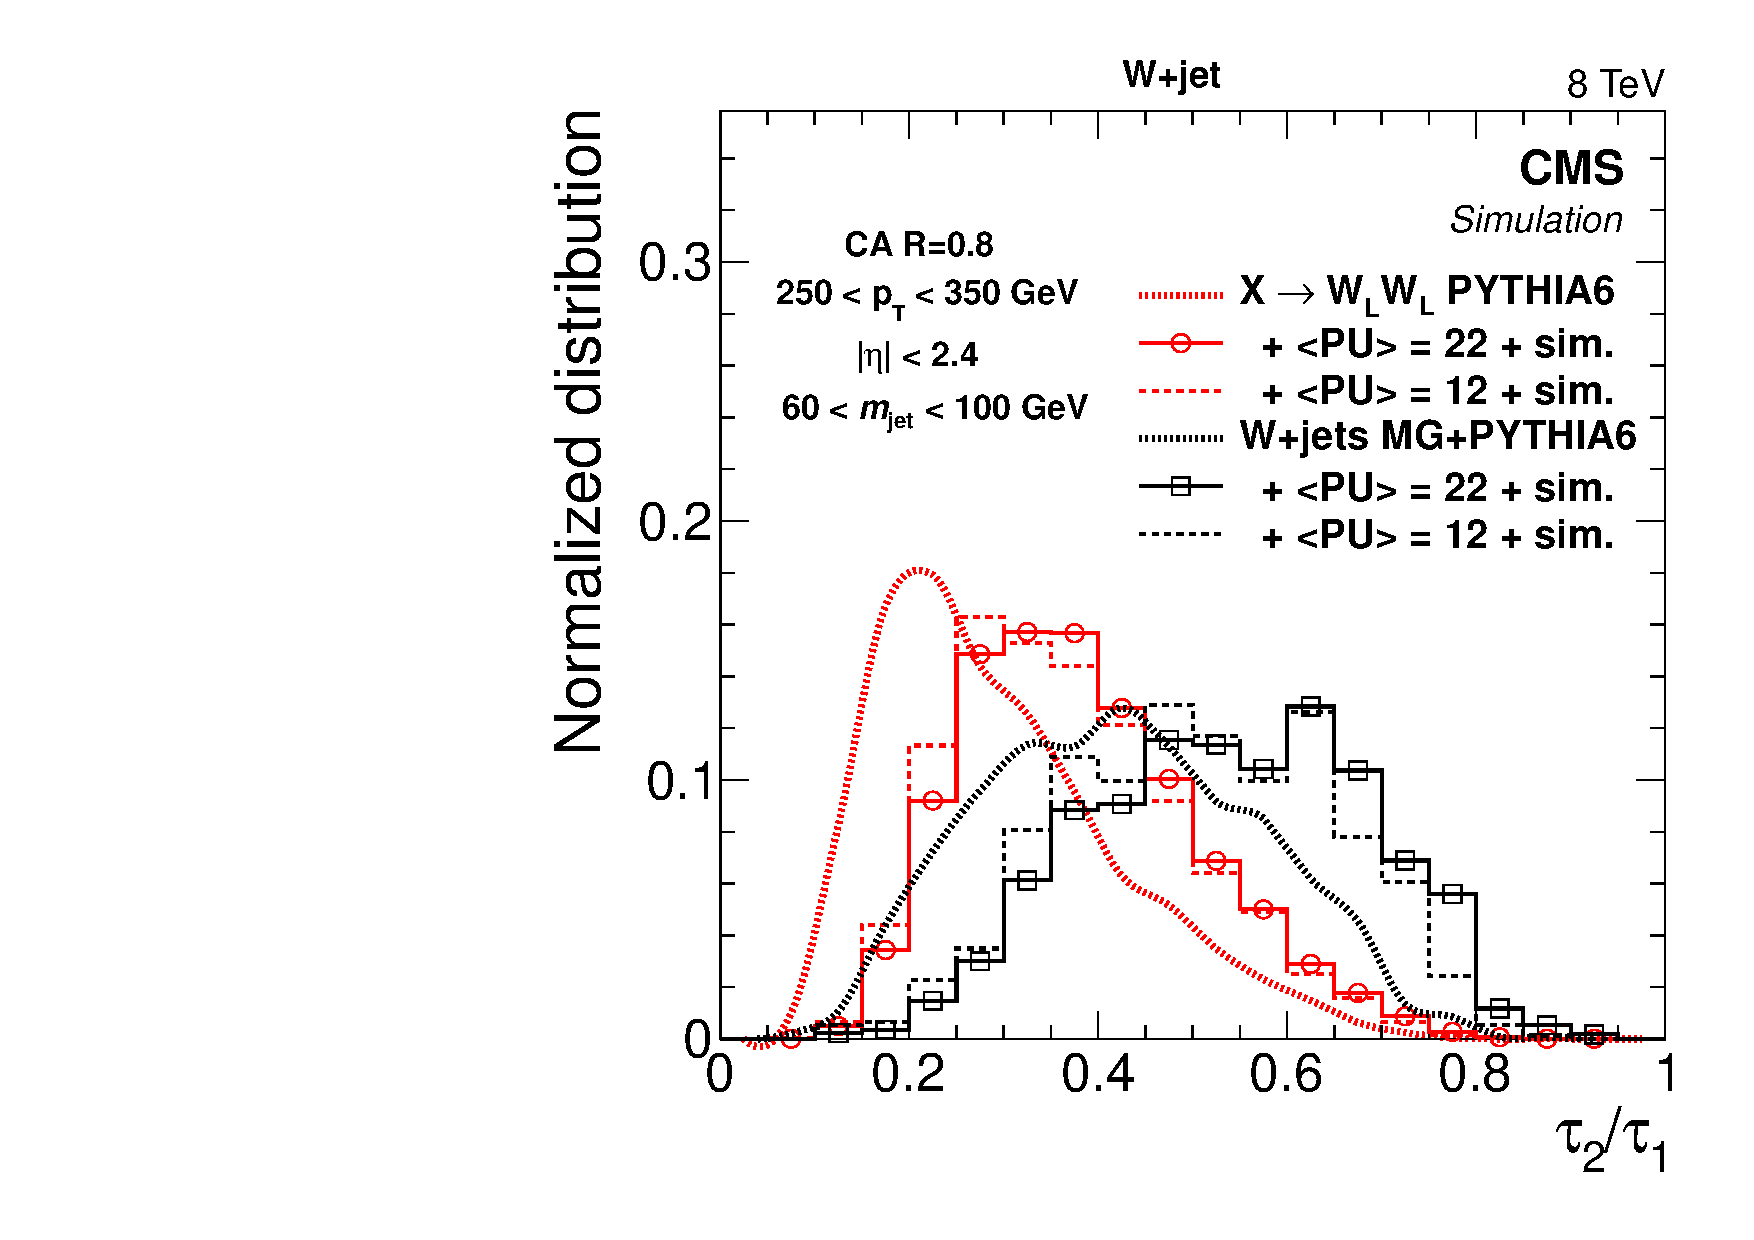
\includegraphics[width=0.7\textwidth]{figures/razor_wtag/tau2tau1_afterMass}
  \caption{Distributions of the N-subjettiness ratio $\tau_2 / \tau_1$ in simulated samples of
highly boosted and longitudinally polarized $\W$ bosons and inclusive QCD jets expected in the
$\W$+jet topology (i.e. with leptonically decaying $\W$ bosons recoiling off a hard jet). 
The distribution is shown after a selection on the pruned jet mass of $60 < m_{\textrm{pruned jet}}
< 100 \GeV$. Note that this is slightly different from what is applied in the razor boost analysis.
Thick dashed lines represent the generator predictions without pileup interactions and without CMS
detector simulation. The histograms are the expected distributions after full CMS simulation with
pileup corresponding to an average number of 12 and 22 interactions~\cite{Khachatryan:2014vla}. 
  \label{fig:boost_wtag_tau2tau1}}
\end{figure}


%%%%%%%%%%%%%%%%%%%%%%%%%%%%%%%%%%%%%%%%%%%%%%%%%%%%%%%%%%%%%%%%%%%%%%%%%%%%%%%%%%%%%%%%%%%%%%%%%%%%

\subsection{\texorpdfstring{$\W$}{W} boson tagging definitions}

In the razor boost analysis we will emply a boosted $\W$ boson tagger, utilizing the techniques
outlined in the previous sections, to identify events that are consistent with the presence of a
high \pt, hadronically decaying $\W$ boson. 
A given pruned CA8 jet is $\W$ tagged if it has $\pt > 200\GeV$, $|\eta|<2.4$, $70 < m_\textrm{jet}
< 100\GeV$, and the corresponding unpruned jet satisfies $\tau_2 / \tau_1 < 0.5$.
This definition is the same as was used previously in a search for massive resonances in dijet
systems containing jets tagged as a W or Z boson~\cite{EXO-12-024,EXO-13-009}. 
The precise definition of this $\W$ boson tagger is summarized in Table~\ref{tab:Wtag_definition}.

As explained in Section~\ref{sec:boost_strategy}, we will use three control regions to select data
samples enriched in QCD multijet, $t\bar{t}$, and $\W(\rightarrow l \nu)+$jets, in order to help
model the SM backgrounds. QCD multijet and leptonically decaying $\W$+jets events are not expected
to have jets with a two-prong substructure. Therefore, our $\W$ boson tagging definition will not be
very efficient in selecting these processes. To remedy this, we slightly modify our $\W$ tagger. 
We define $\W$ boson \textit{anti-tagged} jets by taking the complement of the $\tau_2 / \tau_1$
requirement, and define $\W$ boson \textit{mass-tagged} jets by dropping that requirement all
together. 
These definitions allow a more efficient selection of background processes, while remaining in a
similar kinematic regime. How these taggers will be used exactly will be explained in
Section~\ref{sec:boost_control_selection}. A summary of their definition can be found in
Table~\ref{tab:Wtag_definition} as well. 

\begin{table}[htdp]
\caption{Boosted $\W$ tagging definitions. The input jet collection is either the pruned or unpruned
CA8 jet collection with charged-hadron subtraction applied. }
\vspace{1ex}
\centering
\begin{tabular}{l c c c}
\toprule
& $\W$ tagging & $\W$ anti-tagging & $\W$ mass-tagging  \\
\midrule
\multirow{3}{*}{Pruned} & $\pt > 200$  & $\pt > 200$  & $\pt > 200$\\
& $|\eta| < 2.4$ & $|\eta| < 2.4$ & $|\eta| < 2.4$\\
& $70 < m_{\textrm{jet}}< 100$ & $70 < m_{\textrm{jet}}< 100$ & $70 < m_{\textrm{jet}}< 100$\\
\midrule
Unpruned & $\tau_2 / \tau_1 < 0.5$ & $\tau_2 / \tau_1 \geq 0.5$ & -\\
\bottomrule
\end{tabular}
\label{tab:Wtag_definition}
\end{table}

%%%%%%%%%%%%%%%%%%%%%%%%%%%%%%%%%%%%%%%%%%%%%%%%%%%%%%%%%%%%%%%%%%%%%%%%%%%

\subsection{\texorpdfstring{$\W$}{W} boson tagging scale factors \label{sec:wtag_scale_factor}}

It has been observed by previous CMS analyses that the $\W$ boson tagging efficiency is not the same
in data and in simulation. The distributions that are at the root of this disagreement are shown on
Fig.~\ref{fig:boost_wtag_data_sim}. 
To account for the discrepancies, we need to derive data/MC scale factors and associated
uncertainties corresponding to each of the $\W$ boson tagging, mass-tagging and anti-tagging
definitions listed in Table~\ref{tab:Wtag_definition}. These scale factors are not
process-independent. They will be different for processes that include hadronically decaying $\W$
bosons, such as $t\bar{t}$ or the signal, compared to processes which do not have $\W$ bosons in
their final state, such as QCD multijet production. For processes without real hadronically
decaying $\W$ bosons, any tagged jet is necessarily a misidentified, or \textit{fake}, $\W$ boson
tag. For those processes we will speak of the $\W$ boson tagging fake rate scale factors, where the
fake rate is defined as the probability to tag, with one of the used W tagging definitions, a jet
not coming from a hadronically decaying $\W$ boson. 
One last consideration concerns the signal simulation. As the signal is simulated with FastSim, we
need an additional scale factor to correct for differences in the modelling of the $\W$ tagger
between FastSim and FullSim. 
In the following subsections every scale factor will be listed in more detail, including how it was
derived and how it will be used in the analysis. 

\begin{figure}[htpb]
  \centering
  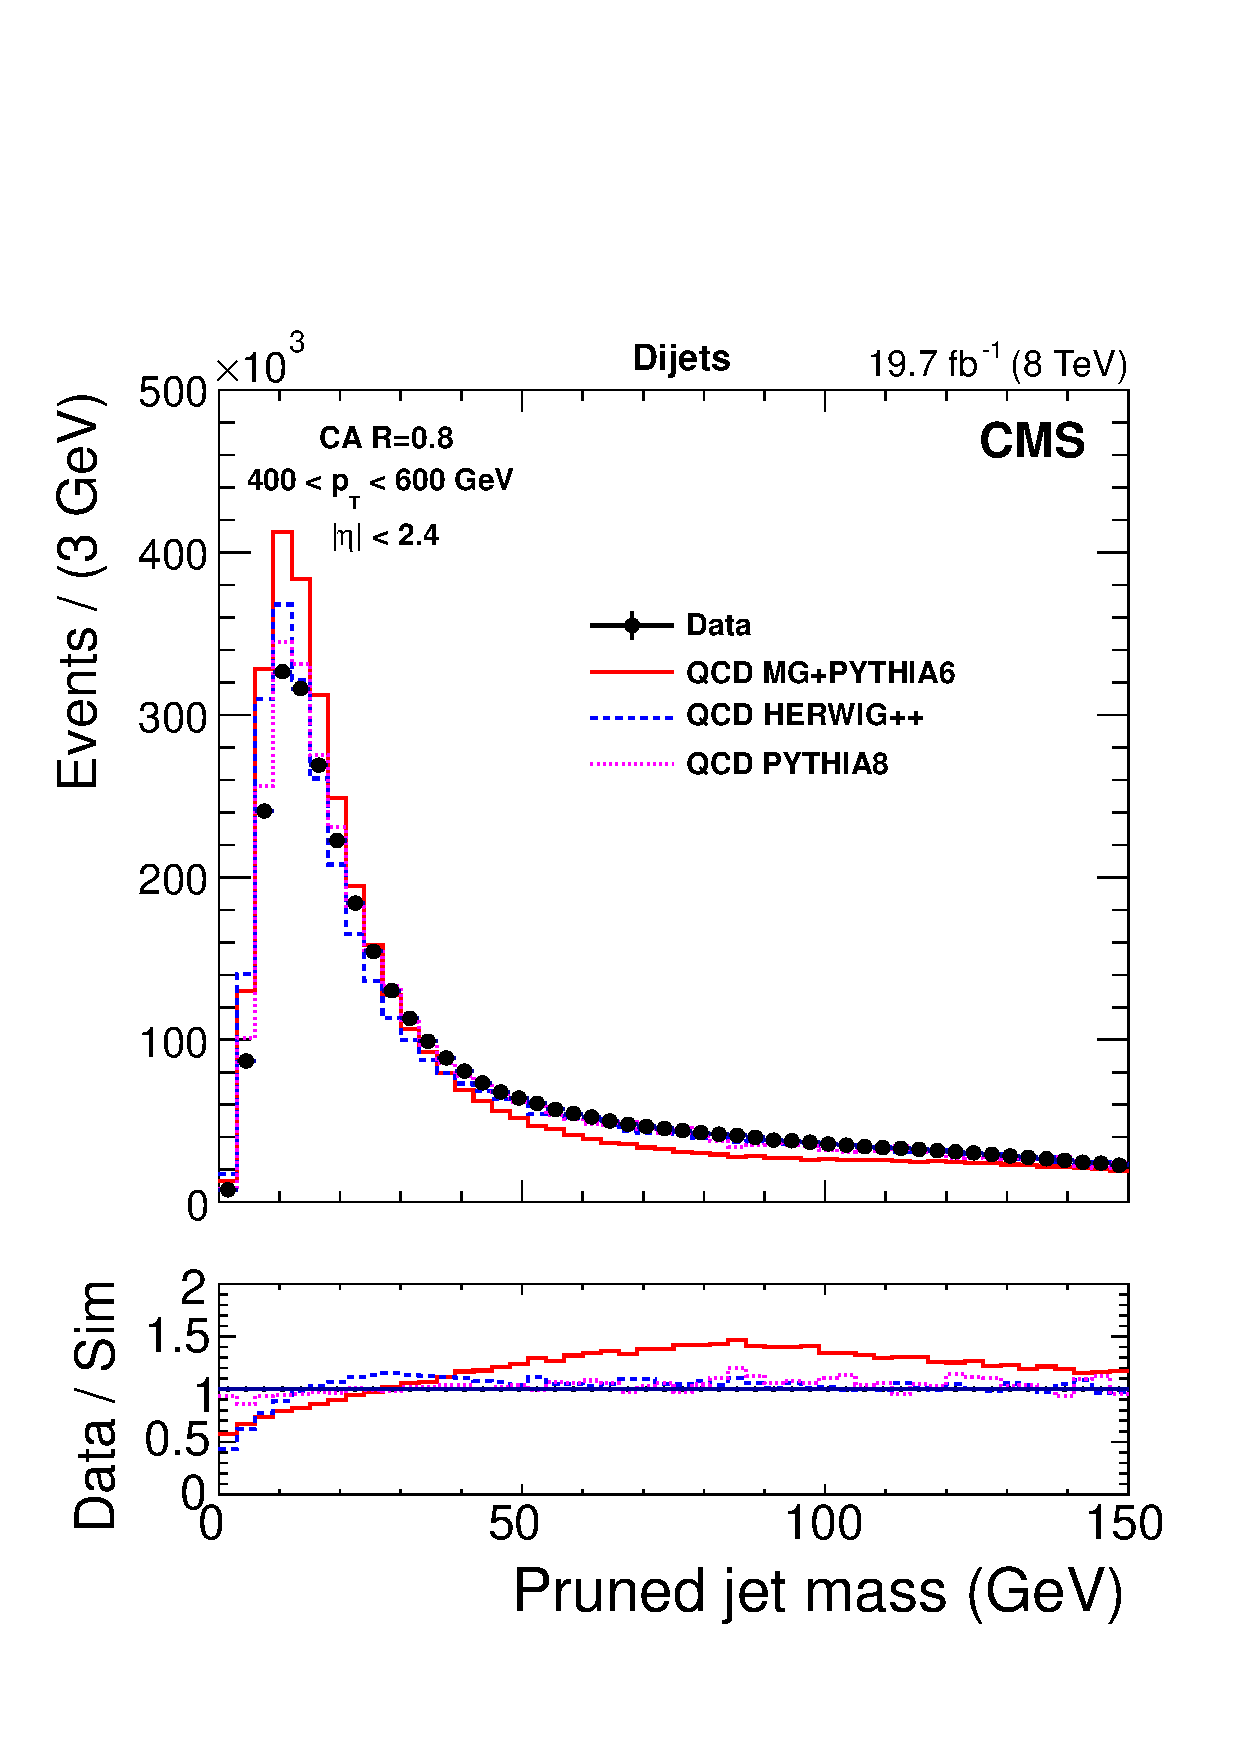
\includegraphics[width=0.48\textwidth]{figures/razor_wtag/substructure_pas_mass_2}
  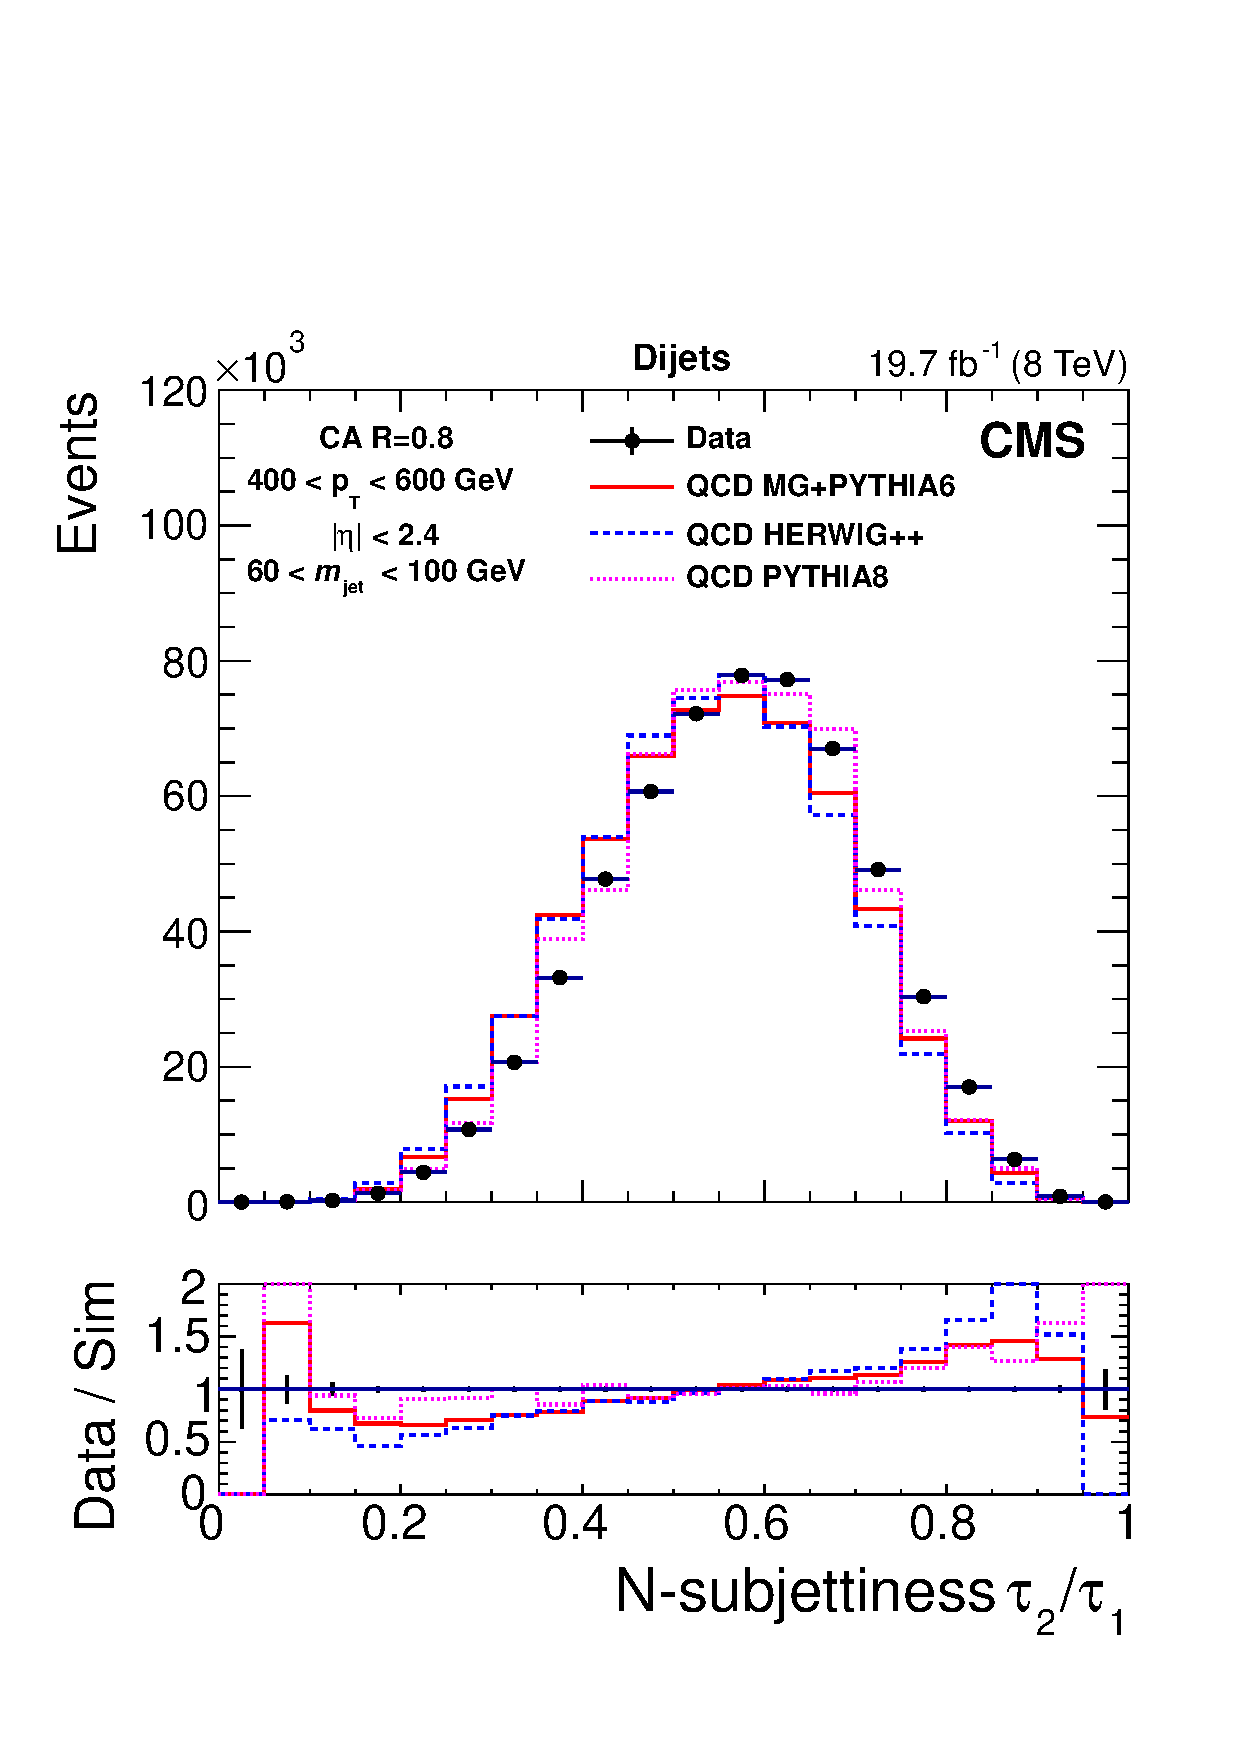
\includegraphics[width=0.48\textwidth]{figures/razor_wtag/substructure_pas_tau21_aftermass_2}
  \caption{Pruned jet mass (left) and N-subjettiness ratio $\tau_2/\tau_1$ (right) distributions 
  in data and simulation for dijet events. MG denotes the \MADGRAPH generator, and the option used
  for the razor boost analysis. Below each figure the relative deviations are plotted between data
  and simulation~\cite{Khachatryan:2014vla}. 
  \label{fig:boost_wtag_data_sim}}  
\end{figure}

%% ---------------------------------------------------------------------------------------------

\subsubsection{\texorpdfstring{$\W$}{W} boson tag efficiency scale factor \label{sec:wtag_eff_sf}}

The $\W$ boson tag efficiency scale factor will be used to correct processes with real
hadronically decaying $\W$ bosons. For the backgrounds this is mainly for the $t\bar{t}$ process,
but also single top and $t\bar{t}$ in association with a $\W$ or $\cPZ$ boson are considered. This
scale factor is of course also used for the signal processes. 

The $\W$ boson tag efficiency scale factor is only applied to the simulation in the $S$ and $T$
region, see Sections~\ref{sec:boost_signal_selection} and \ref{sec:boost_T_region}, as those are the
selections that utilize the $\W$ tagging definition. It is also only applied to events for which
the $\W$ boson tagged jet is matched (within a cone of $\Delta R = 0.8$) to a generator level
hadronically decaying $\W$ boson. In case no match was found, we apply the $\W$ boson tag fake rate
scale factor. 

As we use the same $\W$ boson tagging definition as was used for the EXO-12-024
paper~\cite{EXO-12-024}, we can directly apply the scale factor that was derived for that study. The
method used to obtain the scale factor is outlined in Ref.~\cite{CMS-PAS-JME-13-006}. 
The $\W$ boson tag efficiency scale factor $SF_{\textrm{Wtag}}$ is given by
\begin{equation}
SF_{\textrm{Wtag}} = 0.86 \pm 0.07 .
\end{equation}

%% ---------------------------------------------------------------------------------------------

\subsubsection{\texorpdfstring{$\W$}{W} boson tag efficiency FullSim/FastSim scale factor
\label{sec:wtag_eff_fastfull_sf}}

For our signal samples, which are produced with FastSim, we have derived an additional $\W$ tag
efficiency FullSim/FastSim scale factor, $SF_{\textrm{Full/Fast}}$, which is a function of the \pt
of the CA8 jet. This scale factor corrects for the different modelling of jets, jet
substructure, et cetera, in FastSim with respect to FullSim. The product of $SF_{\textrm{Wtag}}$ and
$SF_{\textrm{Full/Fast}}$ will be applied to the signal simulation. 

To compute the $\W$ boson tag efficiency FullSim/FastSim scale factor we use a sample of $t\bar{t}$
events simulated with both FullSim and FastSim. 
A FastSim versus FullSim comparison of the distributions of the pruned jet mass, the N-subjettiness
variables $\tau_1$, $\tau_2$ and their ratio $\tau_2/\tau_1$, both before and after requiring the
jets to satisfy the pruned jet mass window, is shown in
Figs.~\ref{fig:FastFull_jmass}-\ref{fig:FastFull_tau21}. It is clear that the agreement is not
perfect. The $\tau_2/\tau_1$ distribution for Fastsim is shifted with respect to FullSim. This
disagreement will then of course be translated into the efficiencies, and thus the need for a scale
factor arises. 

\begin{figure}[htpb]
\centering
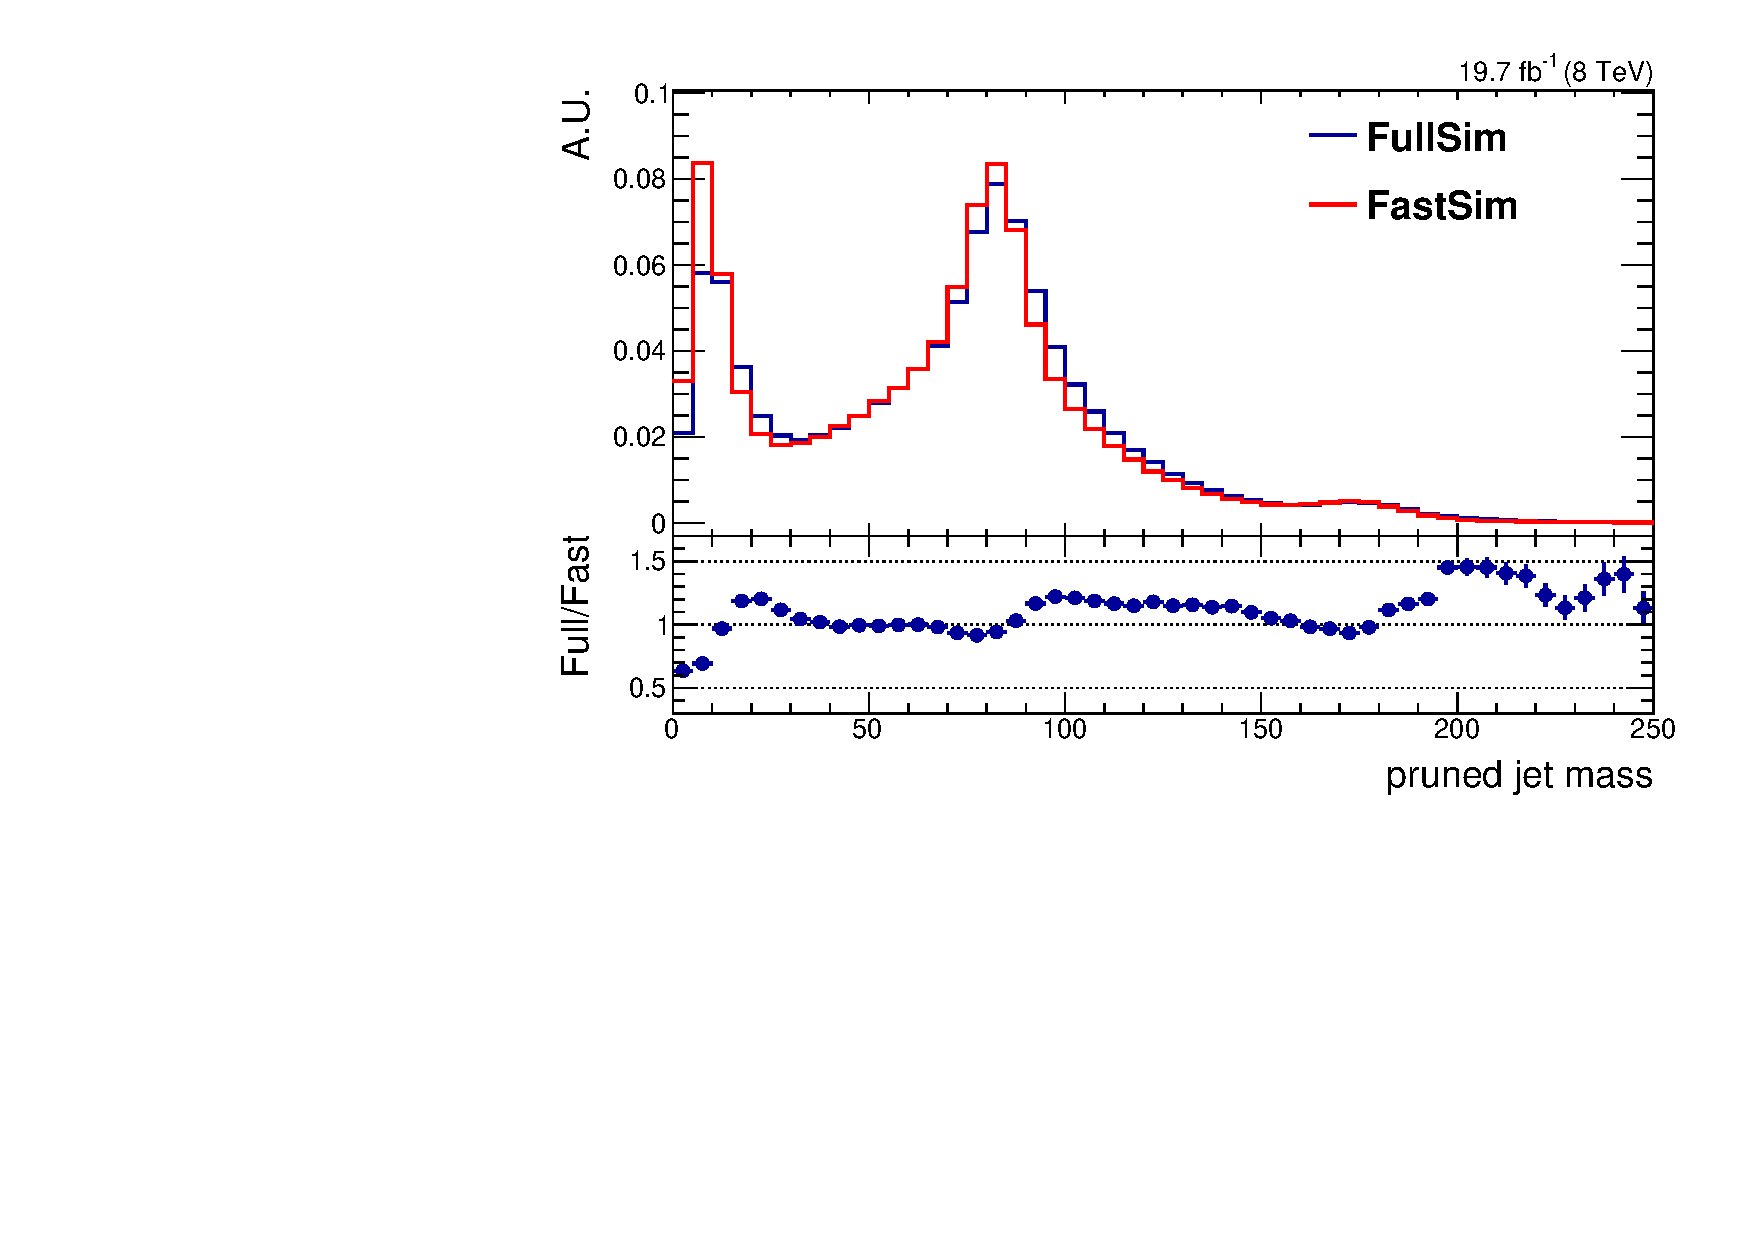
\includegraphics[width=0.7\textwidth]{figures/razor_wtag/FastFull_comparison_TTJets_jmass}
\caption{Pruned jet mass distribution for FastSim and FullSim $t\bar{t}$. 
\label{fig:FastFull_jmass}}
\end{figure}

\begin{figure}[htpb]
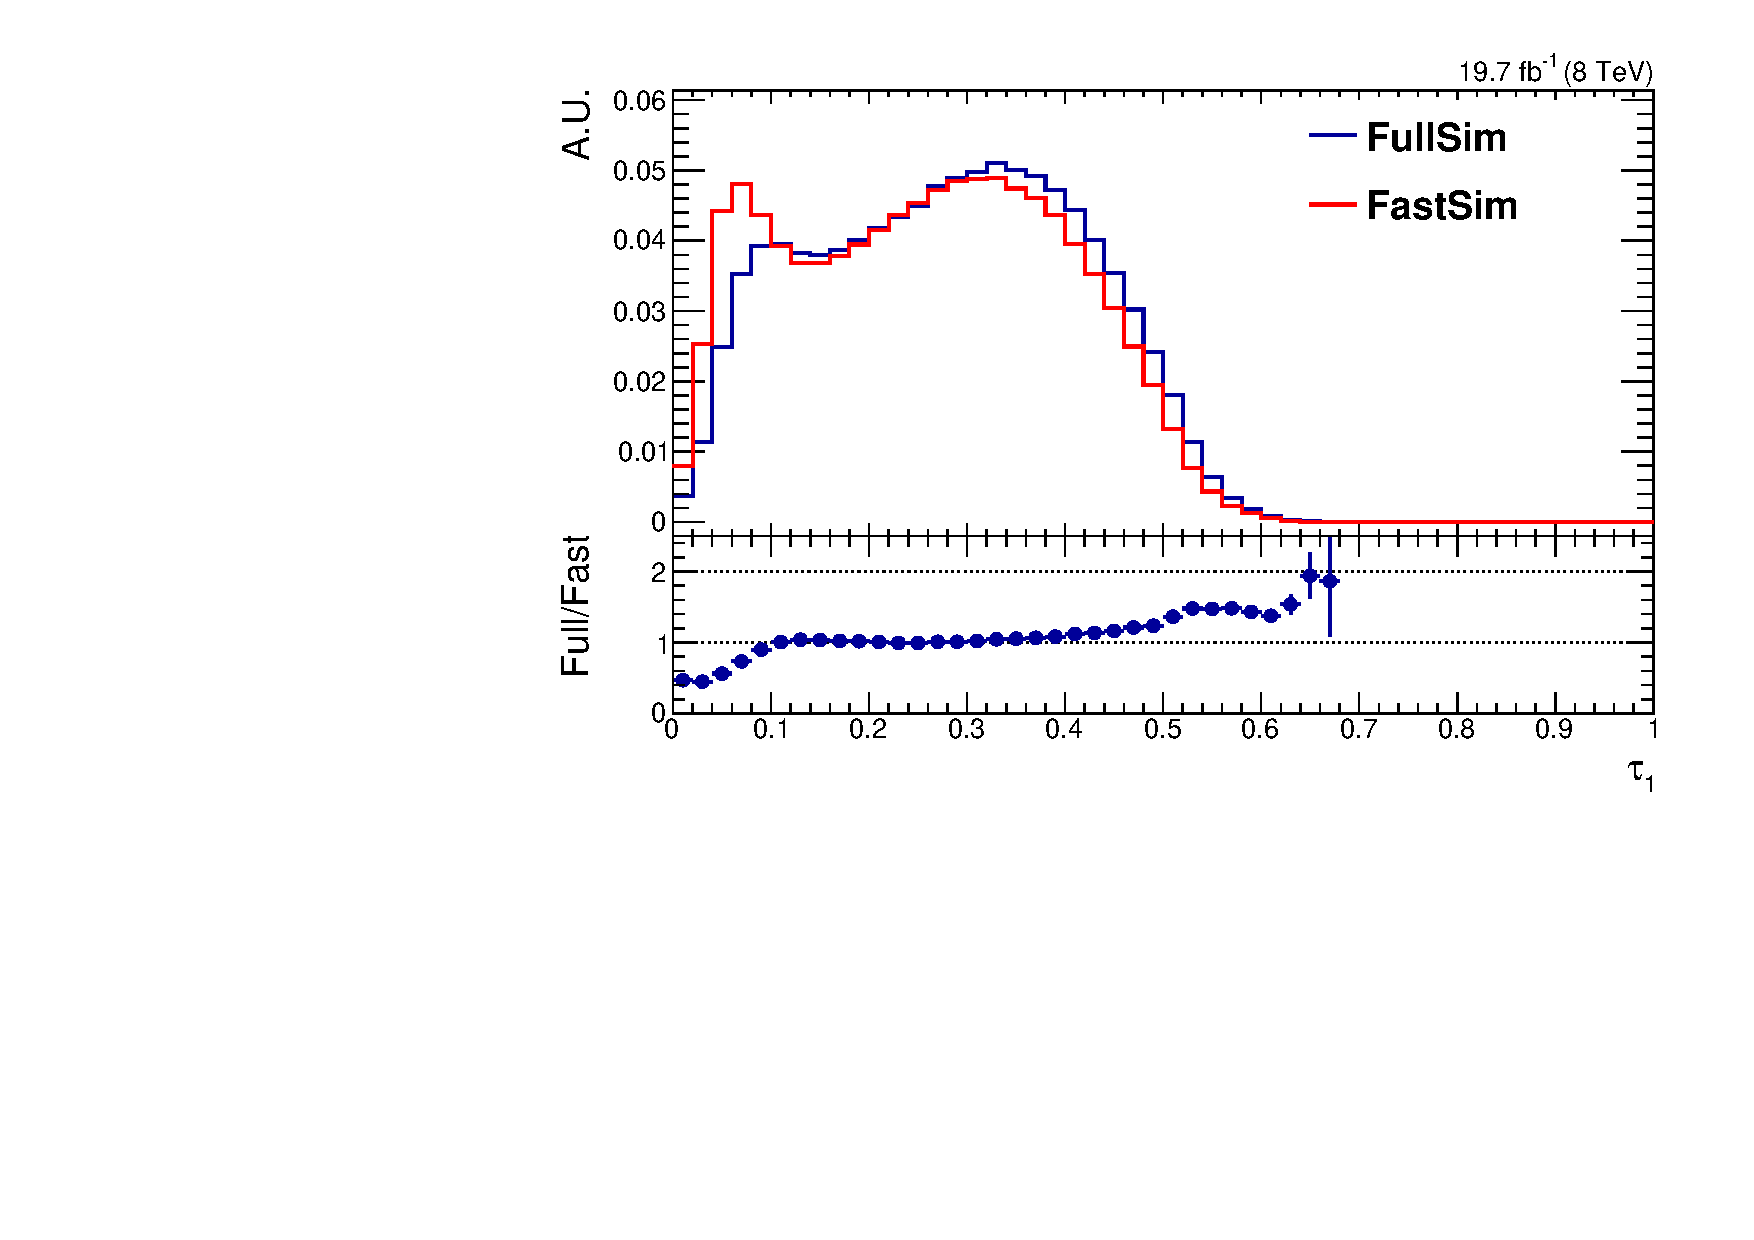
\includegraphics[width=0.49\textwidth]{figures/razor_wtag/FastFull_comparison_TTJets_tau1}
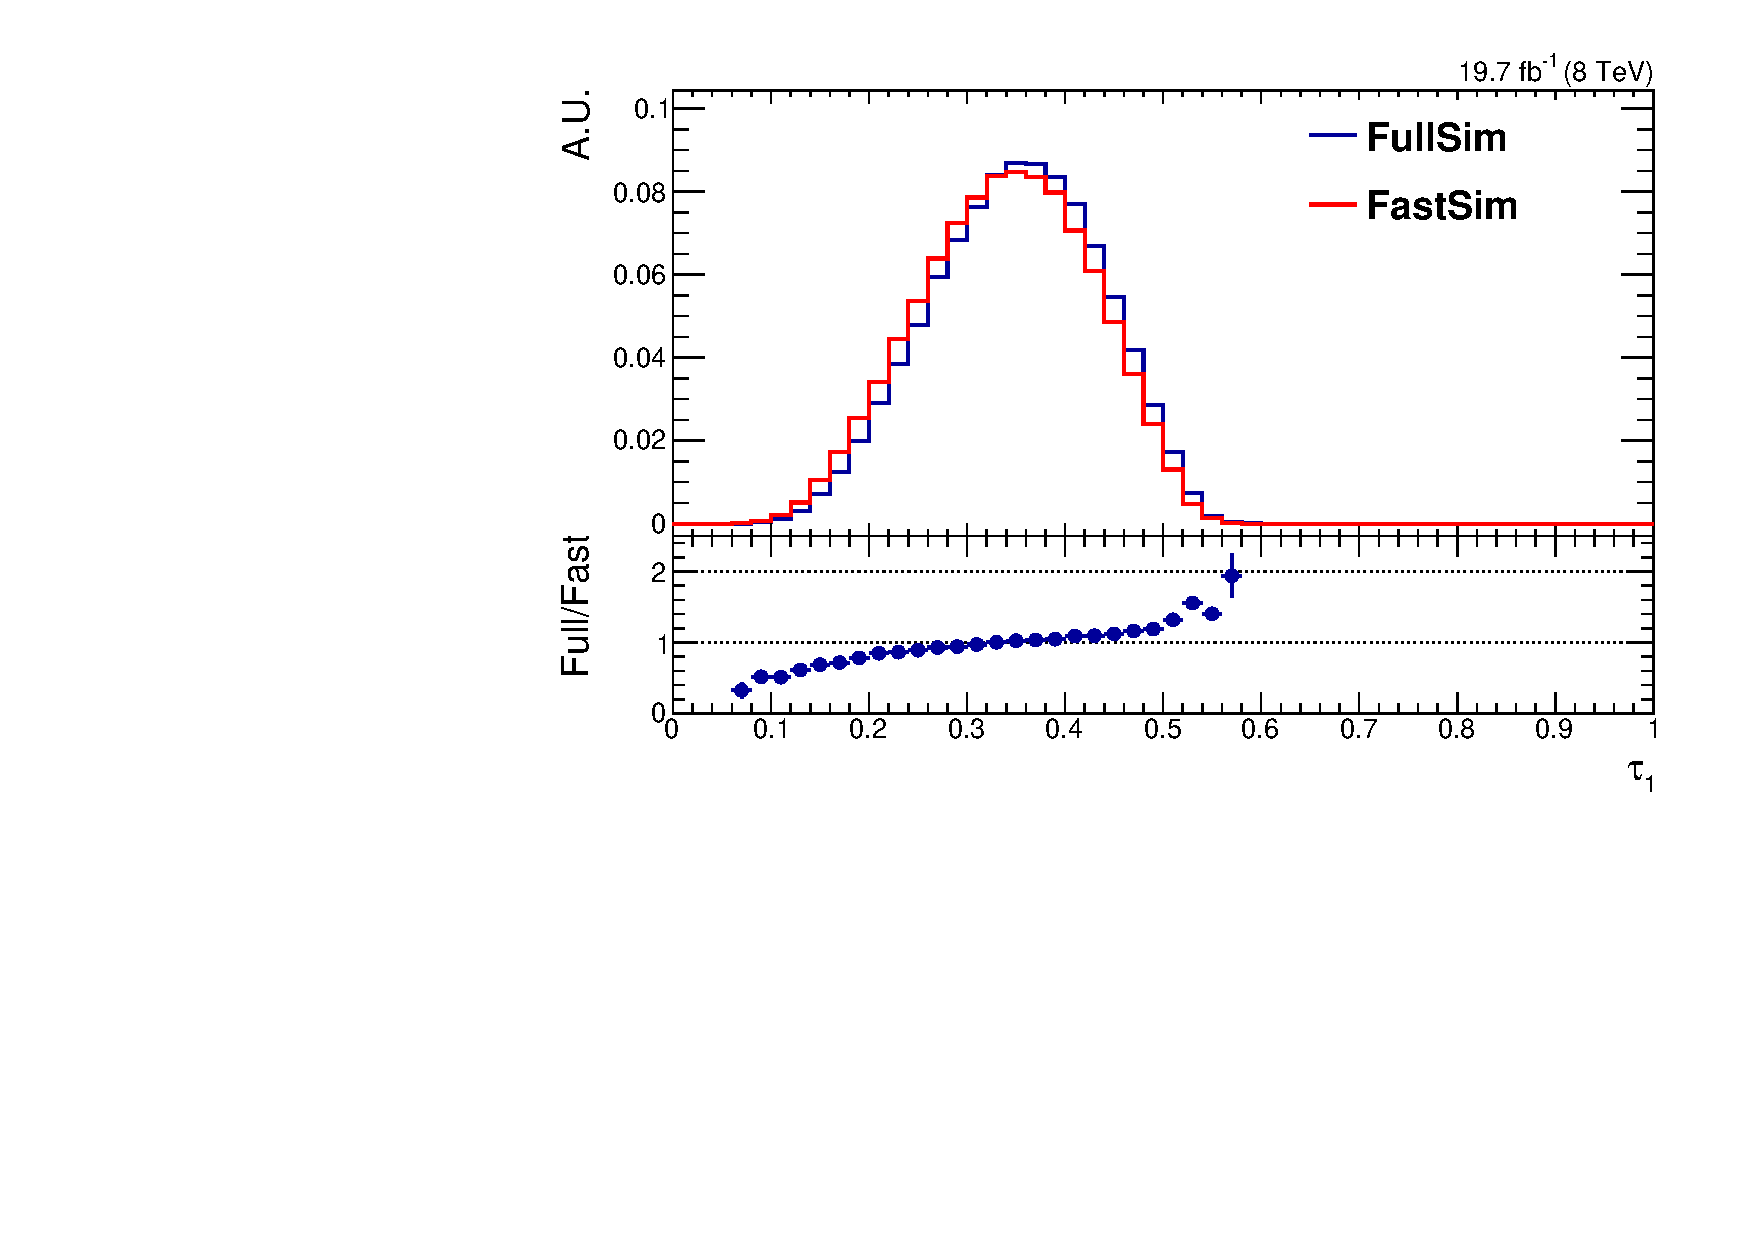
\includegraphics[width=0.49\textwidth]{figures/razor_wtag/FastFull_comparison_TTJets_tau1_masscut}
\caption{Distribution of $\tau_1$ before (left) and after (right) requiring the pruned CA8 jet to
lie within the $\W$ mass window, $70 < m_{\textrm{jet}} < 100$\GeV, for FastSim and
FullSim $t\bar{t}$.
\label{fig:FastFull_tau1}}
\end{figure}

\begin{figure}[htpb]
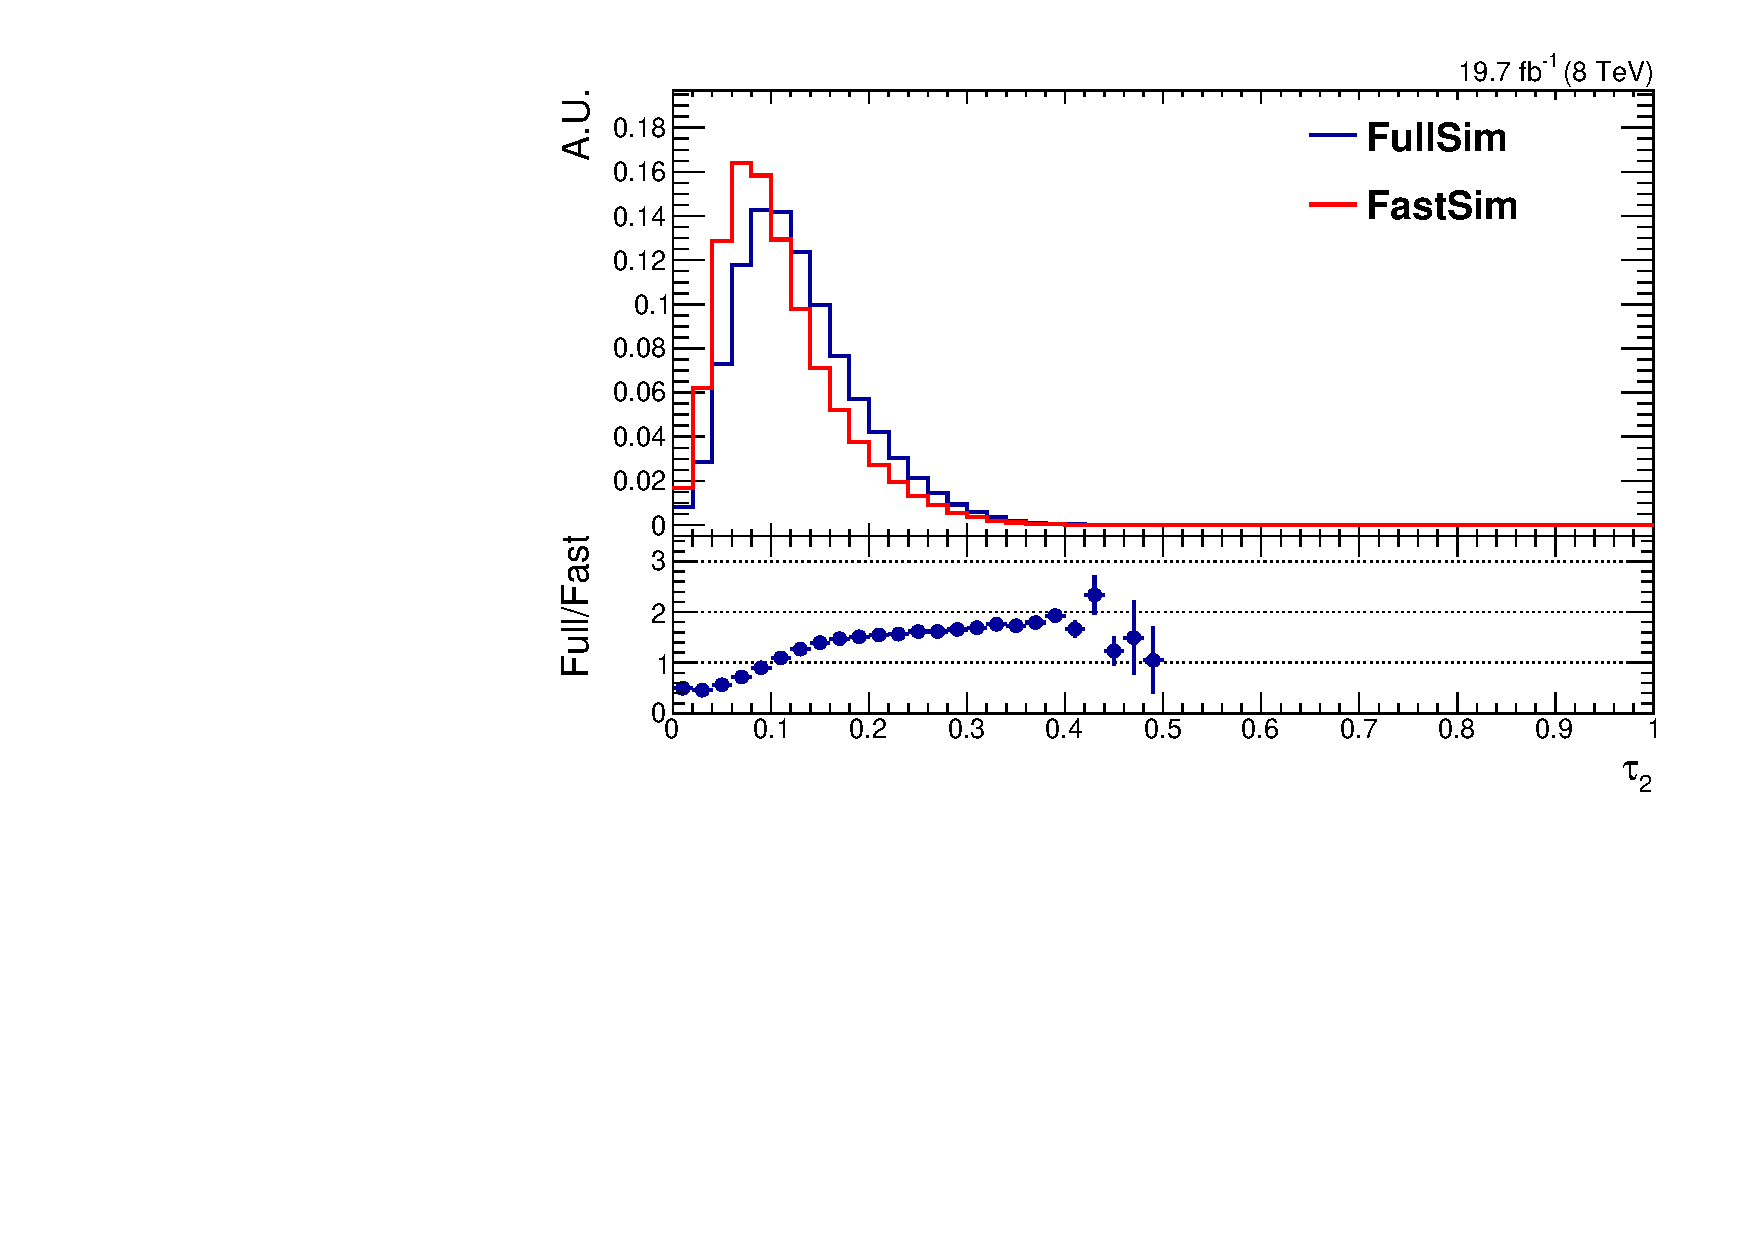
\includegraphics[width=0.49\textwidth]{figures/razor_wtag/FastFull_comparison_TTJets_tau2}
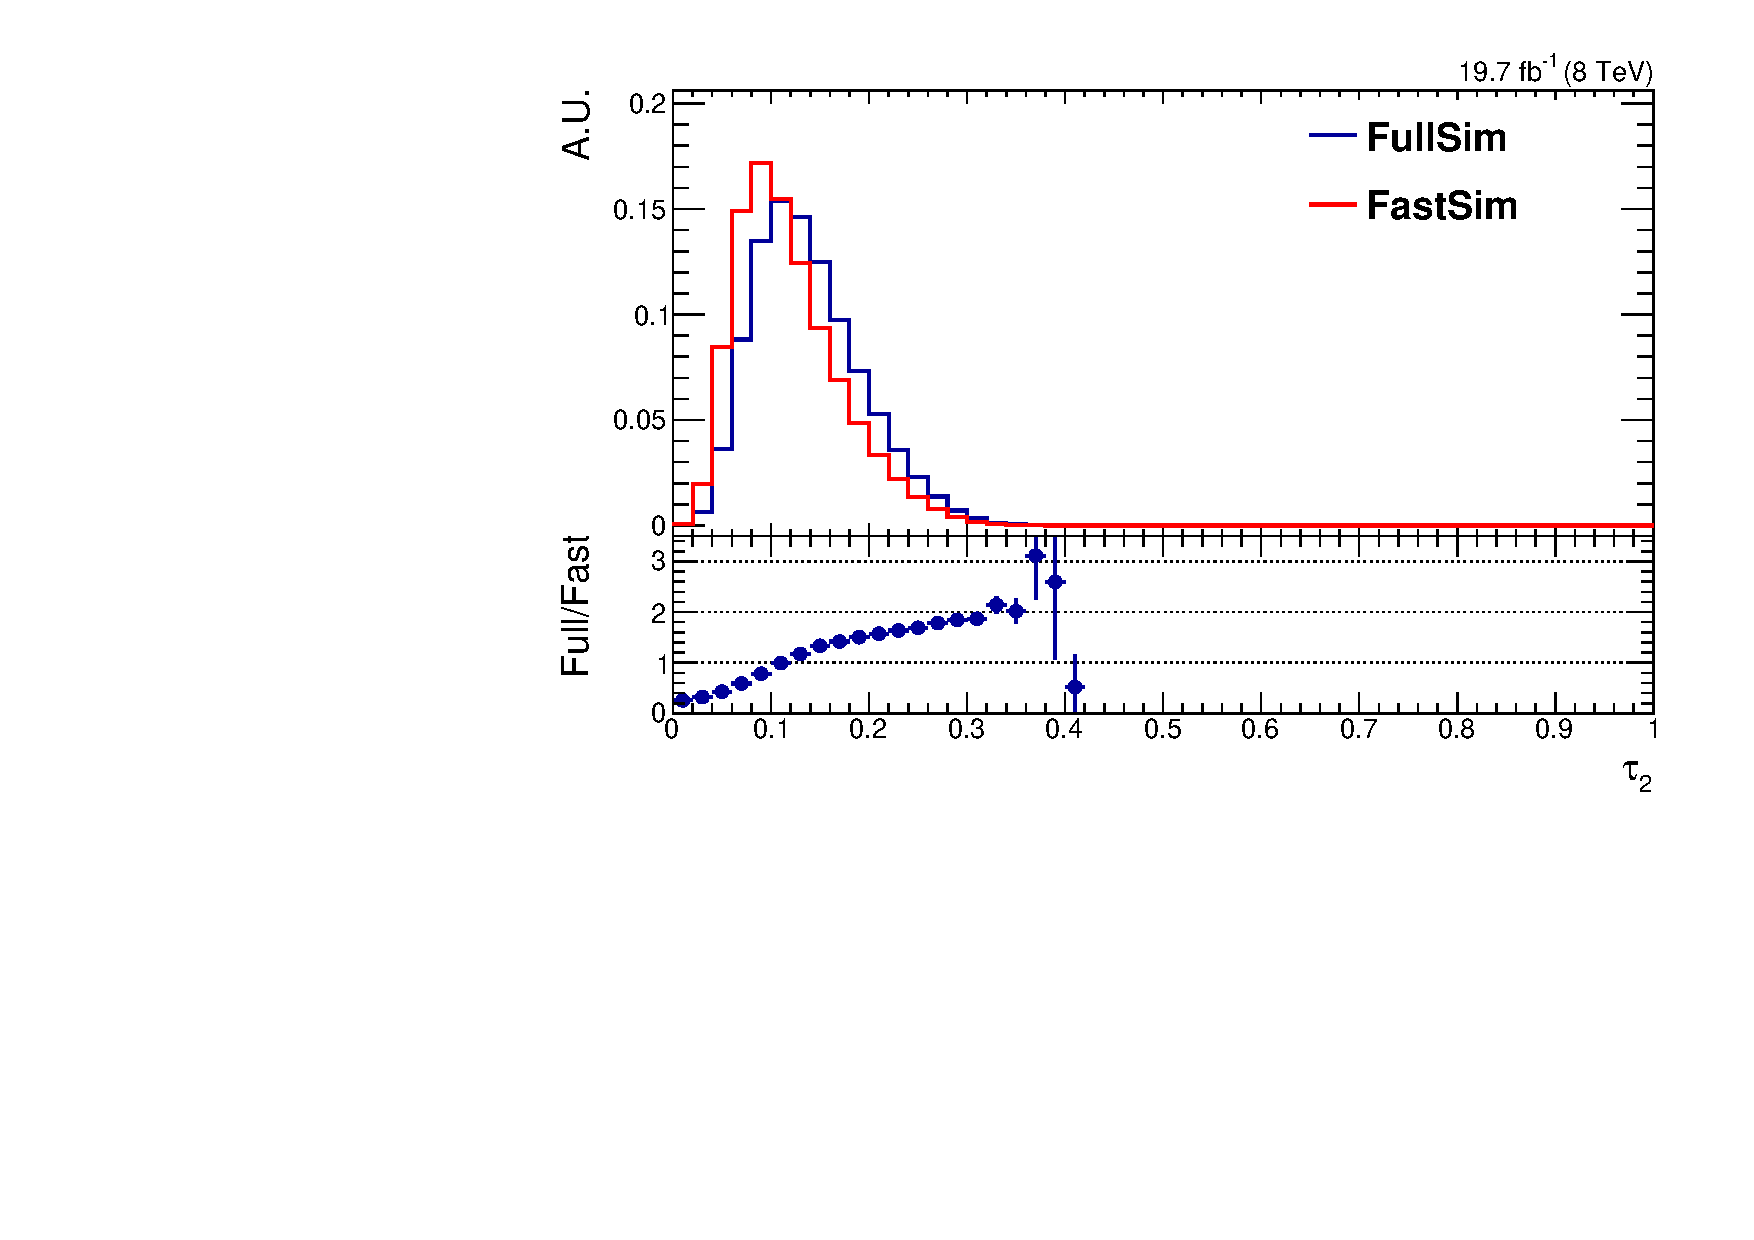
\includegraphics[width=0.49\textwidth]{figures/razor_wtag/FastFull_comparison_TTJets_tau2_masscut}
\caption{Distribution of $\tau_2$ before (left) and after (right) requiring the pruned CA8 jet to
lie within the $\W$ mass window, $70 < m_{\textrm{jet}} < 100$\GeV, for FastSim and FullSim
$t\bar{t}$.
\label{fig:FastFull_tau2}}
\end{figure}

\begin{figure}[htpb]
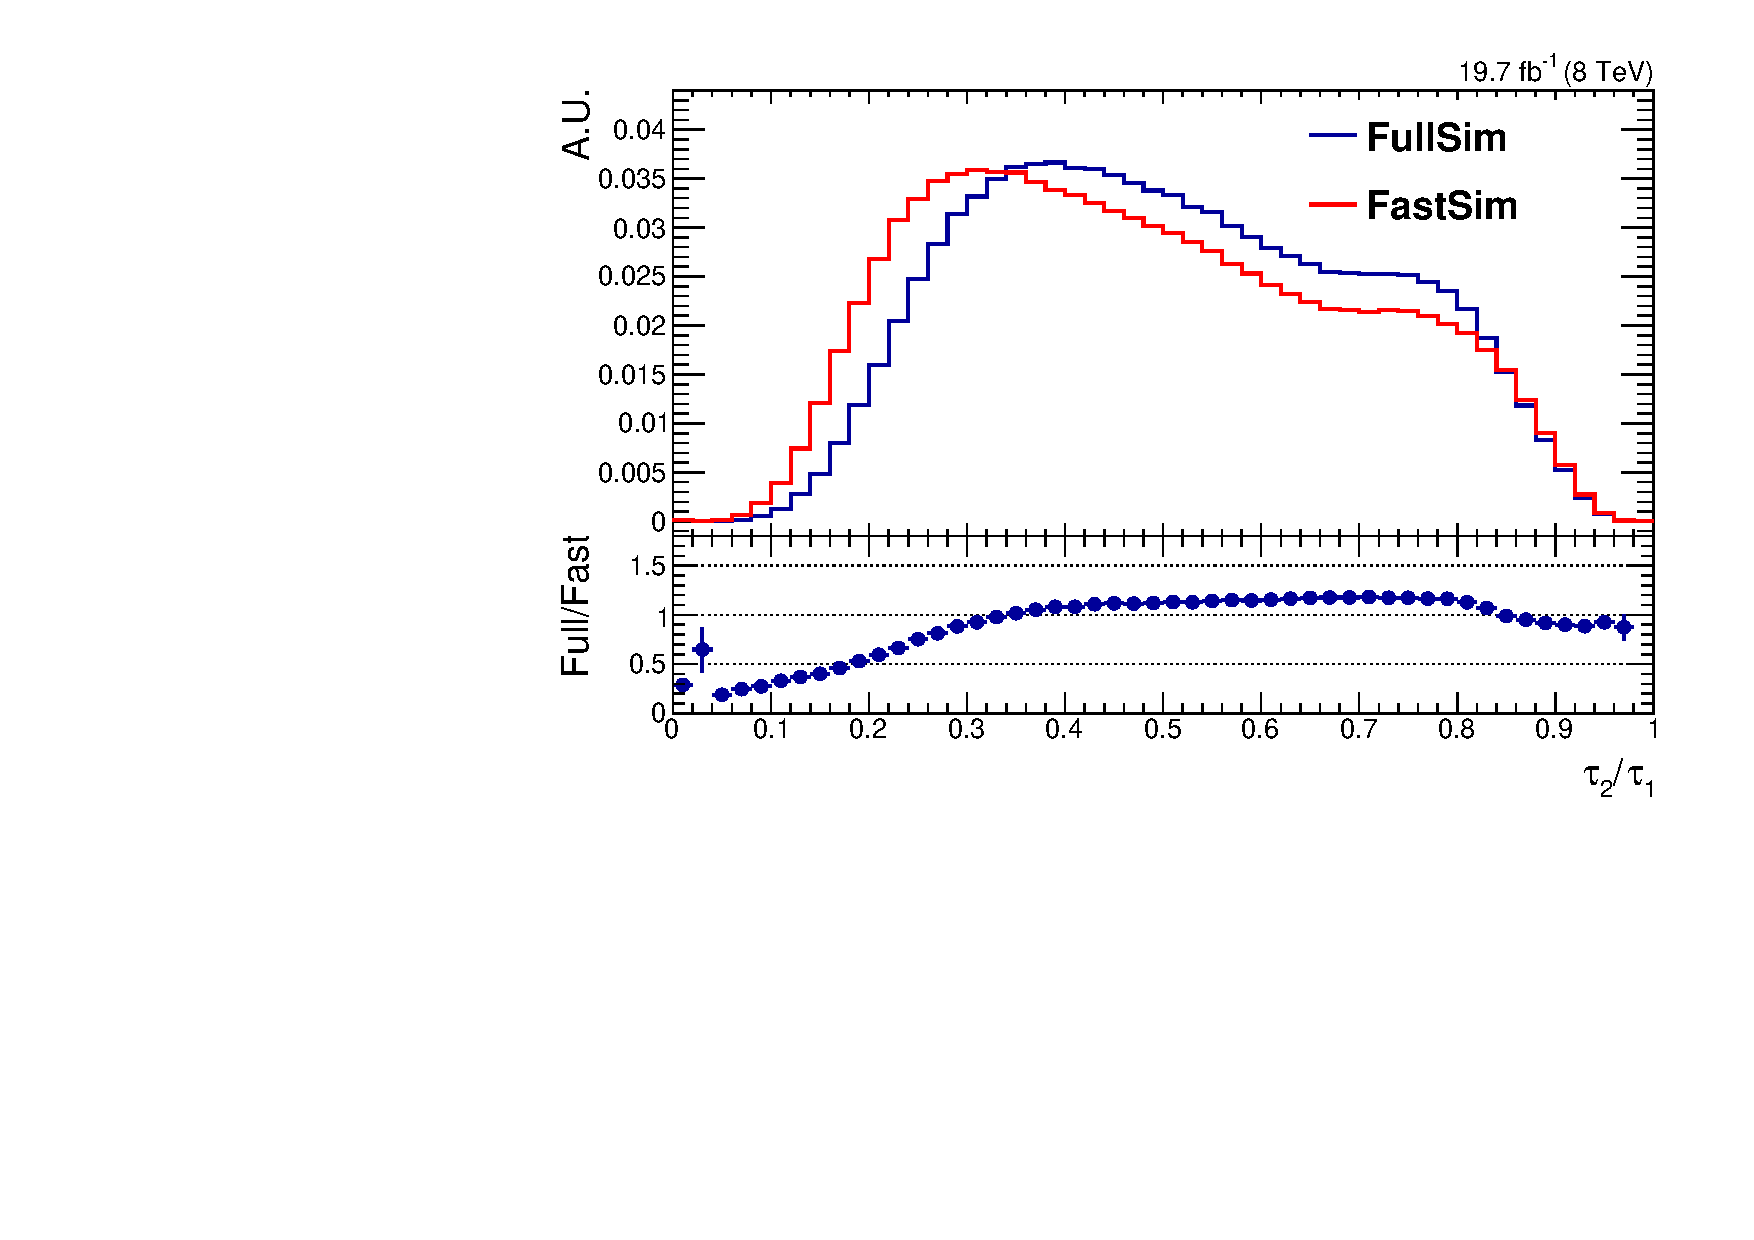
\includegraphics[width=0.49\textwidth]{figures/razor_wtag/FastFull_comparison_TTJets_tau21}
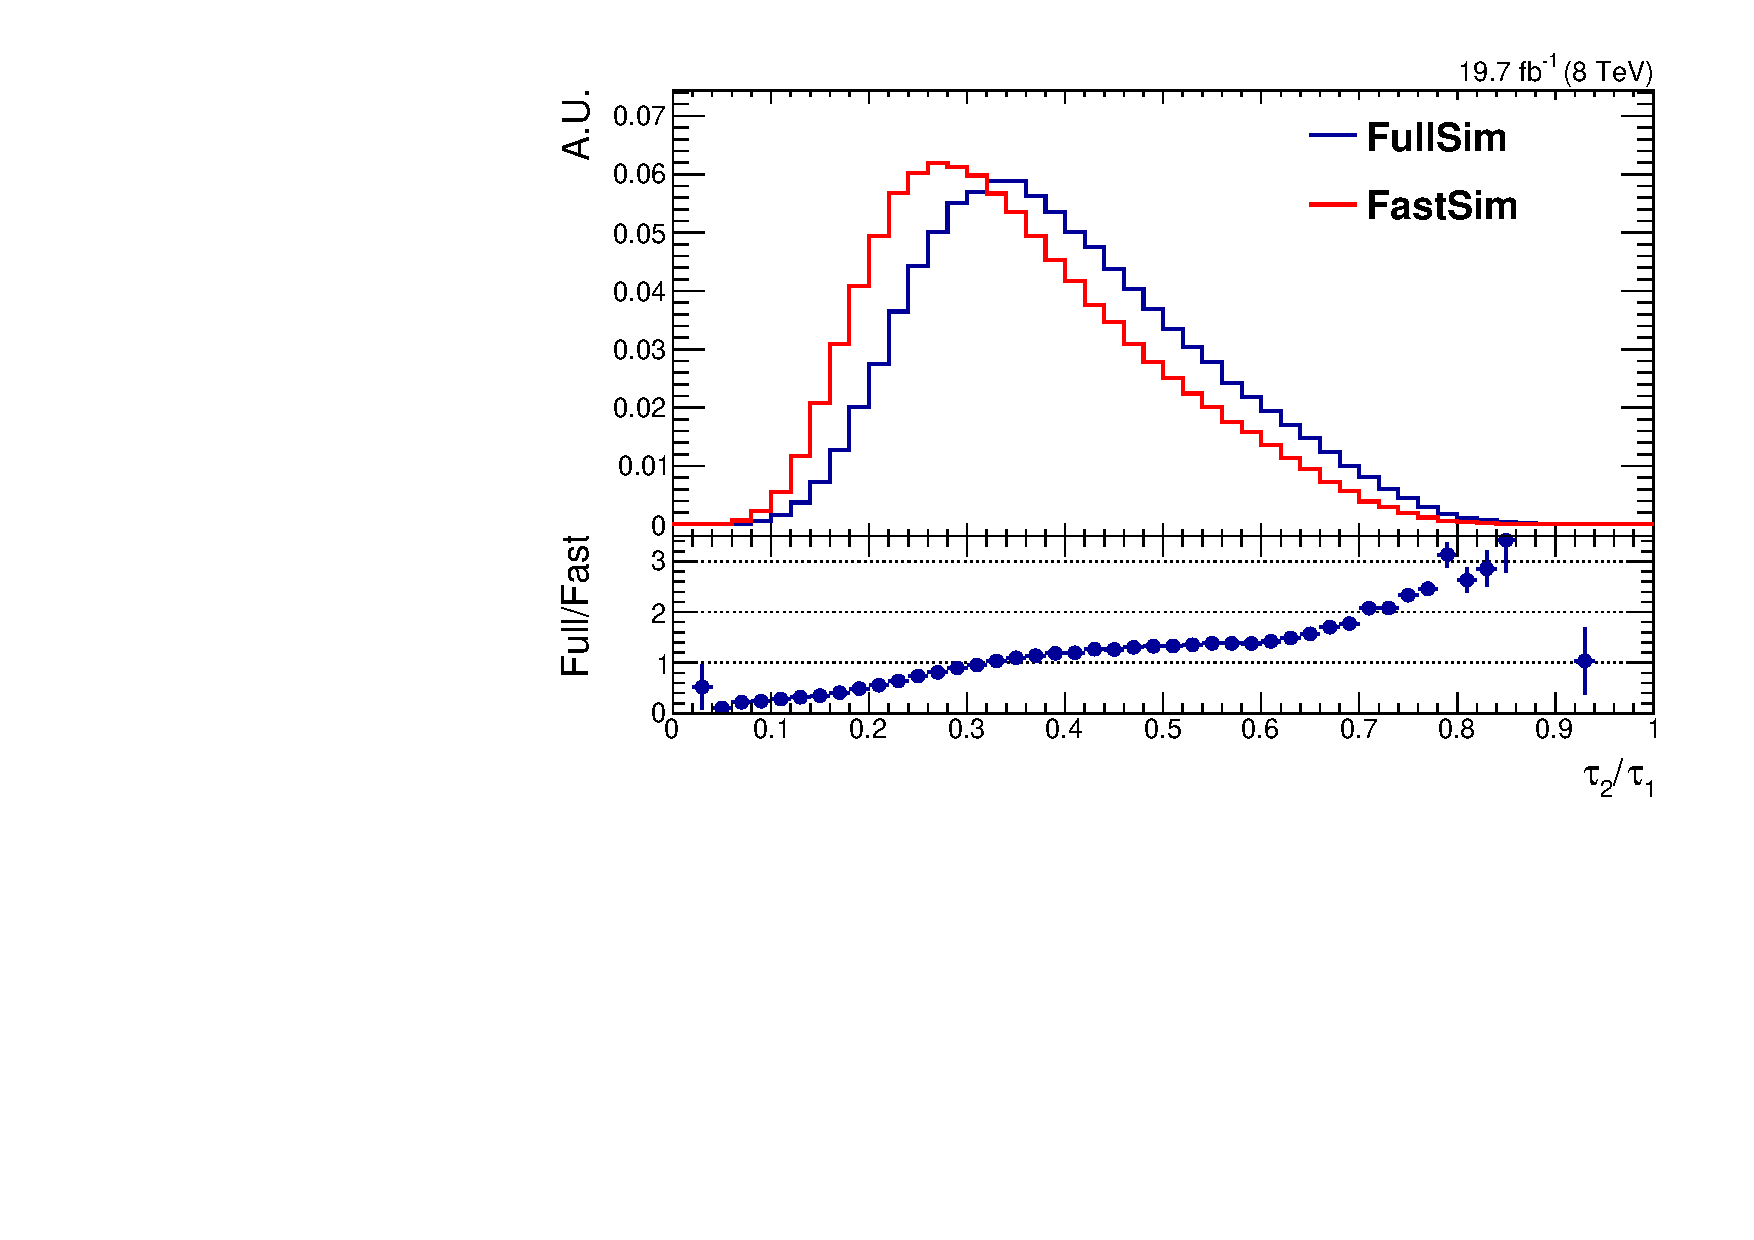
\includegraphics[width=0.49\textwidth]{figures/razor_wtag/FastFull_comparison_TTJets_tau21_masscut}
\caption{Distribution of $\tau_2/\tau_1$ before (left) and after (right) requiring the pruned CA8
jet to lie within the $\W$ mass window, $70 < m_{\textrm{jet}} < 100$\GeV, for FastSim and FullSim
$t\bar{t}$.
\label{fig:FastFull_tau21}}
\end{figure}

These figures also illustrate some of the features of the N-subjettiness variables.
Consider first the $\tau_1$ distribution in Fig.~\ref{fig:FastFull_tau1}. Without a jet mass
requirement, the distibution is quite broad and bimodal. Once the jet mass is required to
be consistent with the $\W$ boson mass, the lower part of the distribution disappears. This
illustrates that quark/gluon jets are expected to have only a single subjet, resulting in a small
$\tau_1$ value. For jets that result from the decay of a $\W$ boson, $\tau_1$ takes on a larger
value. 
This effect is not seen for the $\tau_2$ distributions (Fig.~\ref{fig:FastFull_tau2}), which is
expected because $\tau_2$ quantifies the compatibility with having two or fewer subjets. 
The ratio $\tau_2/\tau_1$, shown on Fig.~\ref{fig:FastFull_tau21}, also displays the
expected behavior: the part of the distribution at high values is removed when requiring the jet
mass to be within the $\W$ mass window, and thus when selecting more jets with two-prong decays. 

The procedure to determine the $\W$ boson tagging efficiency for both Fastsim and FullSim is the
following:
\begin{enumerate}
\item Filter the events at the generator level, requiring the presence of exactly one hadronically
decaying $\W$ boson. 
\item For the generated $\W$ boson, find the closest reconstructed CA8 jet, and require that it be
within $\Delta R = 0.8$ from the $\W$ boson. If no such jet exists, the event is discarded.  
\item Require that there be no (generator-level) $\cPqb$ quark from the top quark decay within the
cone of the selected CA8 jet. (We wish to select boosted $\W$ bosons only, not boosted top quarks.)
\item For the events that pass the above selection, consider the $\pt$ distribution of the CA8 jet
at two selection levels:
 \begin{itemize}
   \item no additional selection
   \item $70 < m_\textrm{jet} < 100$\GeV and $\tau_2/\tau_1 < 0.5$
 \end{itemize}
\item By dividing those \pt distributions we obtain the $\W$ boson tagging efficiency. 
\end{enumerate}
To derive the FullSim/FastSim scale factor for the $\W$ boson tagging efficiency, we divide the
efficiencies $\epsilon$ obtained in FullSim and FastSim:
\begin{equation}
SF_{\textrm{Full/Fast}}(\pt) =
\frac{\epsilon_{\textrm{FullSim}}(\pt)}{\epsilon_{\textrm{FastSim}}(\pt)}.
\end{equation}
A graphical representation of the $\W$ boson tag efficiency in FastSim and FullSim is shown on
Fig.~\ref{fig:boost_Wfullfast} for a fine and more coarse binning in CA8 jet \pt. The resulting
scale factor is shown for the final, coarse binning that will be used to rescale the signal
simulation. 
Table~\ref{tab:SF_FullFast} summarizes the $\W$ boson tag efficiency FullSim/FastSim scale factor
with its
statistical uncertainty.

\begin{figure}[htbp]
\centering
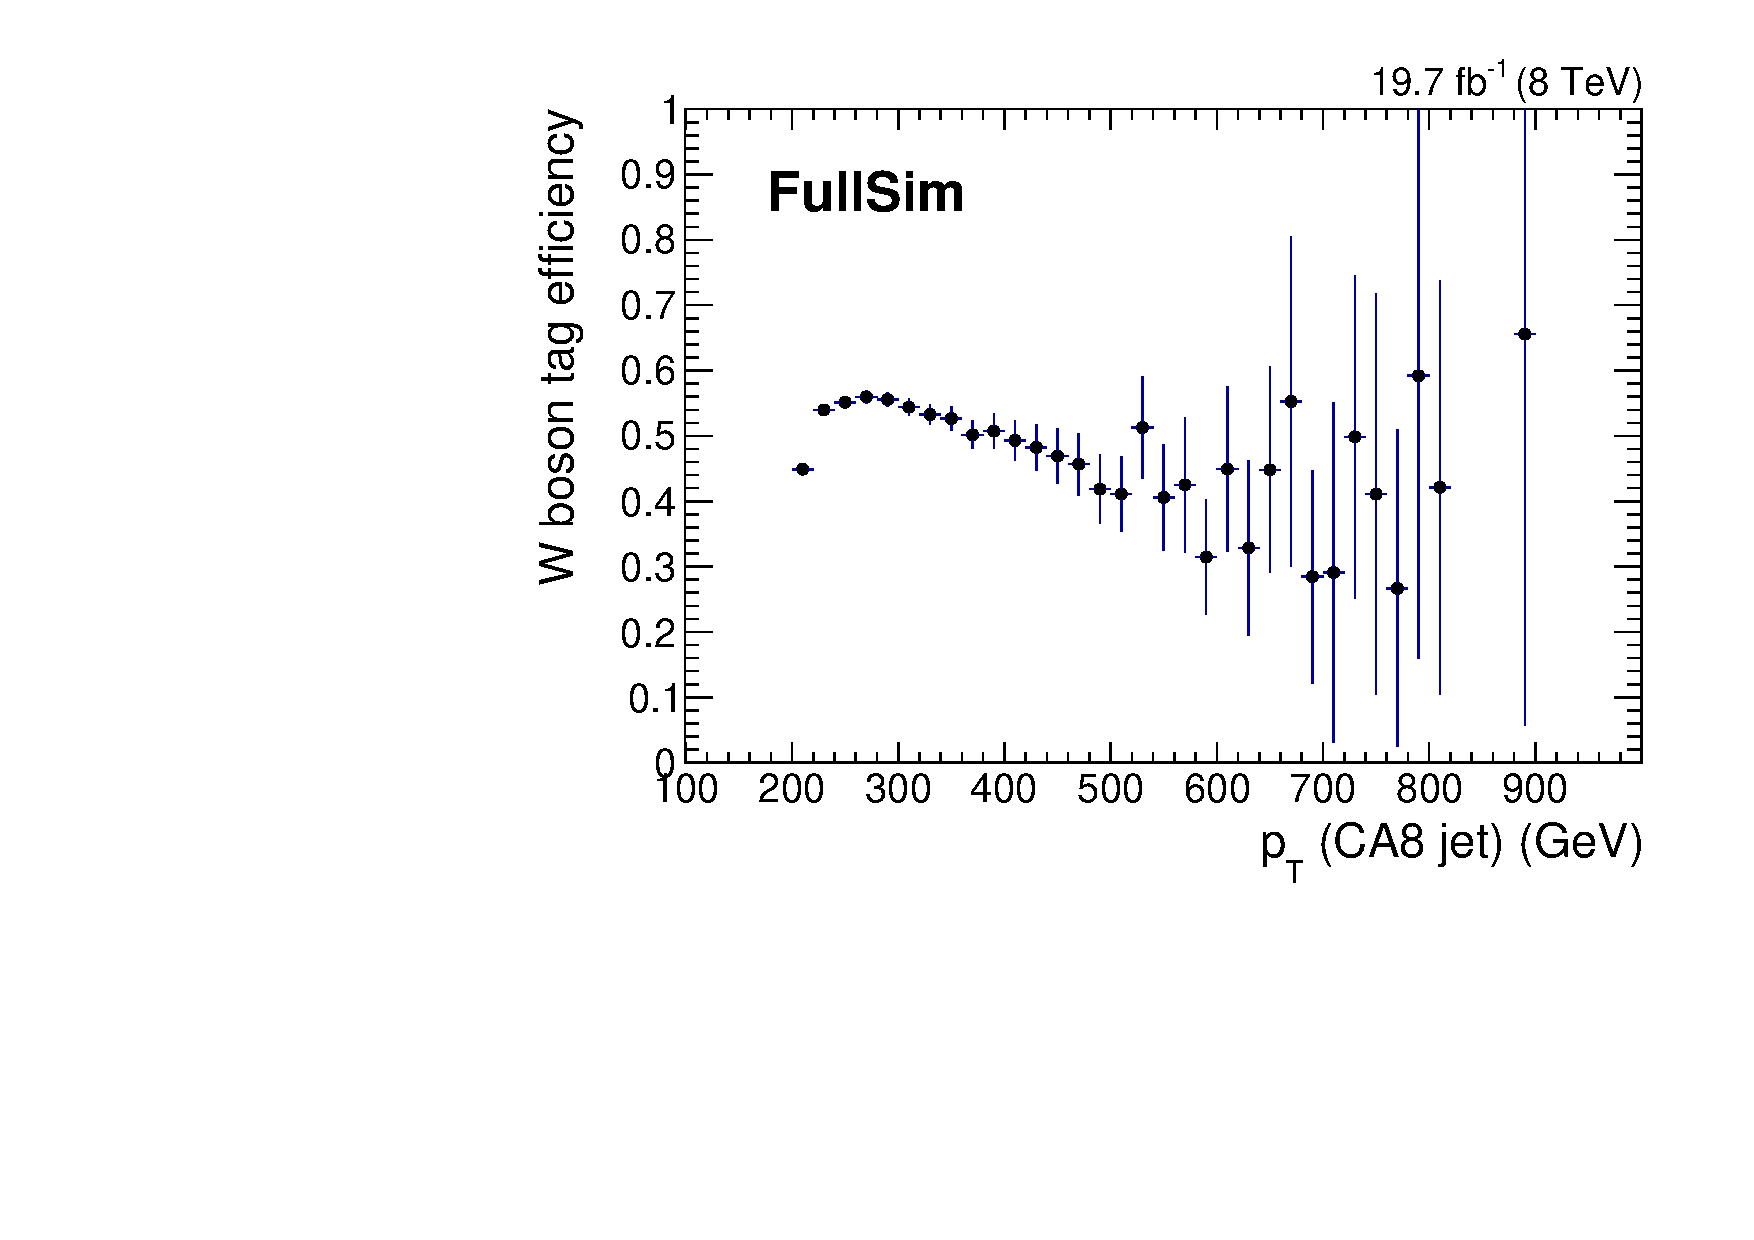
\includegraphics[width=0.48\textwidth]{figures/razor_wtag/Eff_ratio_tagged_all_FullSim_Thesis}
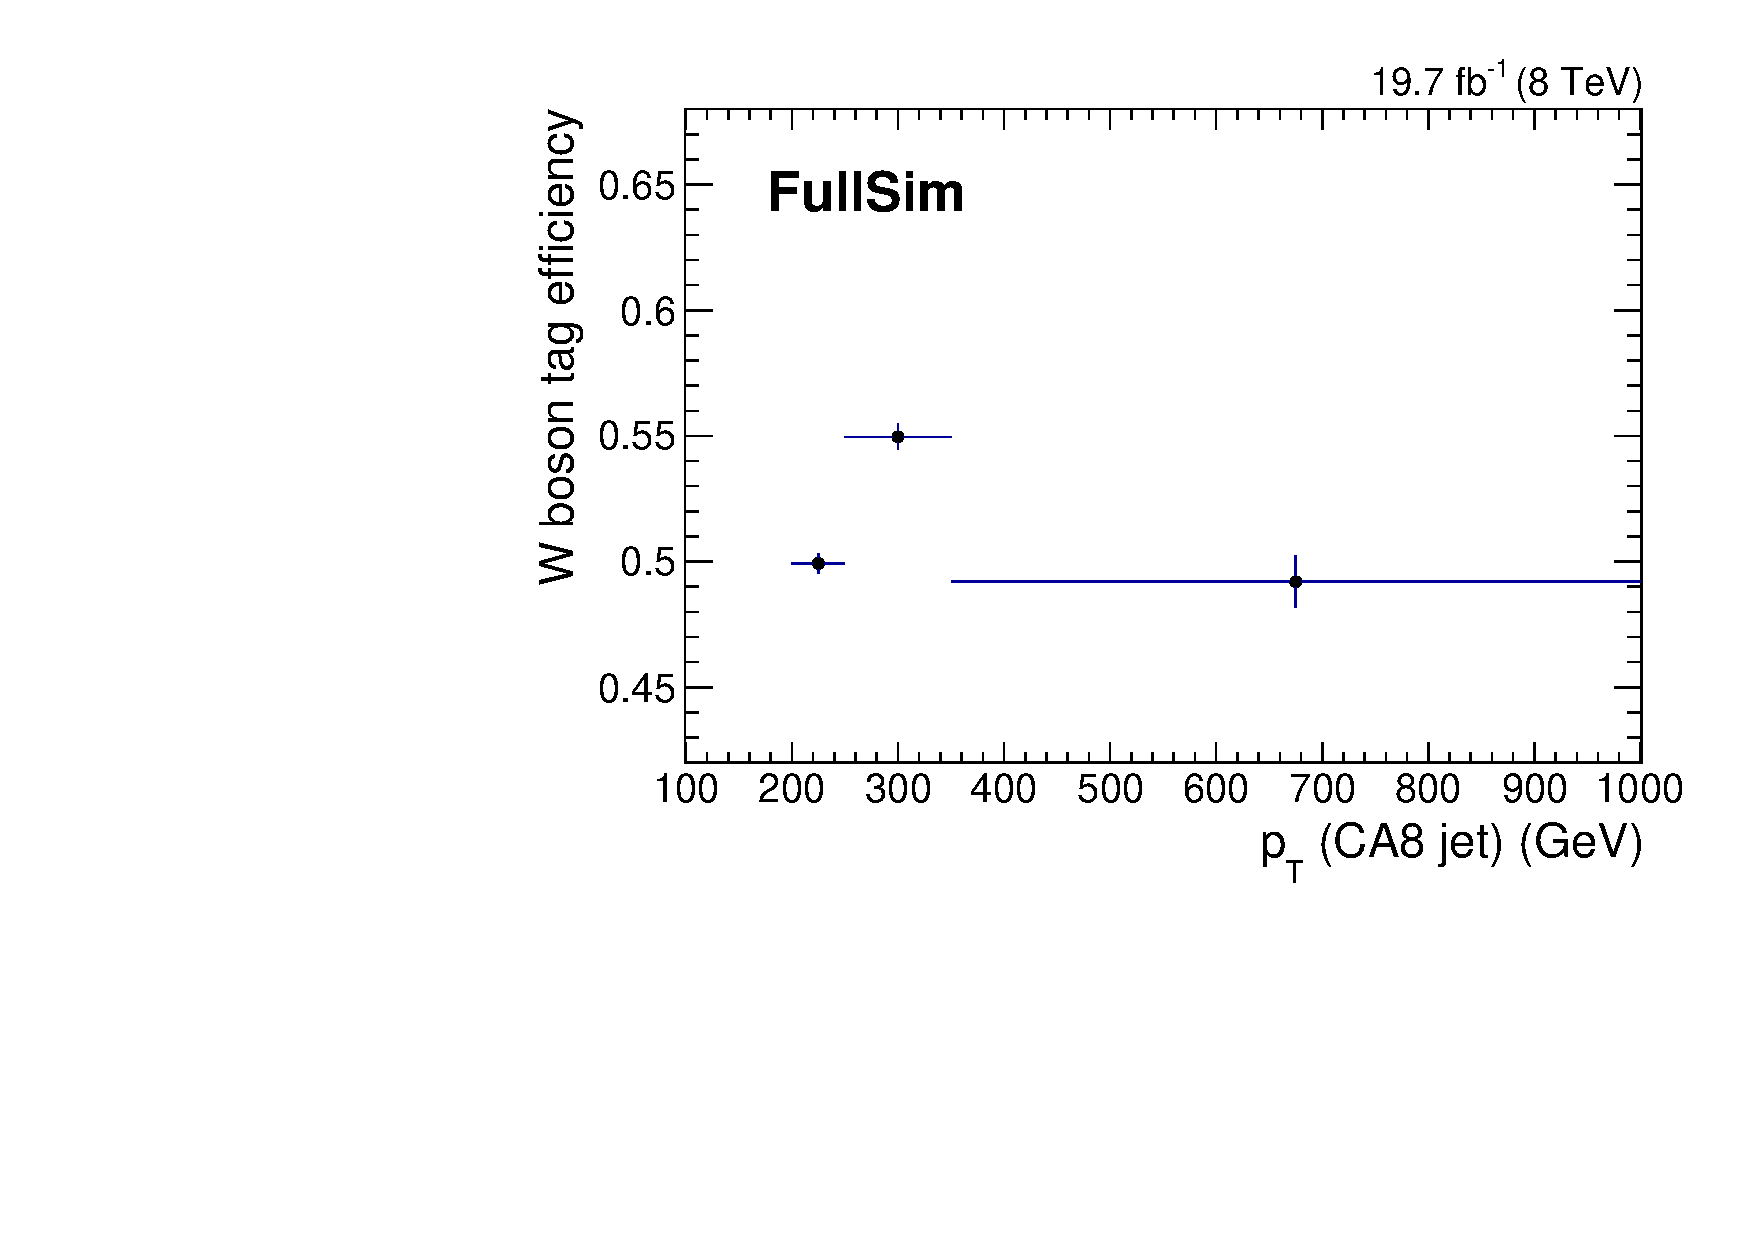
\includegraphics[width=0.48\textwidth]
{figures/razor_wtag/Eff_ratio_tagged_all_varbin_FullSim_Thesis}

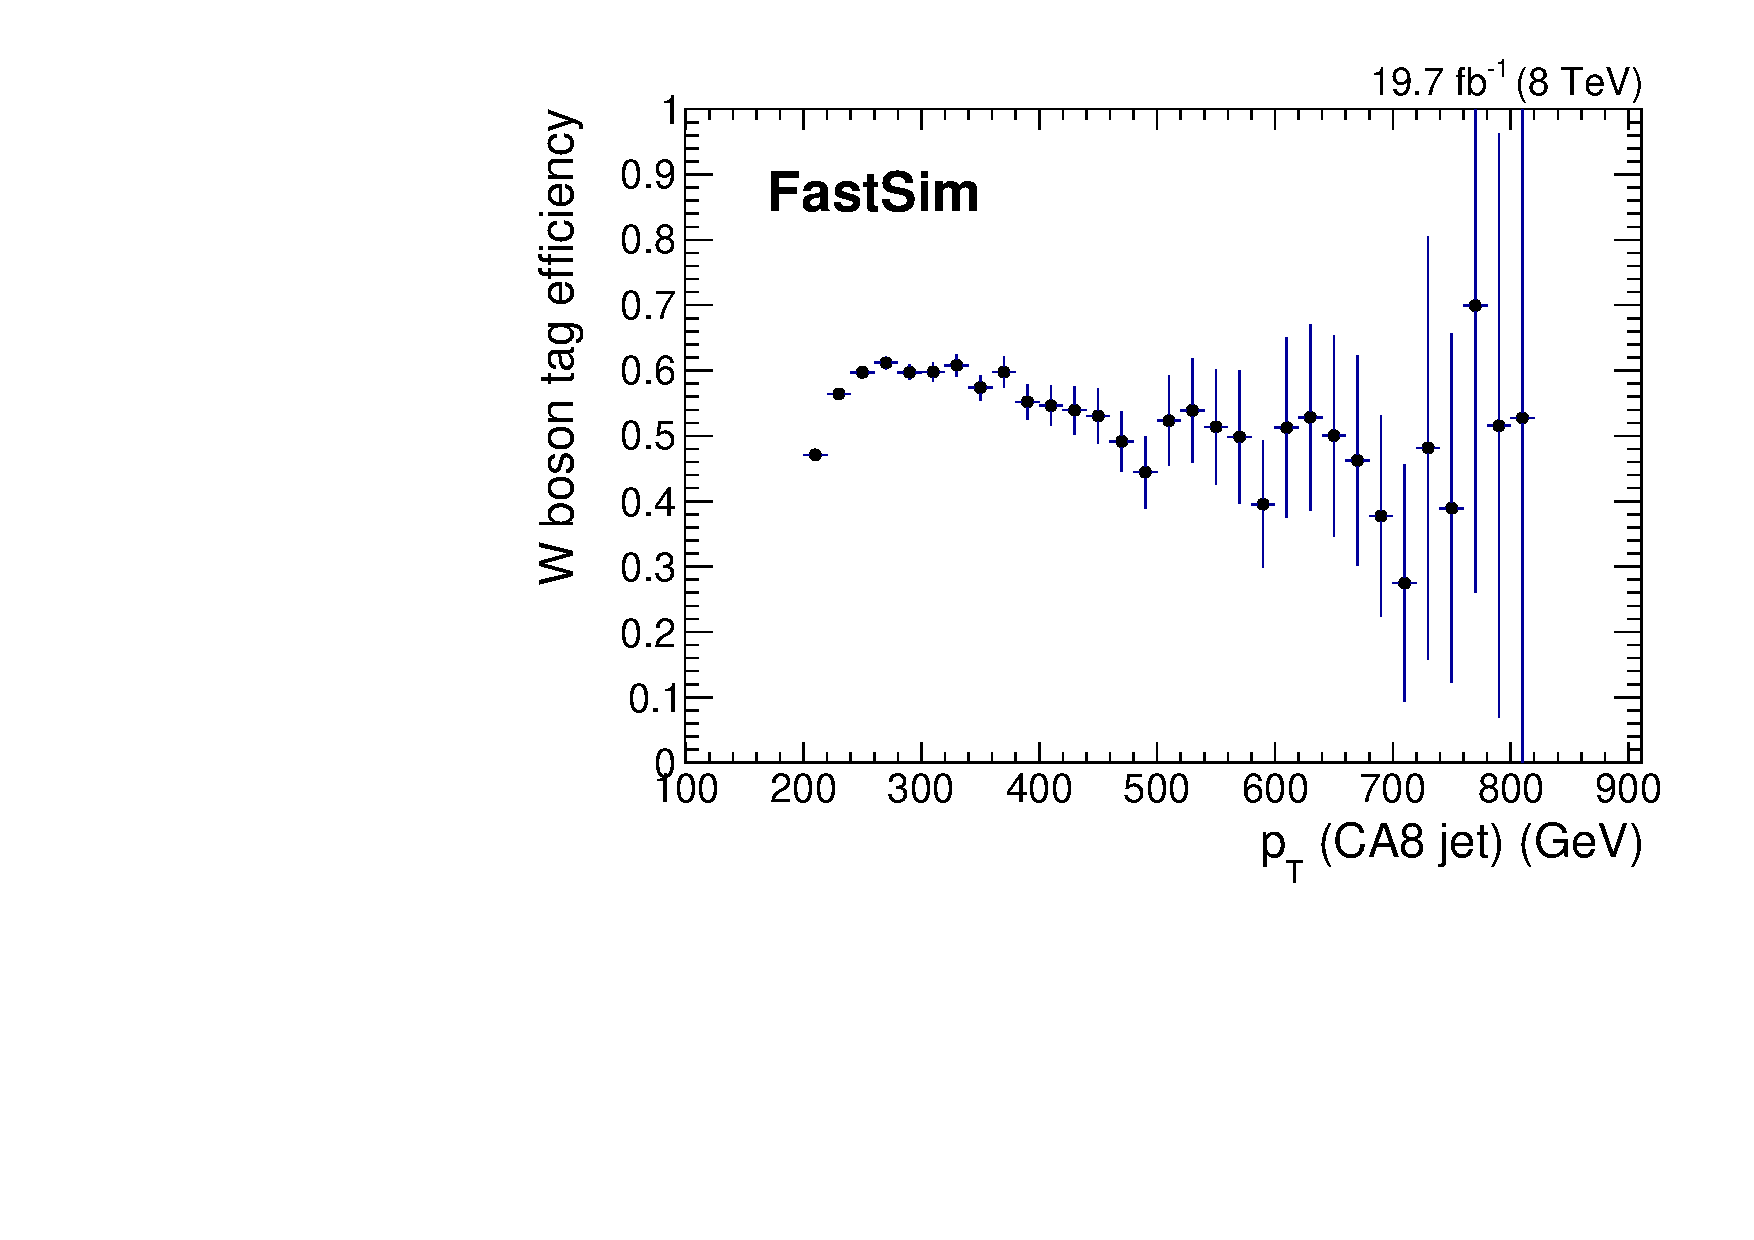
\includegraphics[width=0.48\textwidth]{figures/razor_wtag/Eff_ratio_tagged_all_FastSim_Thesis}
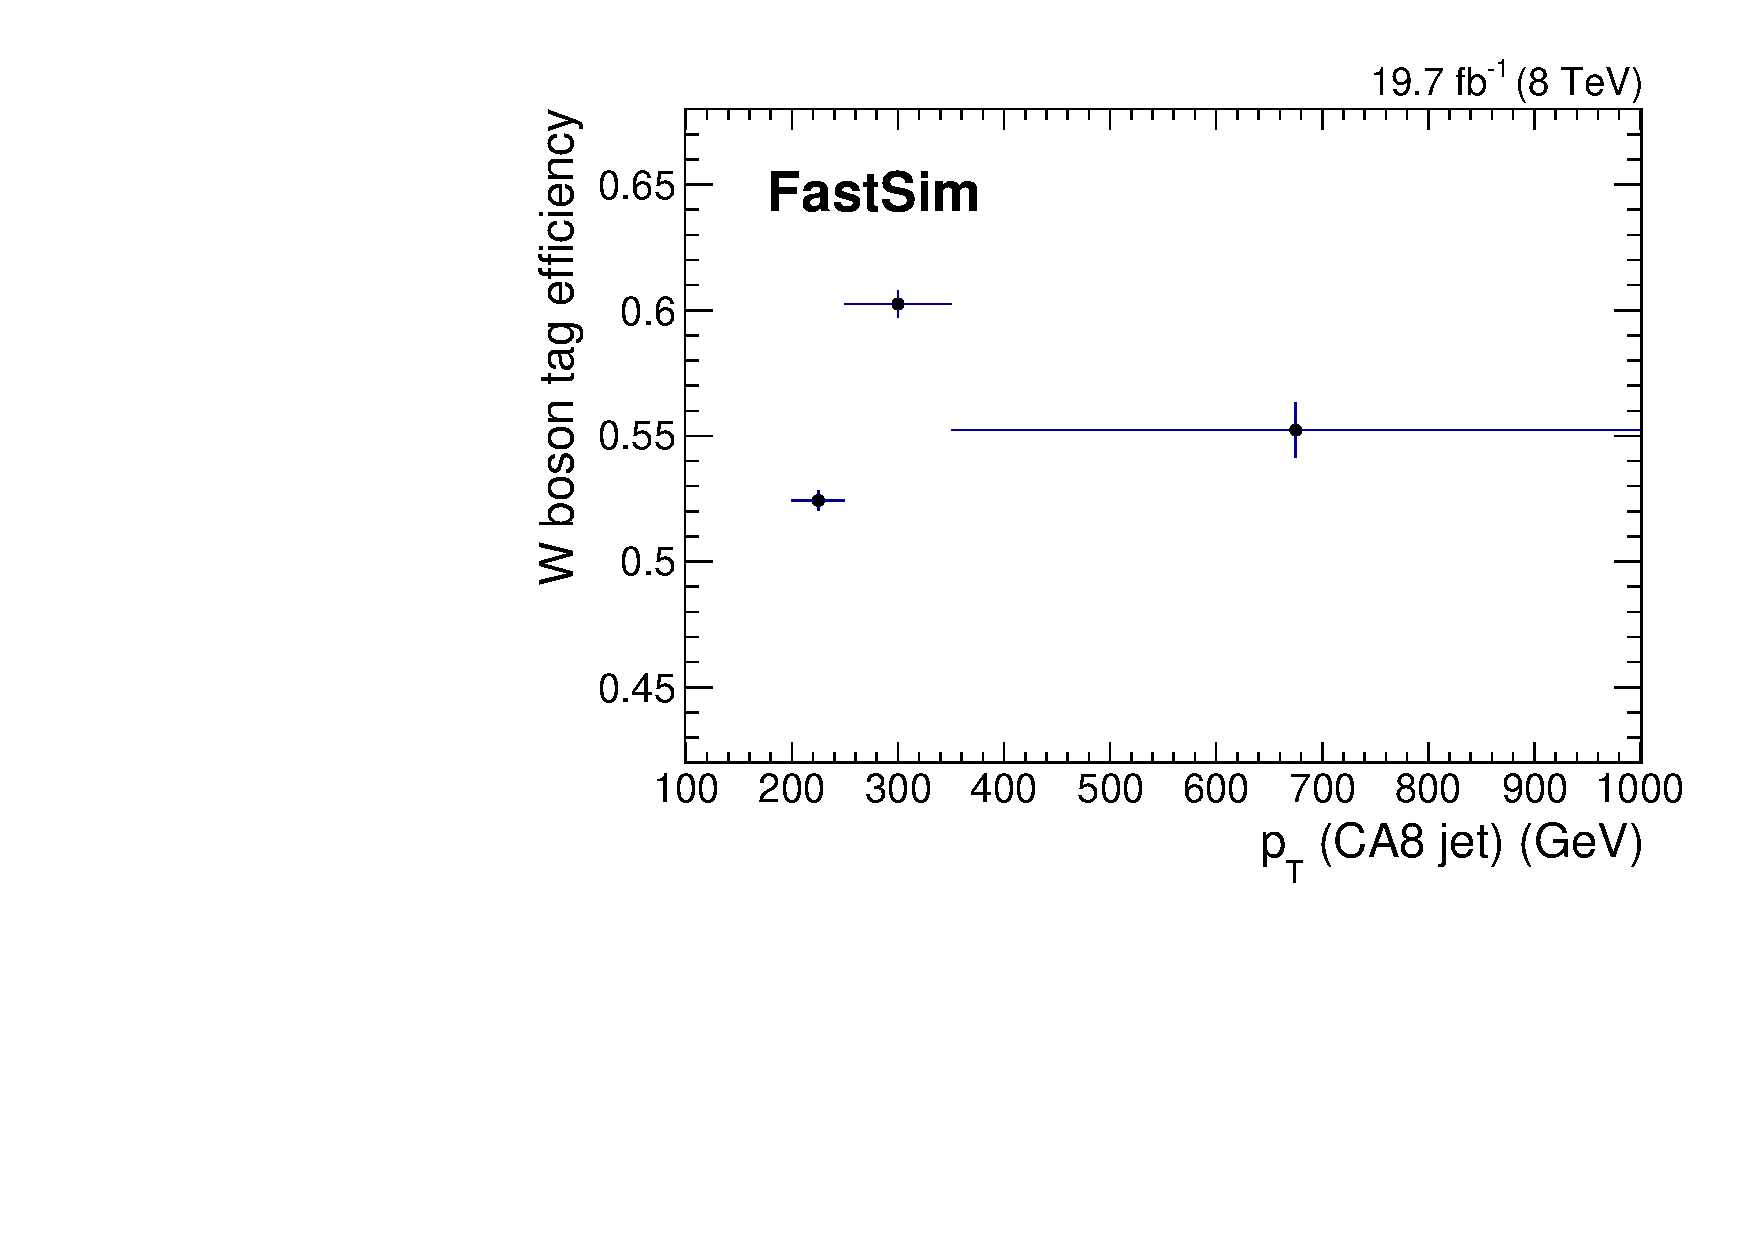
\includegraphics[width=0.48\textwidth]
{figures/razor_wtag/Eff_ratio_tagged_all_varbin_FastSim_Thesis}

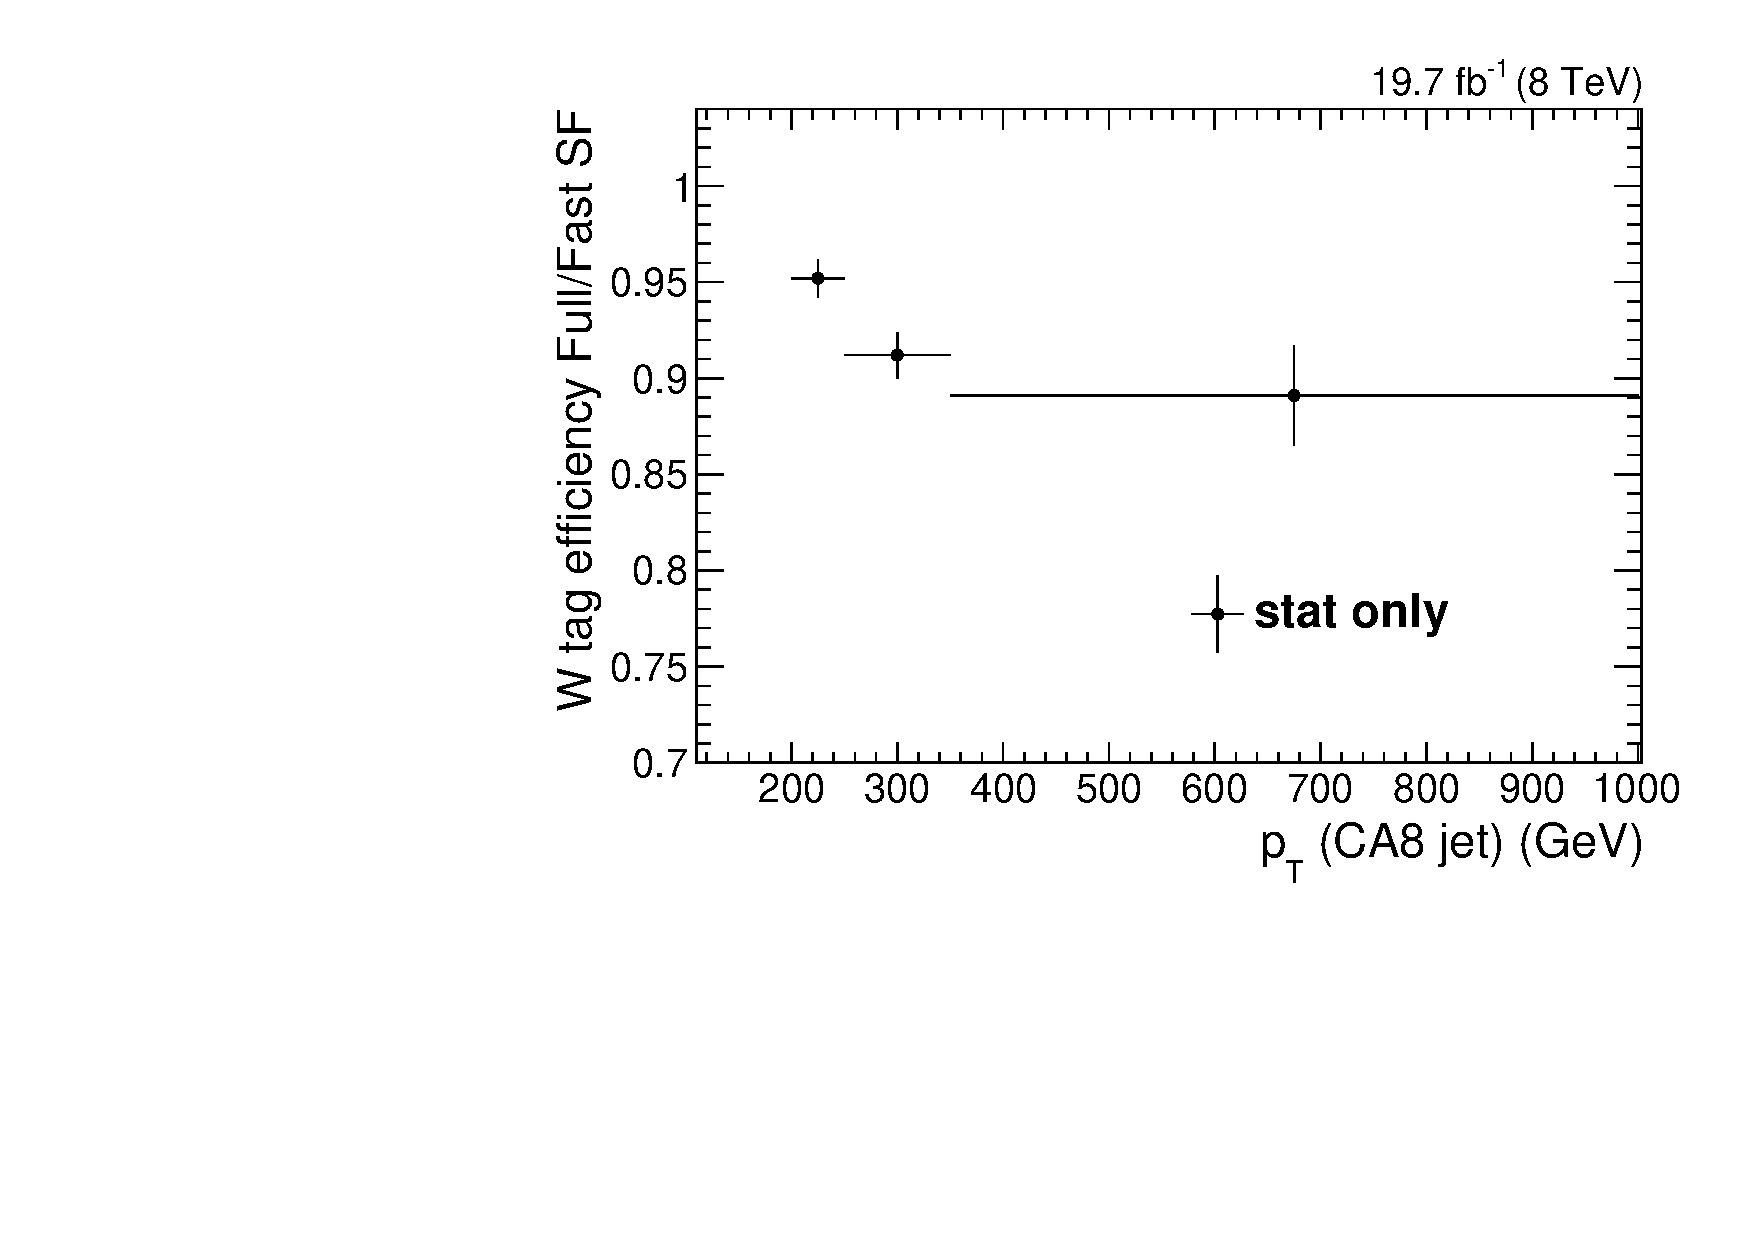
\includegraphics[width=0.6\textwidth]{figures/razor_wtag/SF_FullFast_Thesis}
\caption{[top] $\W$ boson tag efficiency versus CA8 jet \pt, with two different binnings, obtained
from FullSim $t\bar{t}$ events as described in the text. The shown uncertainties are statistical
only. 
[middle] $\W$ boson tag efficiency versus CA8 jet \pt, with two different binnings, obtained from
FastSim $t\bar{t}$ events as described in the text. The shown uncertainties are statistical only. 
[bottom] $\W$ boson tag FullSim/FastSim efficiency scale factor versus CA8 jet \pt. The shown
uncertainties are statistical only.
\label{fig:boost_Wfullfast}}
\end{figure}

\begin{table}[htpb]
\centering
\caption{Summary of FullSim/FastSim scale factor for the $\W$ tag efficiency}
\vspace{1ex}
\begin{tabular}{c c}
\toprule
CA8 jet $\pt$ (\GeV) & $SF_{\textrm{Full/Fast}}$\\
\midrule
$[200 - 250[$ &  $0.952 \pm 0.010$ \\
$[250 - 350[$ &  $0.912 \pm 0.012$ \\
$[350 - ...]$ &  $0.891 \pm 0.026$ \\
\bottomrule
\end{tabular}
\label{tab:SF_FullFast}
\end{table}


%% ---------------------------------------------------------------------------------------------

\subsubsection{\texorpdfstring{$\W$}{W} boson tag fake rate scale factor \label{sec:wtag_fake_sf}}

The $\W$ boson tag fake rate scale factor is meant to correct processes that do not have
hadronically decaying $\W$ bosons in their final state. As the fake rate depends on the composition
of the sample, this scale factor has to be derived for each analysis separately. 
We will thus need to obtain a sample of events containing misidentified $\W$ boson jets to derive a
dedicated scale factor for the razor boost analysis. A multijet-enriched control region is defined,
using the following selection:
\begin{itemize}
\item no loose leptons, 
\item no $\cPqb$ tagged (CSVL) jets,
\item at least 3 AK5 jets,
\item at least one AK5 jet with $\pt>200$\GeV,
\item small minimum azimuthal angle between the \VEtmiss and the leading three jets, \\
$\Delta\phi_{min} < 0.3$.
\end{itemize}
This selection is similar to the baseline selection employed in the rest of the analysis. The
kinematic regime, and the composition of the sample will thus also be similar. The main difference
is that we have not applied any selection on \mr or \rsq, in order to retain a higher statistical
power. 

To obtain the fake rates $\epsilon$ for $\W$ boson tagging we use the leading CA8 jet in each
event, and check whether it is tagged by the $\W$ boson tagger. After obtaining the
fake rates in both data and simulation, we compute the scale factor as their ratio,
\begin{equation}
SF_\textrm{Wtag}^\textrm{fake}(\pt) =
\frac{\epsilon^{\textrm{data}}(\pt)}{\epsilon^{\textrm{simulation}}(\pt)}.
\end{equation} 
In the calculation of the uncertainties on this scale factor we include the statistical uncertainty,
as well as the trigger efficiency and jet energy scale uncertainties for both AK5 and CA8 jets. 
All three uncertainties are varied up (down) at the same time to get the overall up (down)
systematic  uncertainty.
The fake rate in data and simulation, as well as the resulting $\W$ boson tag fake rate scale factor
are shown in Fig.~\ref{fig:boost_wfake}. As we can see from the figure, there is a drop in the scale
factor just above a \pt of 300\GeV. This is a result of a residual mismodelling of the trigger
efficiency. 

%\textcolor{red}{TODO: add more information on this "wiggle", perhaps in an appendix.}

\begin{figure}[htbp]
\centering
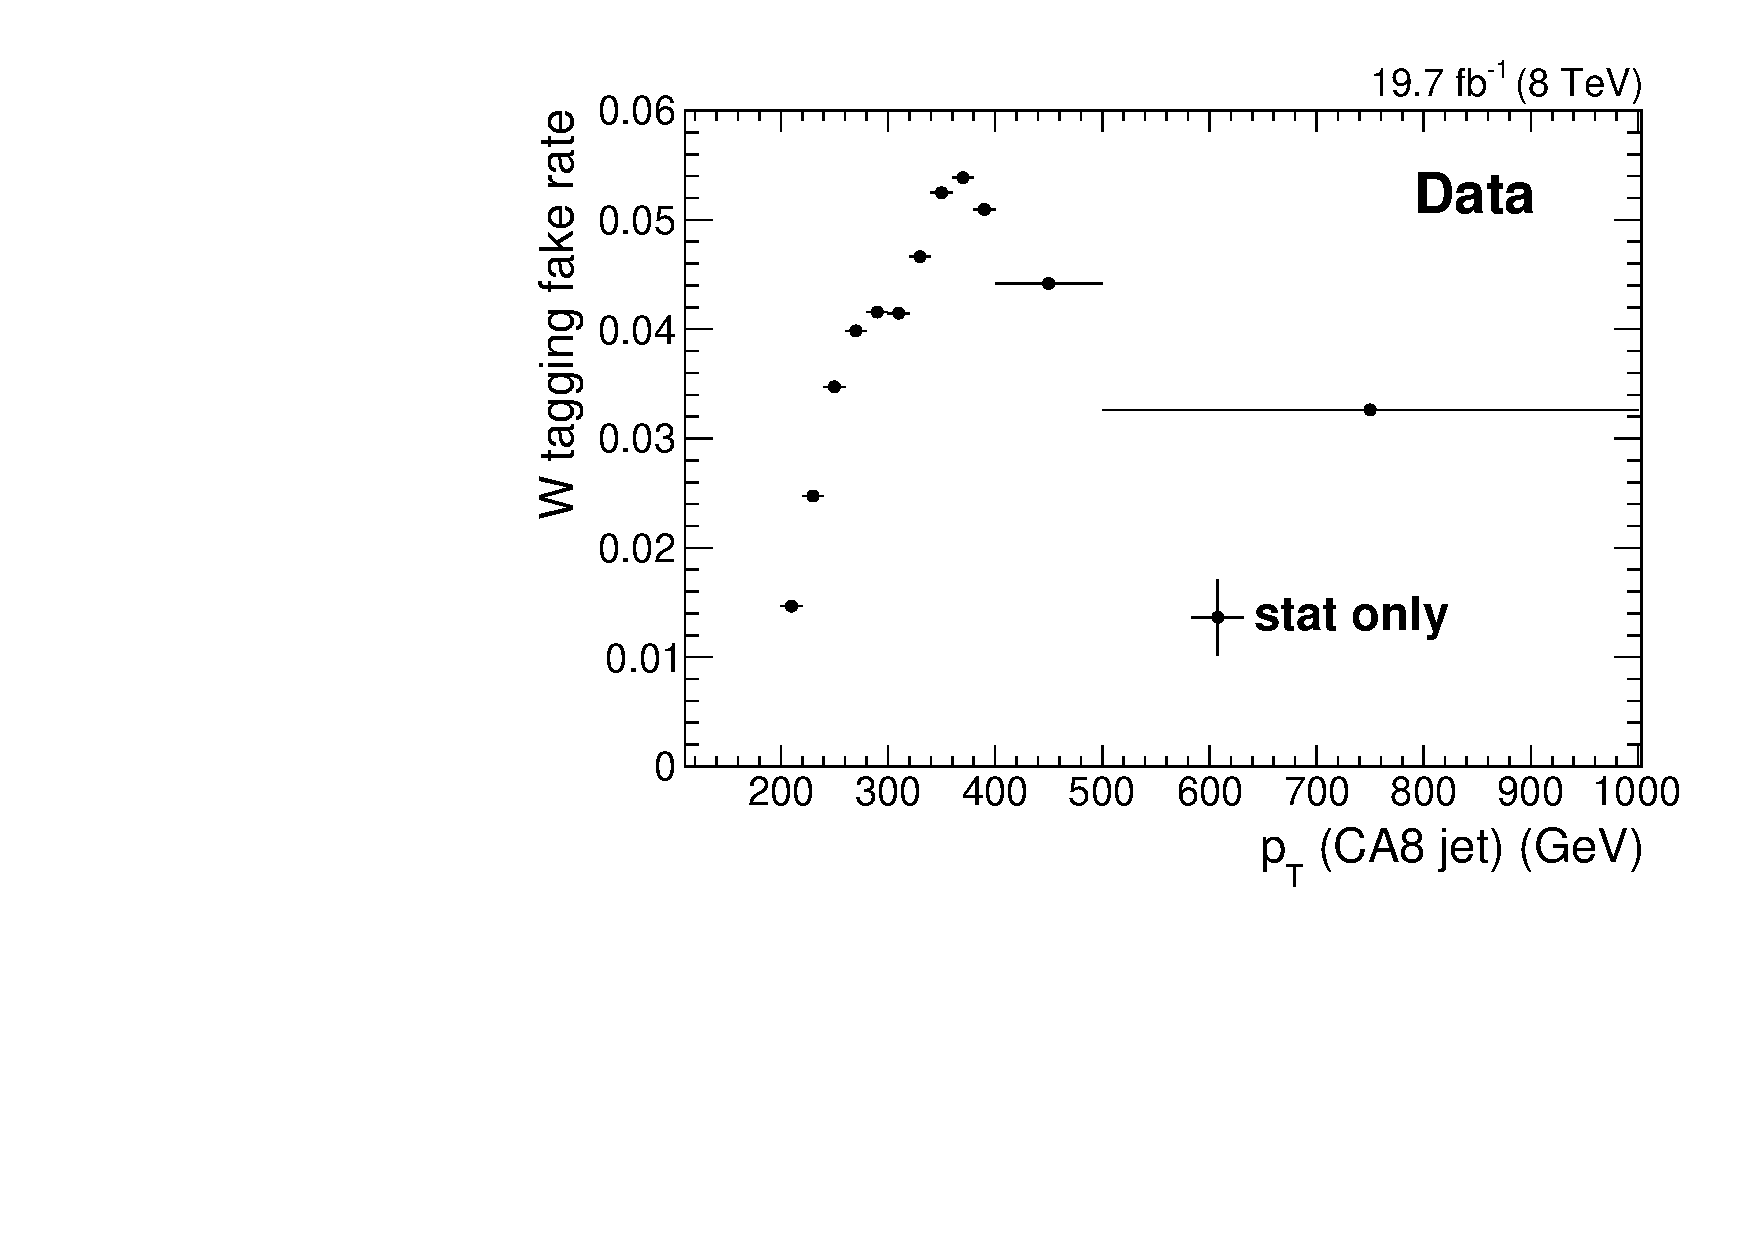
\includegraphics[width=0.6\textwidth]{figures/razor_wtag/Eff_Data_ratio_pt_tagged_all_Data_Thesis}

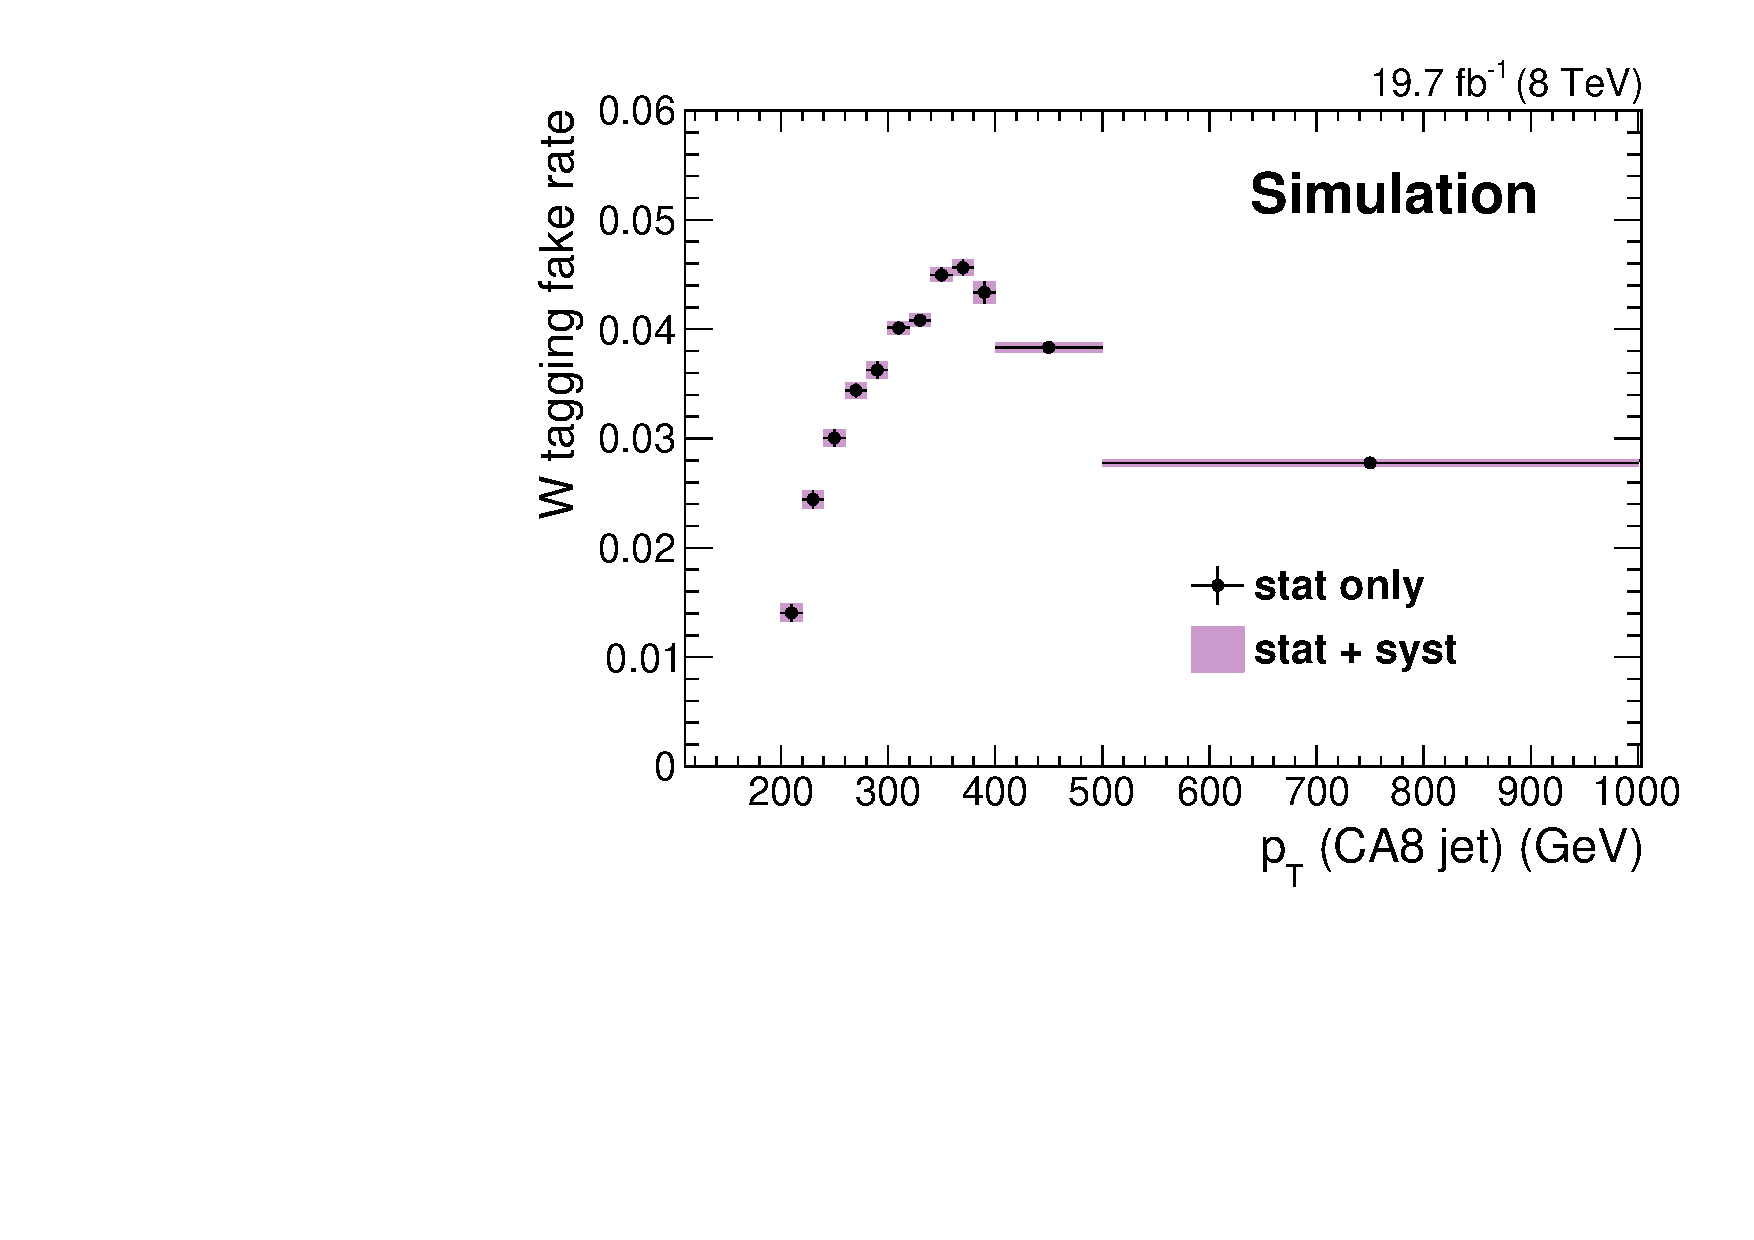
\includegraphics[width=0.6\textwidth]{figures/razor_wtag/Eff_MC_ratio_pt_tagged_all_MC_Thesis}

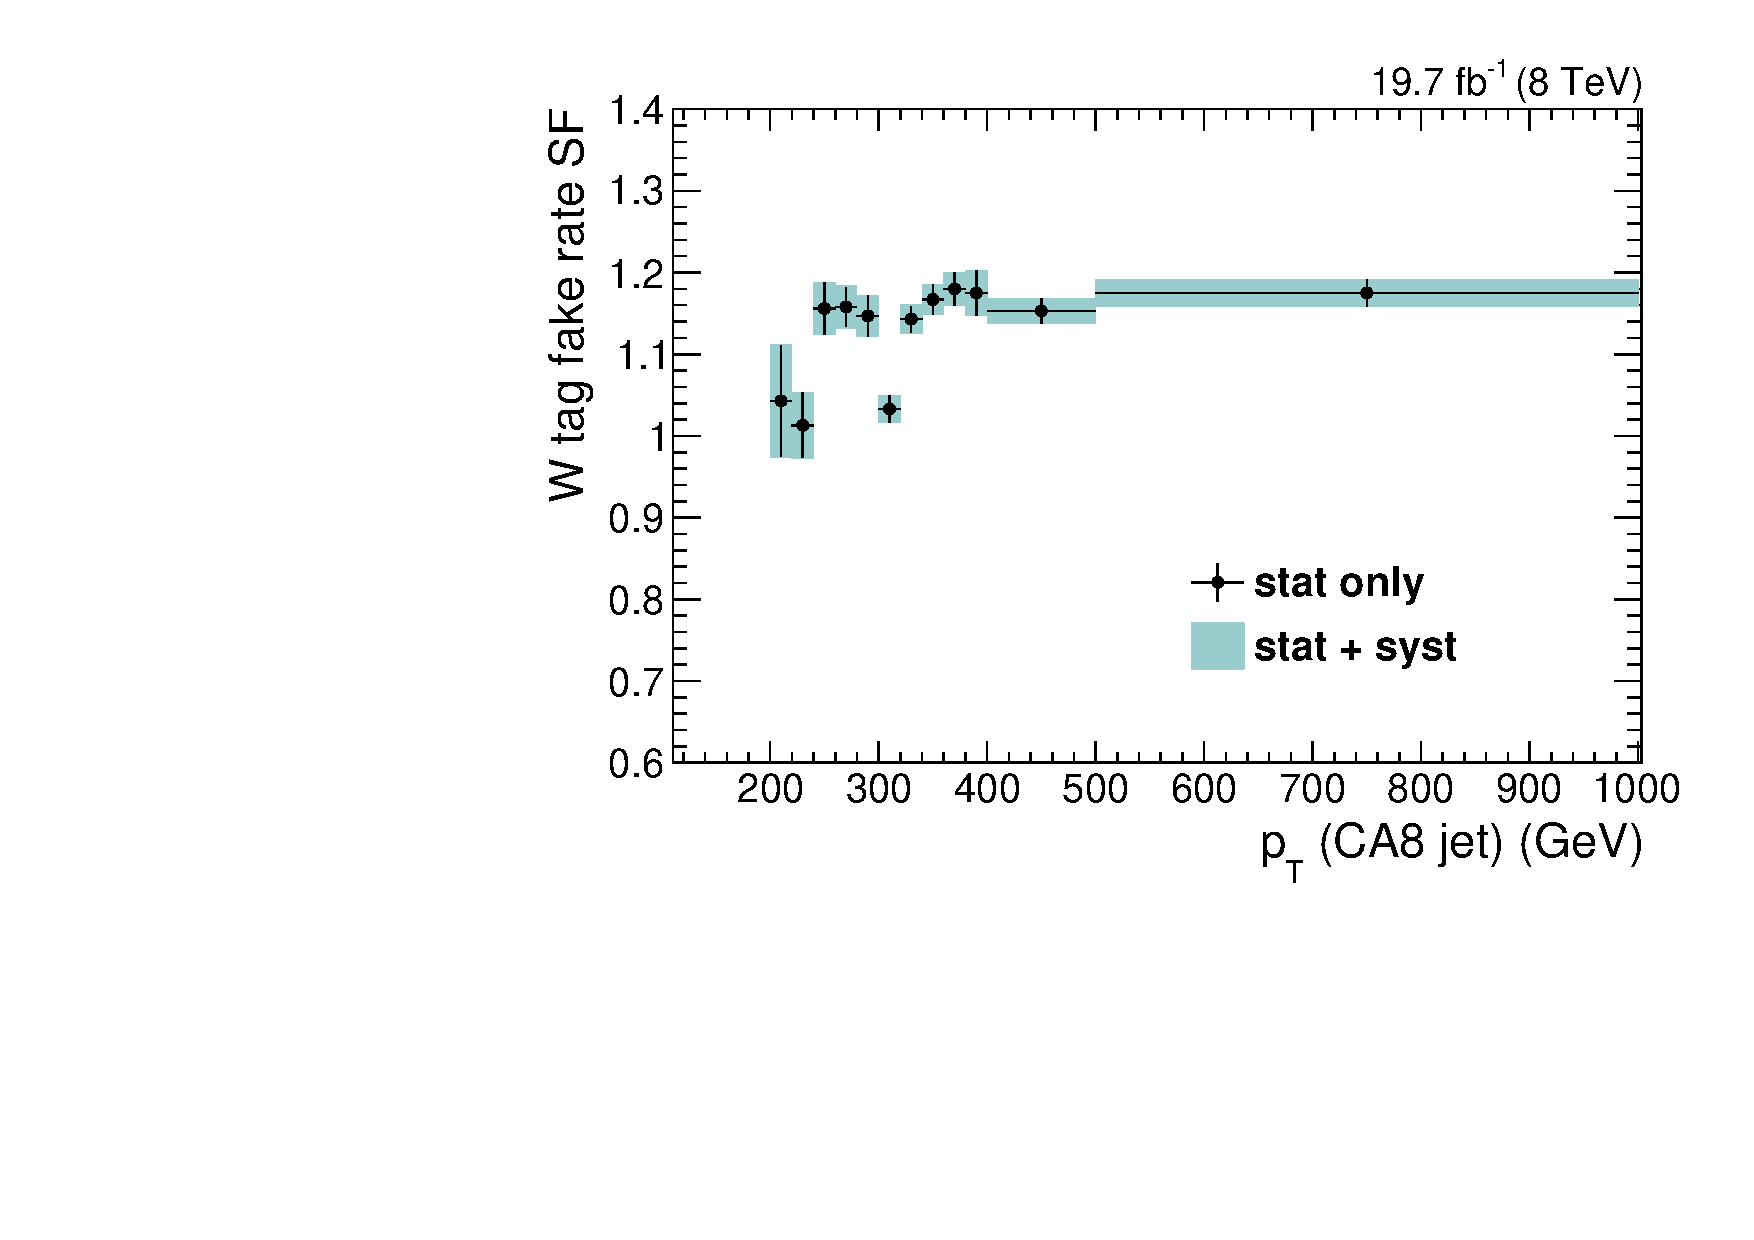
\includegraphics[width=0.6\textwidth]{figures/razor_wtag/SF_Wfake_Thesis}
\caption{[top] Misidentification probability according to $\W$ tagging for a CA8 jet versus
jet \pt obtained from a multijet-enriched control region in data as described in the text. The shown
uncertainties are statistical only. 
[middle] $\W$ boson tag fake rate obtained from simulation. The uncertainty band includes
statistical and systematic uncertainties.
[bottom] Scale factor for $\W$ tag fake rate versus CA8 jet \pt obtained from a
multijet-enriched control region as described in the text. The uncertainty band includes
statistical and systematic uncertainties.
\label{fig:boost_wfake}}
\end{figure}

The $\W$ boson tag fake rate scale factor is applied in the $S$ and $T$ region, as is the case for
the $\W$ boson tag efficiency scale factor. It is applied to all simulated samples without real
hadronically decaying $\W$ bosons, such as multijet production, $W(\rightarrow\ell\nu)$+jets,
$DY(\rightarrow\ell\ell)$+jets, et cetera. 

%% ---------------------------------------------------------------------------------------------

\subsubsection{\texorpdfstring{$\W$}{W} boson mass-tag fake rate scale factor
\label{sec:wmasstag_fake_sf}}

This scale factor corresponds to the $\W$ mass-tagging definition, which will be used in the $W$
control region. As we will see further, the $W$ region is dominated by leptonically decaying $\W$
bosons. The mass-tagged jet, therefore, originates from a quark or gluon jet, and is a
misidentified $\W$ boson jet. For this reason we will derive the scale factor for the $\W$ boson
mass-tag fake rate from the same multijet-enriched region as was used to derive the scale factor for
the $\W$ boson tag fake rate. The same method as before is applied, the only difference being
the use of the $\W$ boson mass-tag definition instead of the $\W$ boson tag definition. 

The resulting scale factor, $SF_\textrm{Wmasstag}^\textrm{fake}$, is again a function of the CA8
jet \pt, and will be applied to all simulated samples in the $W$ region.
Figure~\ref{fig:boost_wmasstag} shows the $\W$ boson mass-tag fake rate in data and
simulation, and the corresponding scale factor versus CA8 jet \pt. The scale factor is also
listed in Table~\ref{tab:SF_Wmass}. 
The drop in the scale factor just above a \pt of 300\GeV is also visible here. 

\begin{table}[htbp]
\centering
\caption{$\W$ boson mass-tag fake rate scale factor, binned in $\pt$. The breakdown in statistical
and systematic uncertainties is shown.  \label{tab:SF_Wmass}}
\vspace{1ex}
\begin{tabular}{c c}
\toprule
CA8 jet \pt (\GeV) & $SF_{\W\textrm{masstag}}^\textrm{fake}$ \\
\midrule
$[200 - 220[$ & $1.144 \pm 0.050 \,\textrm{(stat)} \pm 0.012 \,\textrm{(sys)}$ \\
$[220 - 240[$ & $1.118 \pm 0.028 \,\textrm{(stat)} \pm 0.024 \,\textrm{(sys)}$ \\
$[240 - 260[$ & $1.193 \pm 0.024 \,\textrm{(stat)} \pm 0.008 \,\textrm{(sys)}$ \\
$[260 - 280[$ & $1.250 \pm 0.018 \,\textrm{(stat)} \pm 0.015 \,\textrm{(sys)}$ \\
$[280 - 300[$ & $1.273 \pm 0.017 \,\textrm{(stat)} \pm 0.021 \,\textrm{(sys)}$ \\
$[300 - 320[$ & $1.126 \pm 0.013 \,\textrm{(stat)} \pm 0.010 \,\textrm{(sys)}$ \\
$[320 - 340[$ & $1.199 \pm 0.012 \,\textrm{(stat)} \pm 0.017 \,\textrm{(sys)}$ \\
$[340 - 360[$ & $1.298 \pm 0.013 \,\textrm{(stat)} \pm 0.007 \,\textrm{(sys)}$ \\
$[360 - 380[$ & $1.327 \pm 0.016 \,\textrm{(stat)} \pm 0.008 \,\textrm{(sys)}$ \\
$[380 - 400[$ & $1.339 \pm 0.025 \,\textrm{(stat)} \pm 0.007 \,\textrm{(sys)}$ \\
$[400 - 500[$ & $1.339 \pm 0.012 \,\textrm{(stat)} \pm 0.005 \,\textrm{(sys)}$ \\
$[500 - ...]$ & $1.370 \pm 0.011 \,\textrm{(stat)} \pm 0.001 \,\textrm{(sys)}$ \\
\bottomrule
\end{tabular}
\end{table}

\begin{figure}[htbp]
\centering
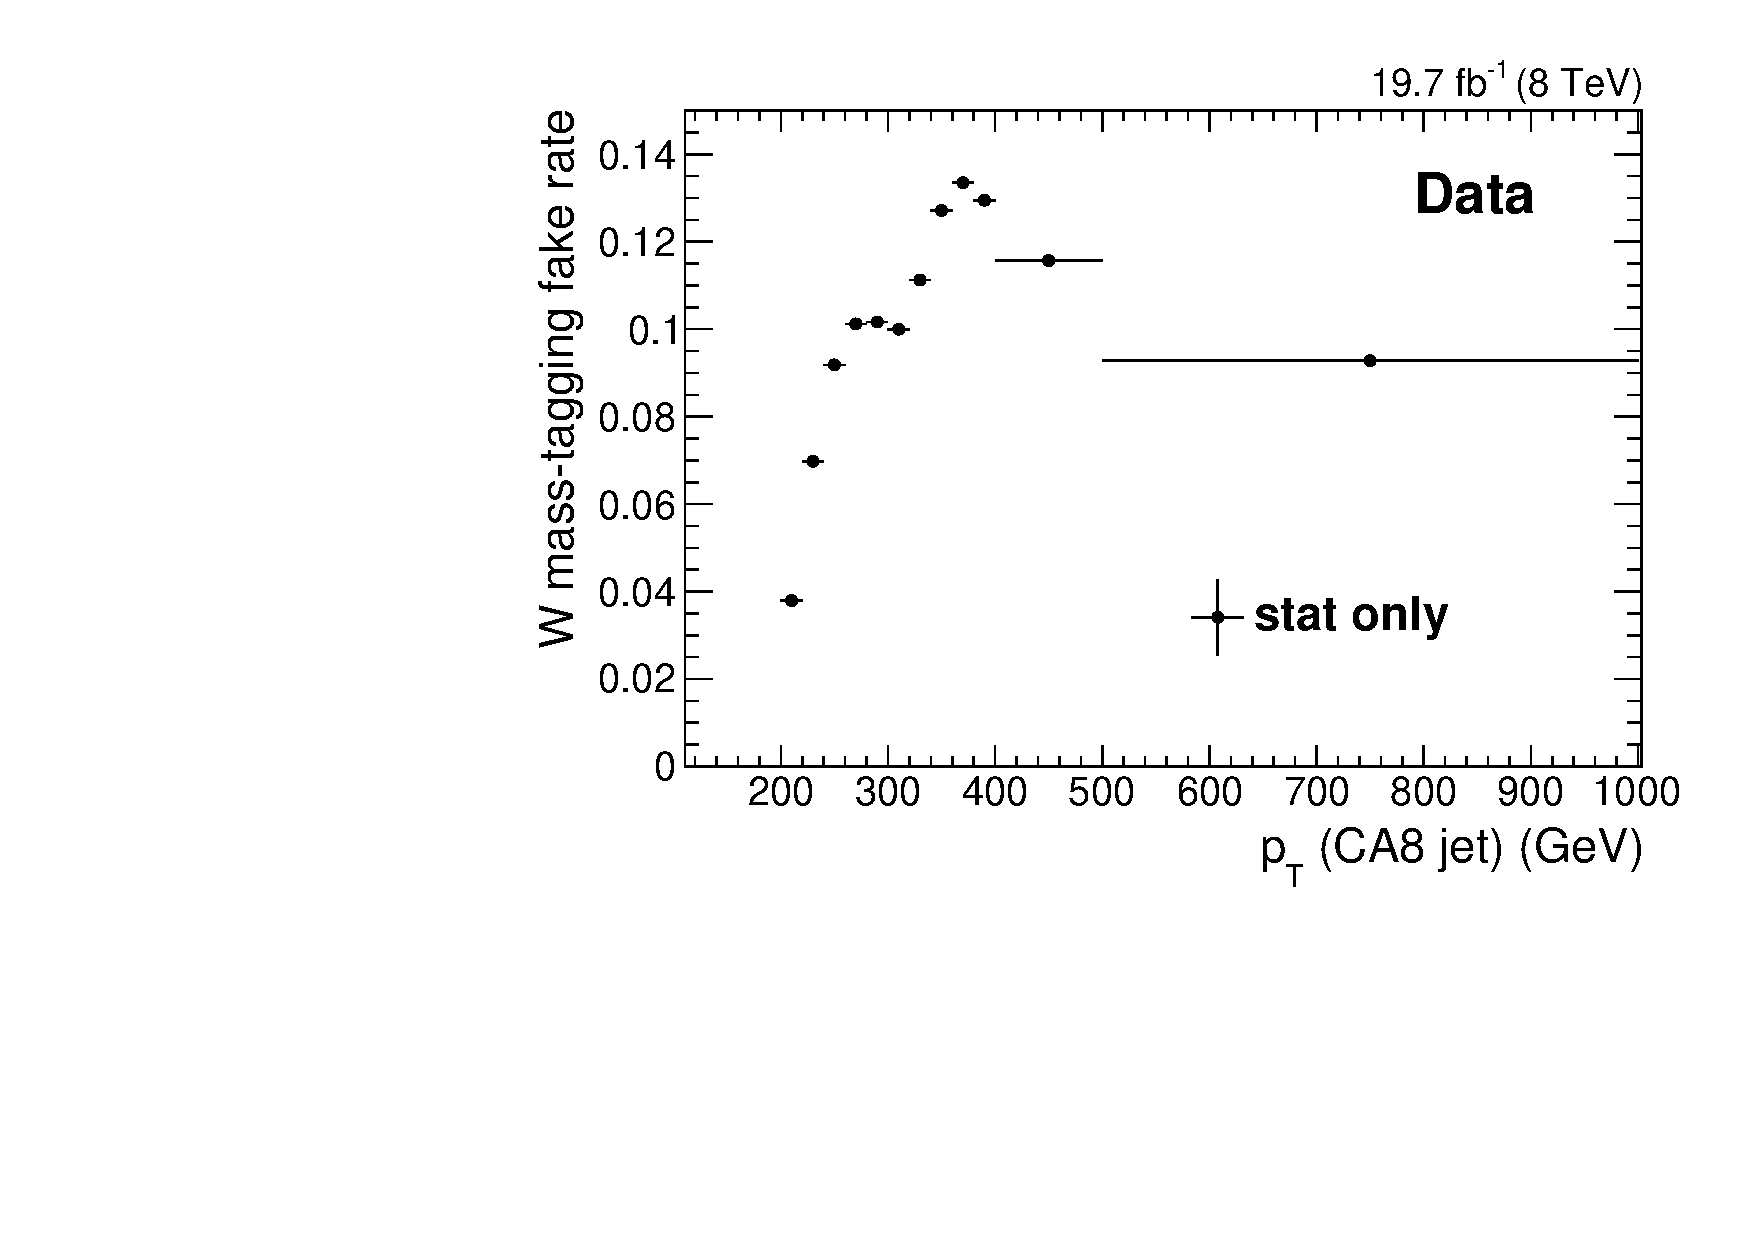
\includegraphics[width=0.6\textwidth]{figures/razor_wtag/Eff_Data_ratio_pt_Wmass_all_Data_Thesis}

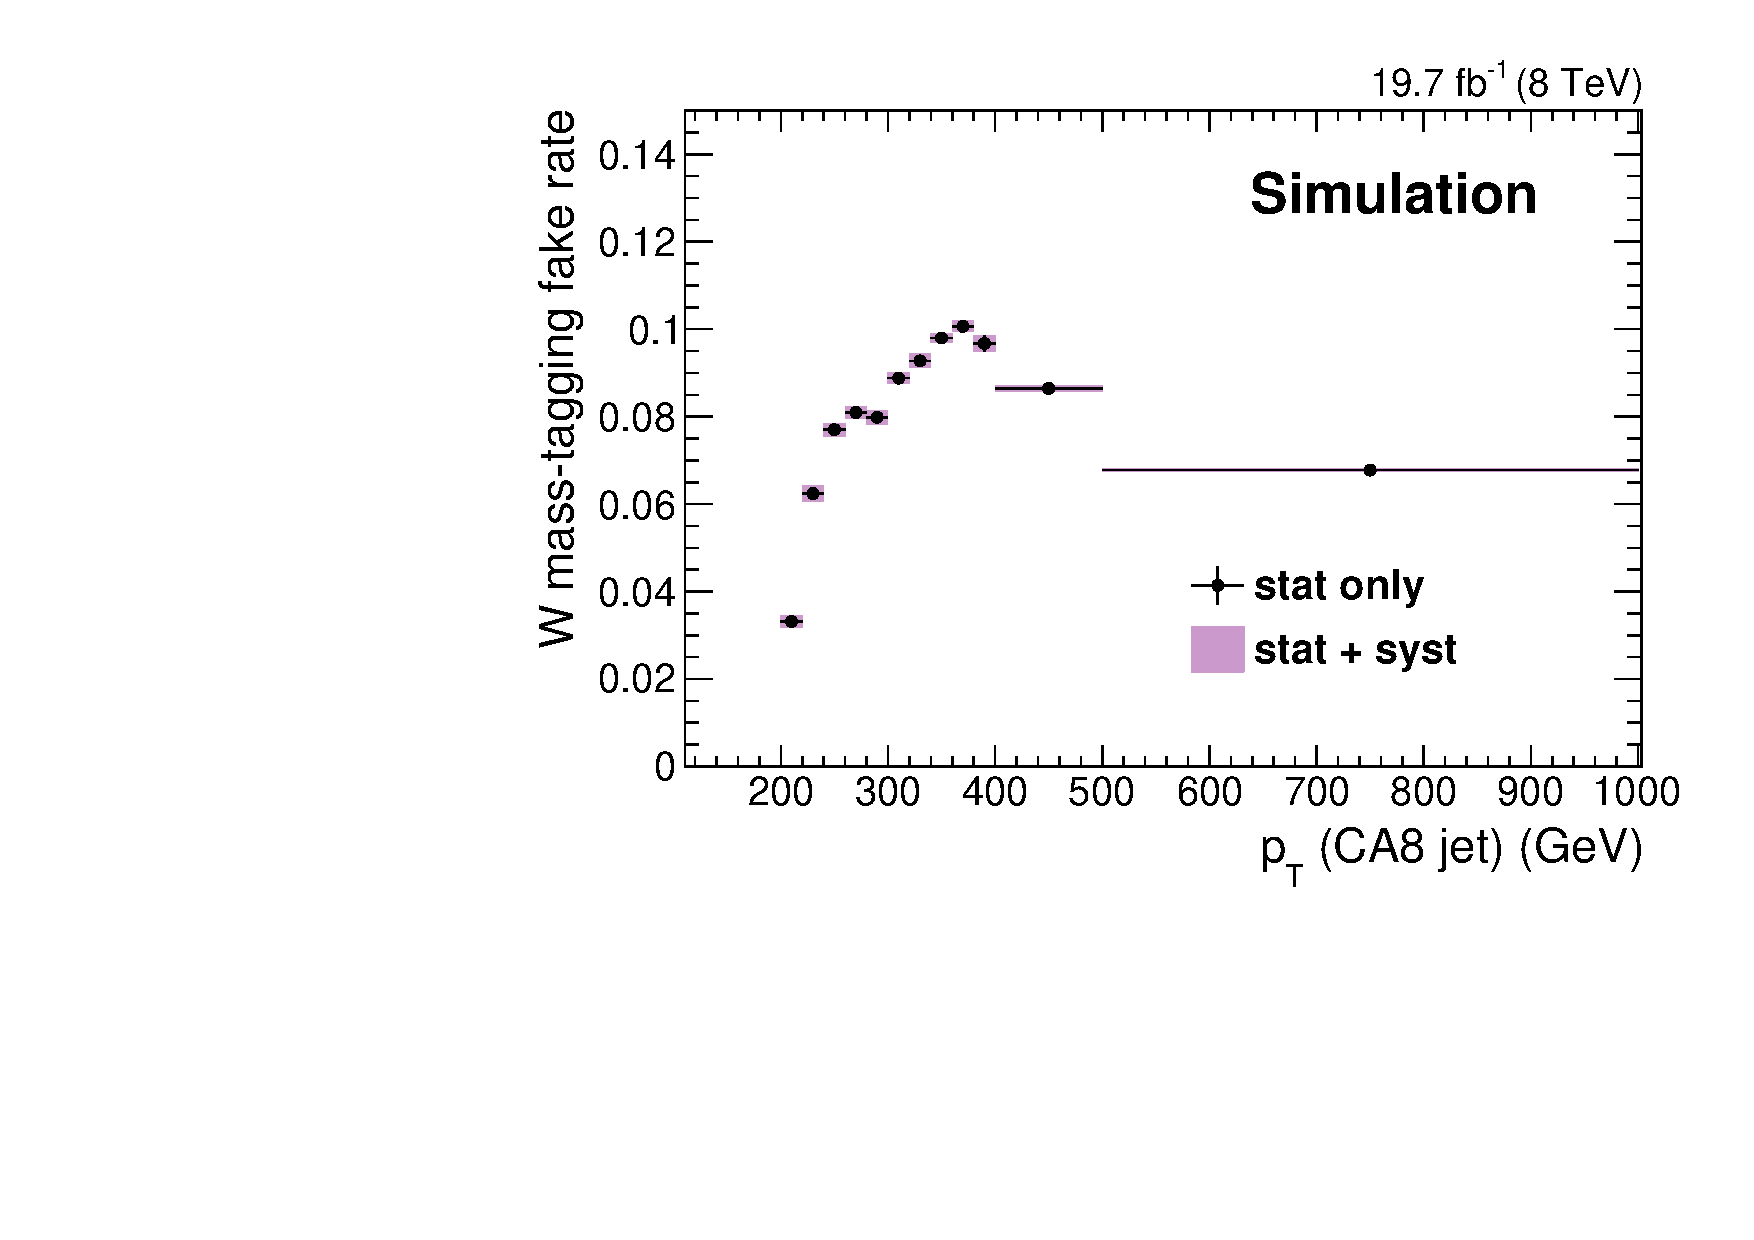
\includegraphics[width=0.6\textwidth]{figures/razor_wtag/Eff_MC_ratio_pt_Wmass_all_MC_Thesis}

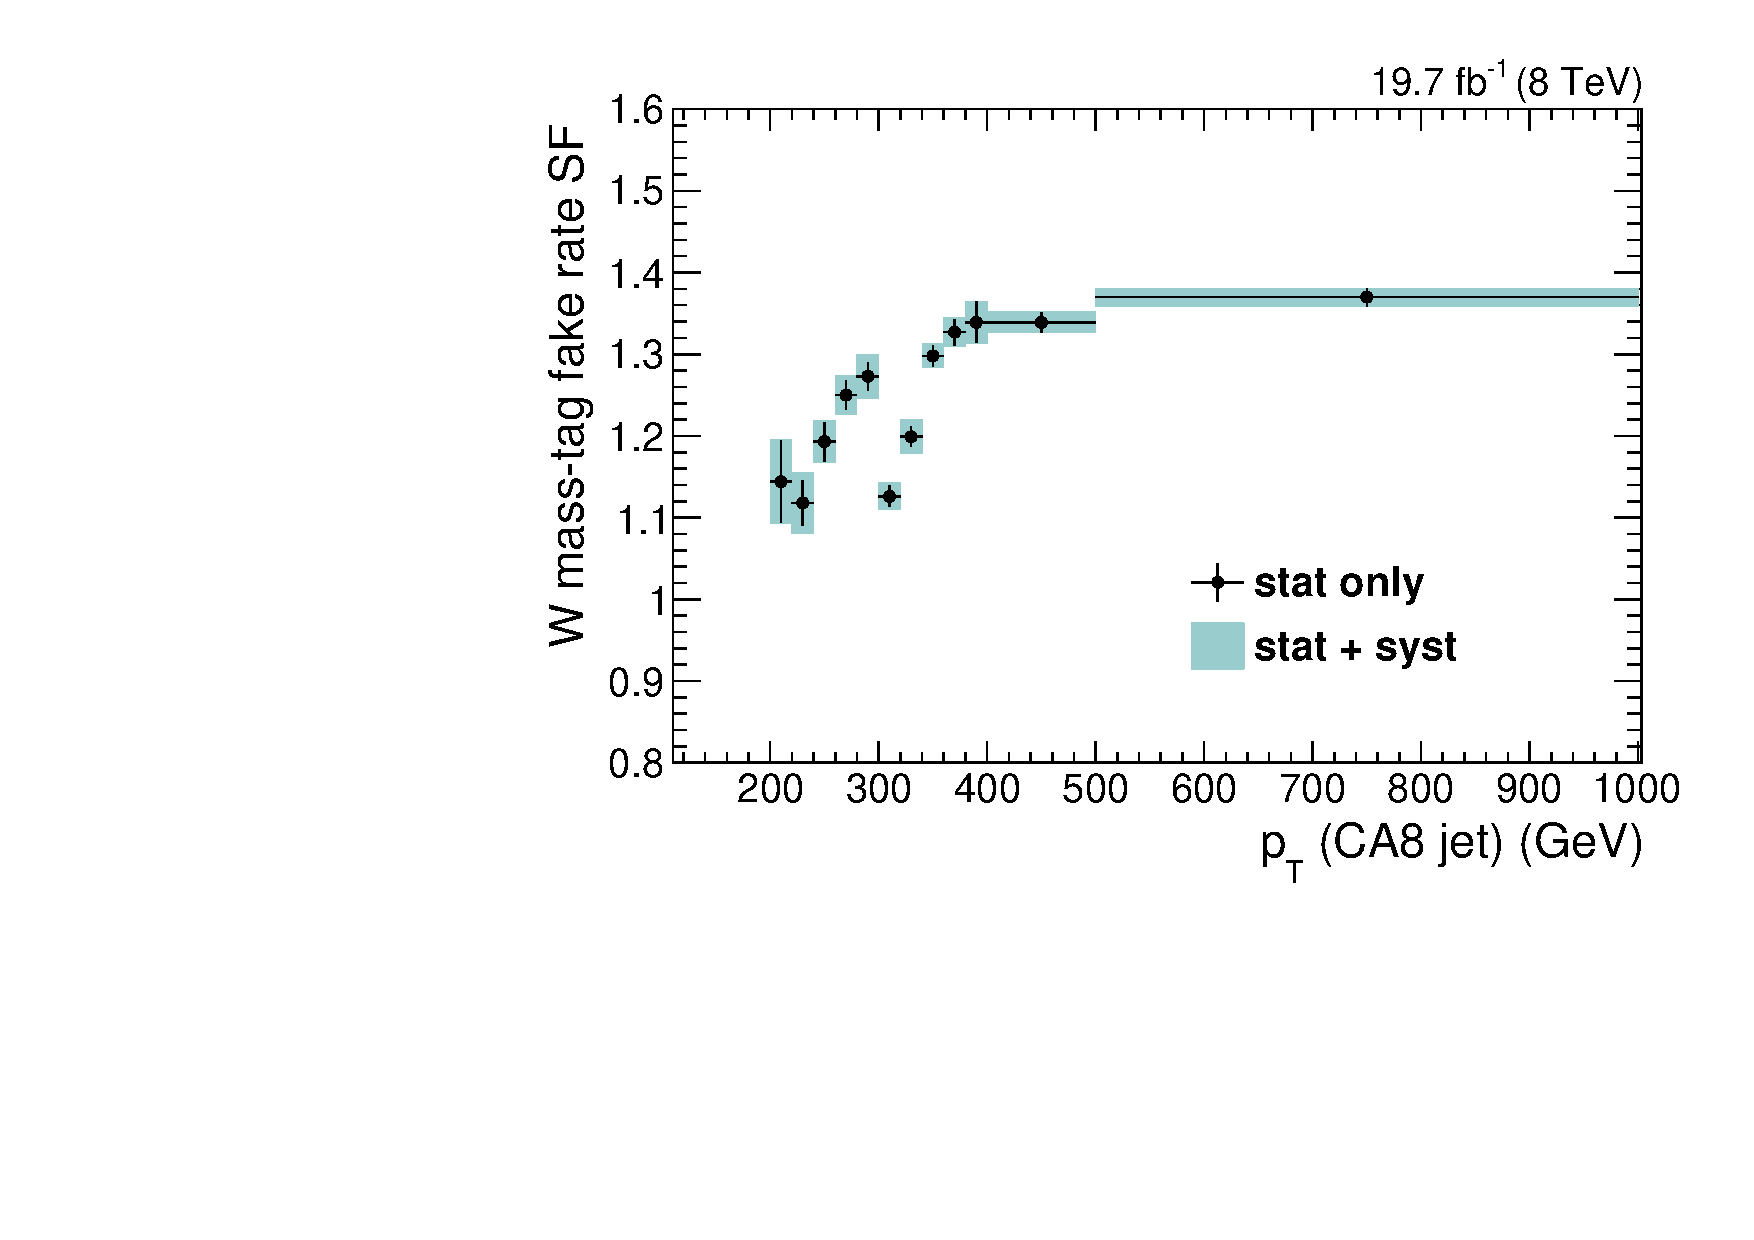
\includegraphics[width=0.6\textwidth]{figures/razor_wtag/SF_Wmass_Thesis}
\caption{[top] Misidentification probability according to $\W$ mass-tagging for a CA8 jet versus
jet \pt obtained from a multijet-enriched control region in data as described in the text. The shown
uncertainties are statistical only.
[middle] $\W$ boson mass-tag fake rate according to simulation. The uncertainty band includes
statistical and systematic uncertainties.
[bottom] Scale factor for $\W$ mass-tag fake rate versus CA8 jet \pt obtained from a
multijet-enriched control region as described in the text. The uncertainty band includes
statistical and systematic uncertainties.
\label{fig:boost_wmasstag}}
\end{figure}

%% ---------------------------------------------------------------------------------------------

\subsubsection{\texorpdfstring{$\W$}{W} boson anti-tag fake rate scale factor
\label{sec:wantitag_fake_sf}}

This scale factor corresponds to the $\W$ boson anti-tagging definition, which will be used in the
$Q$ control region. This region is dominated by QCD multijet production. Consequently, the $\W$
anti-tagged jet originates from a quark/gluon jet and is a misidentified $\W$ boson jet. Once
more, we use the same procedure and the multijet-enriched region as for the $\W$ boson tag fake
rate scale factor.

The $\W$ boson anti-tag fake rate scale factor, $SF_\textrm{Wantitag}^\textrm{fake}$, will be
applied to all simulated samples in the $Q$ region. 
Figure~\ref{fig:boost_wantitag} shows the $\W$ boson anti-tag fake rate in data and
simulation, and the corresponding scale factor versus CA8 jet \pt. As before, we observe a drop in
the scale factor just above a \pt of 300\GeV. The scale factor, and breakdown of statistical and
systematic uncertainties, is also listed in Table~\ref{tab:SF_Wantitagging}.


\begin{table}[htbp]
\centering
\caption{$\W$ boson anti-tag fake rate scale factor, binned in $\pt$. The uncertainties are broken
down in their statistical and systematic component. \label{tab:SF_Wantitagging}}
\vspace{1ex}
\begin{tabular}{c c}
\toprule
CA8 jet \pt $(\GeV)$ & $SF_{\W \textrm{antitag}}^\textrm{fake}$ \\
\midrule
$[200 - 220[$ & $1.217 \pm 0.072 \,\textrm{(stat)} \pm 0.032 \,\textrm{(sys)}$ \\
$[220 - 240[$ & $1.186 \pm 0.037 \,\textrm{(stat)} \pm 0.046 \,\textrm{(sys)}$ \\
$[240 - 260[$ & $1.216 \pm 0.033 \,\textrm{(stat)} \pm 0.011 \,\textrm{(sys)}$ \\
$[260 - 280[$ & $1.319 \pm 0.024 \,\textrm{(stat)} \pm 0.019 \,\textrm{(sys)}$ \\
$[280 - 300[$ & $1.479 \pm 0.022 \,\textrm{(stat)} \pm 0.037 \,\textrm{(sys)}$ \\
$[300 - 320[$ & $1.203 \pm 0.017 \,\textrm{(stat)} \pm 0.015 \,\textrm{(sys)}$ \\
$[320 - 340[$ & $1.244 \pm 0.016 \,\textrm{(stat)} \pm 0.026 \,\textrm{(sys)}$ \\
$[340 - 360[$ & $1.409 \pm 0.019 \,\textrm{(stat)} \pm 0.015 \,\textrm{(sys)}$ \\
$[360 - 380[$ & $1.448 \pm 0.022 \,\textrm{(stat)} \pm 0.020 \,\textrm{(sys)}$ \\
$[380 - 400[$ & $1.472 \pm 0.033 \,\textrm{(stat)} \pm 0.014 \,\textrm{(sys)}$ \\
$[400 - 500[$ & $1.487 \pm 0.017 \,\textrm{(stat)} \pm 0.012 \,\textrm{(sys)}$ \\
$[500 - ...]$ & $1.505 \pm 0.014 \,\textrm{(stat)} \pm 0.004 \,\textrm{(sys)}$ \\
\bottomrule
\end{tabular}
\end{table}


\begin{figure}[htbp]
\centering
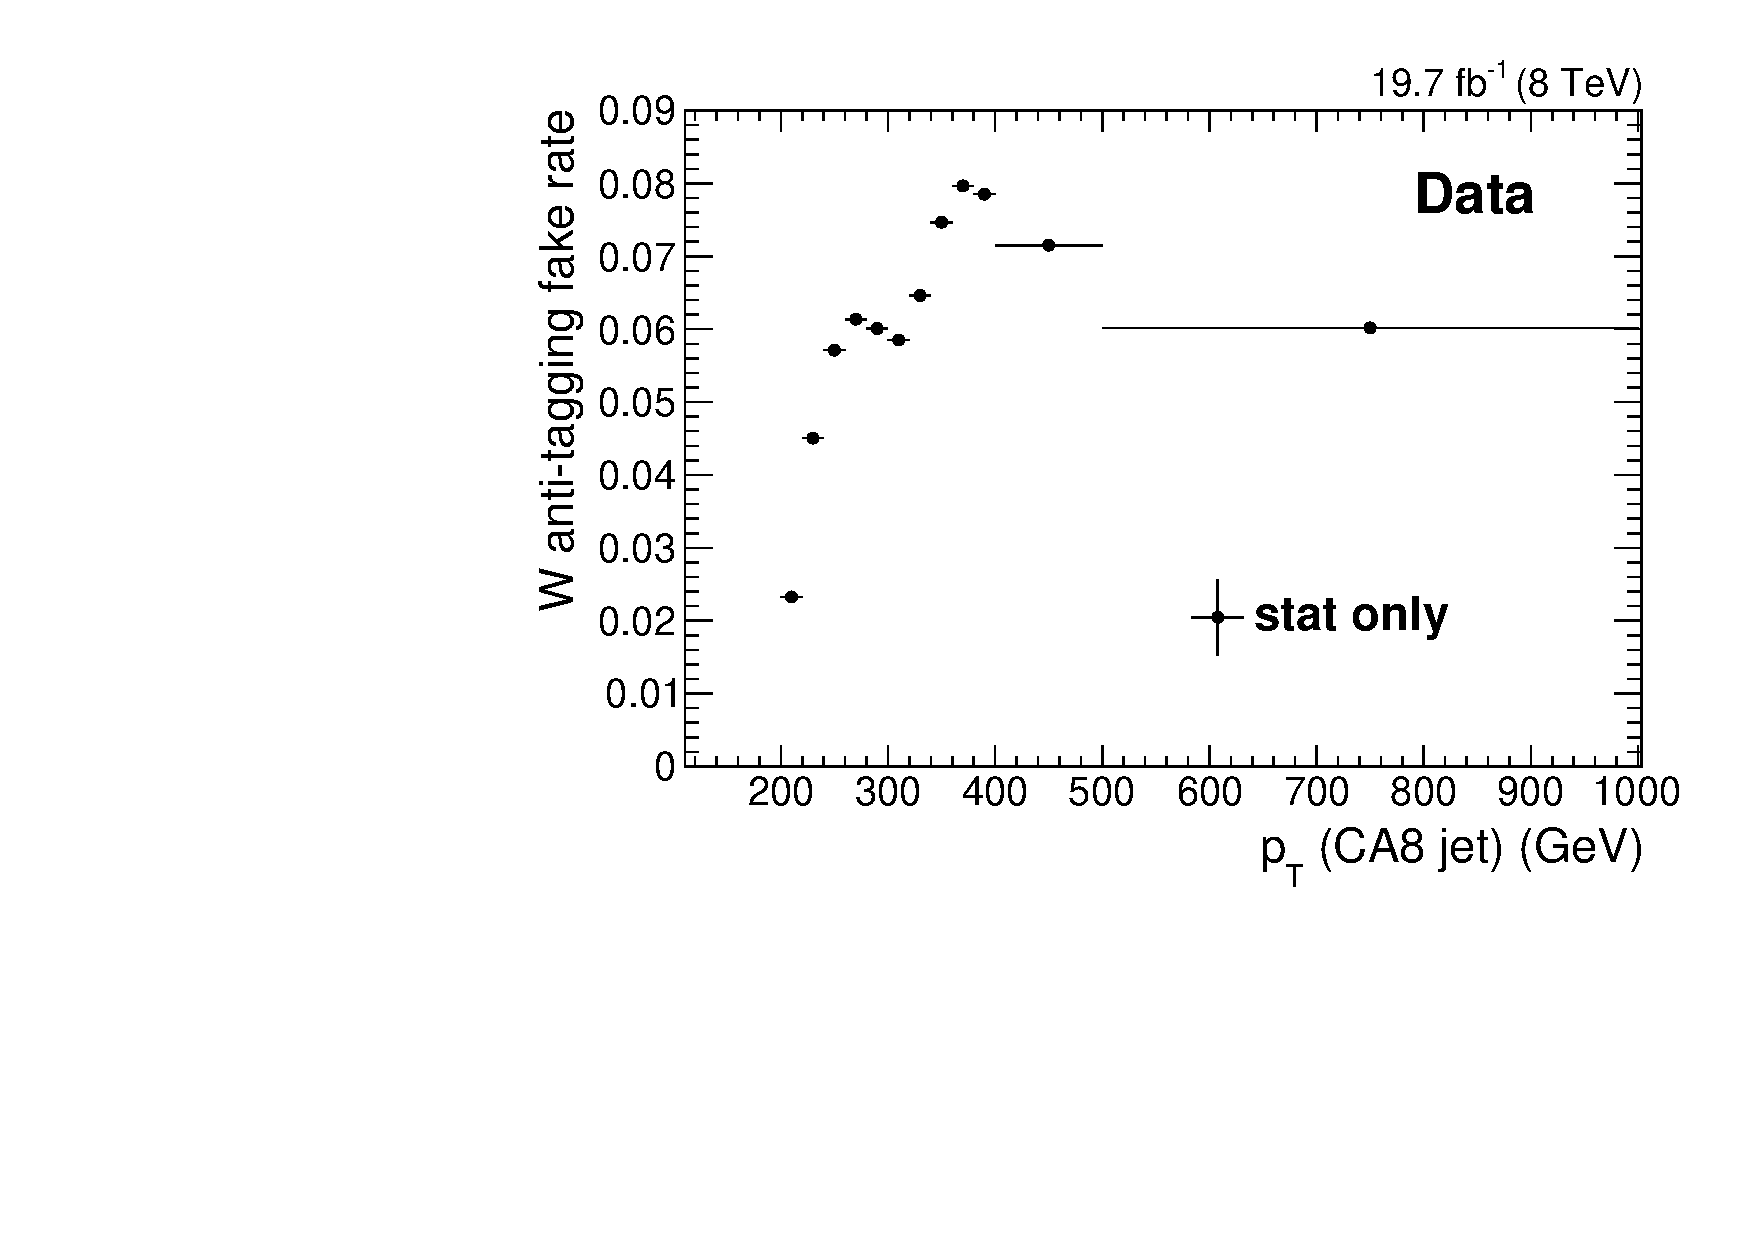
\includegraphics[width=0.6\textwidth]
{figures/razor_wtag/Eff_Data_ratio_pt_antitagged_all_Data_Thesis}

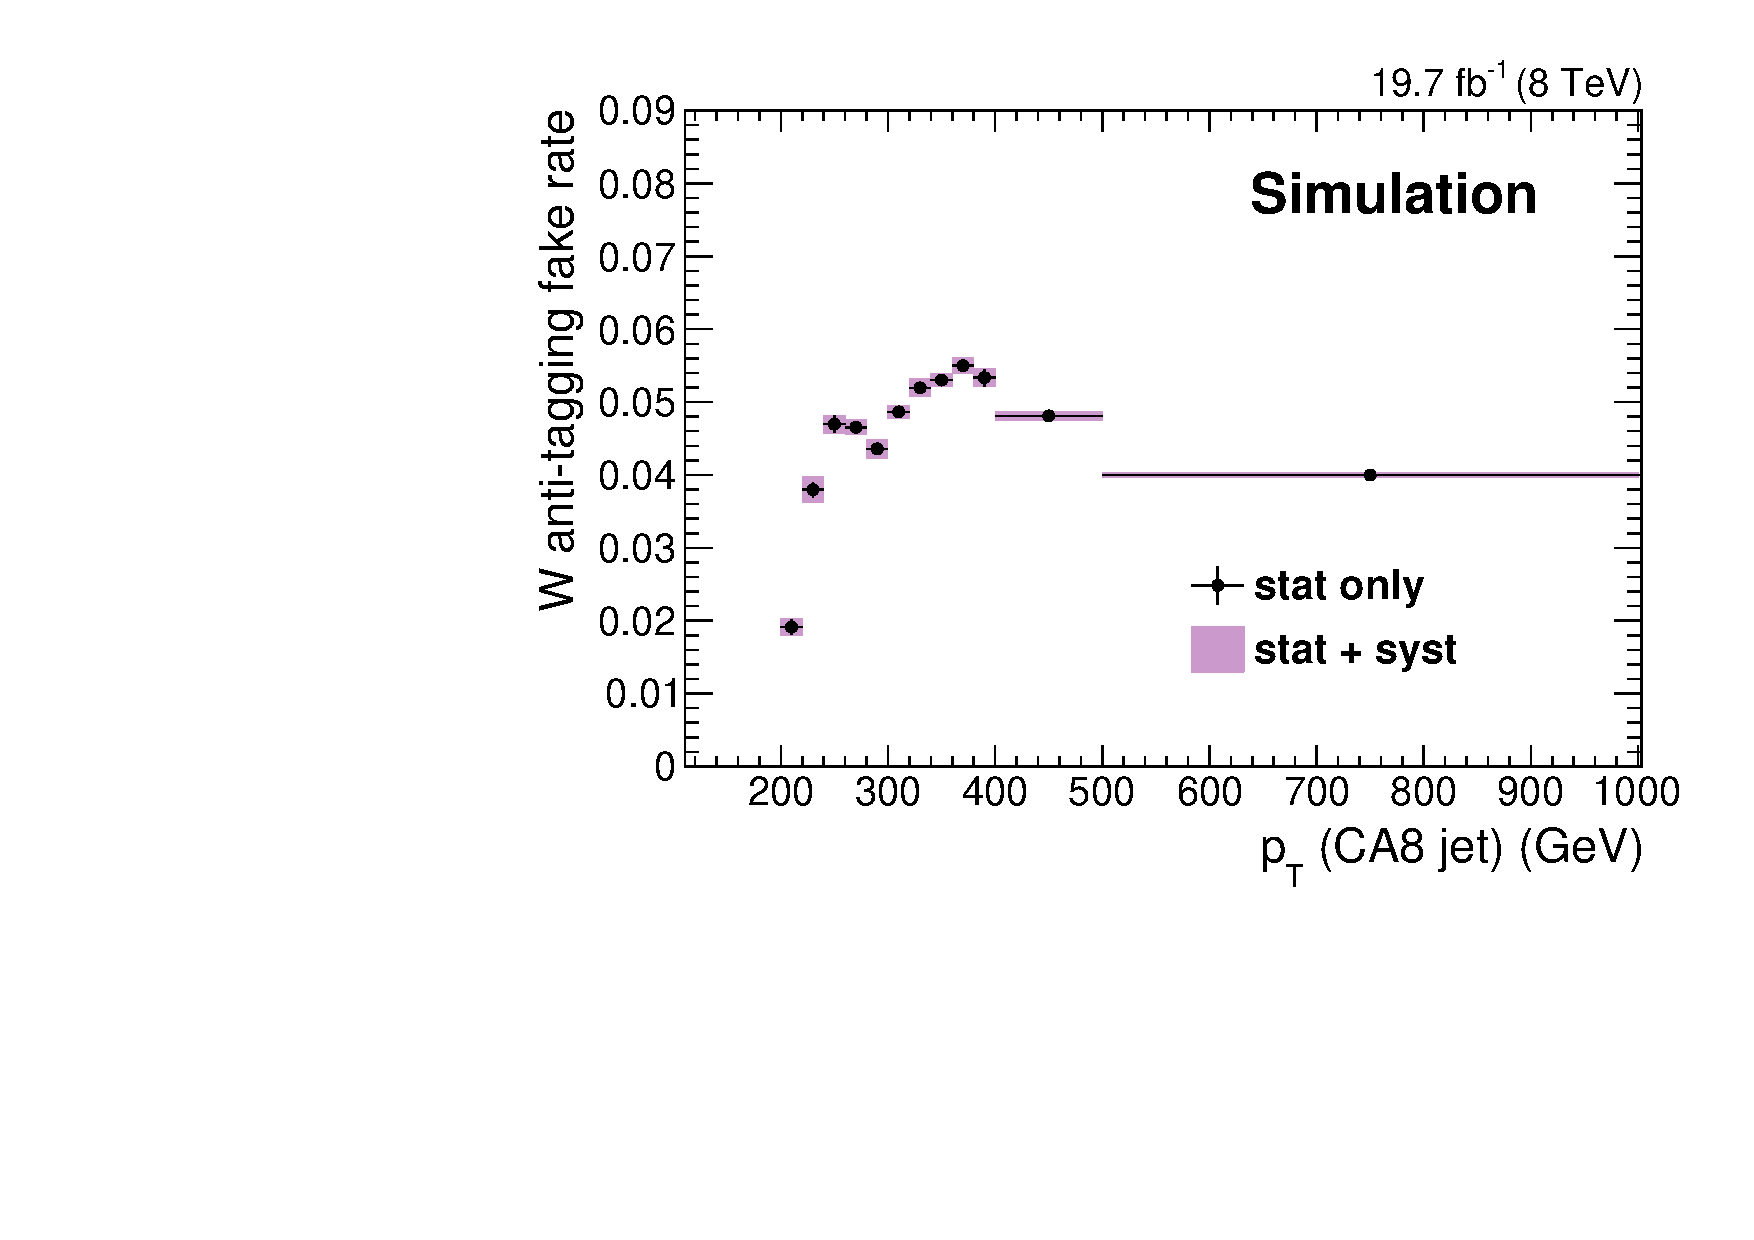
\includegraphics[width=0.6\textwidth]{figures/razor_wtag/Eff_MC_ratio_pt_antitagged_all_MC_Thesis}

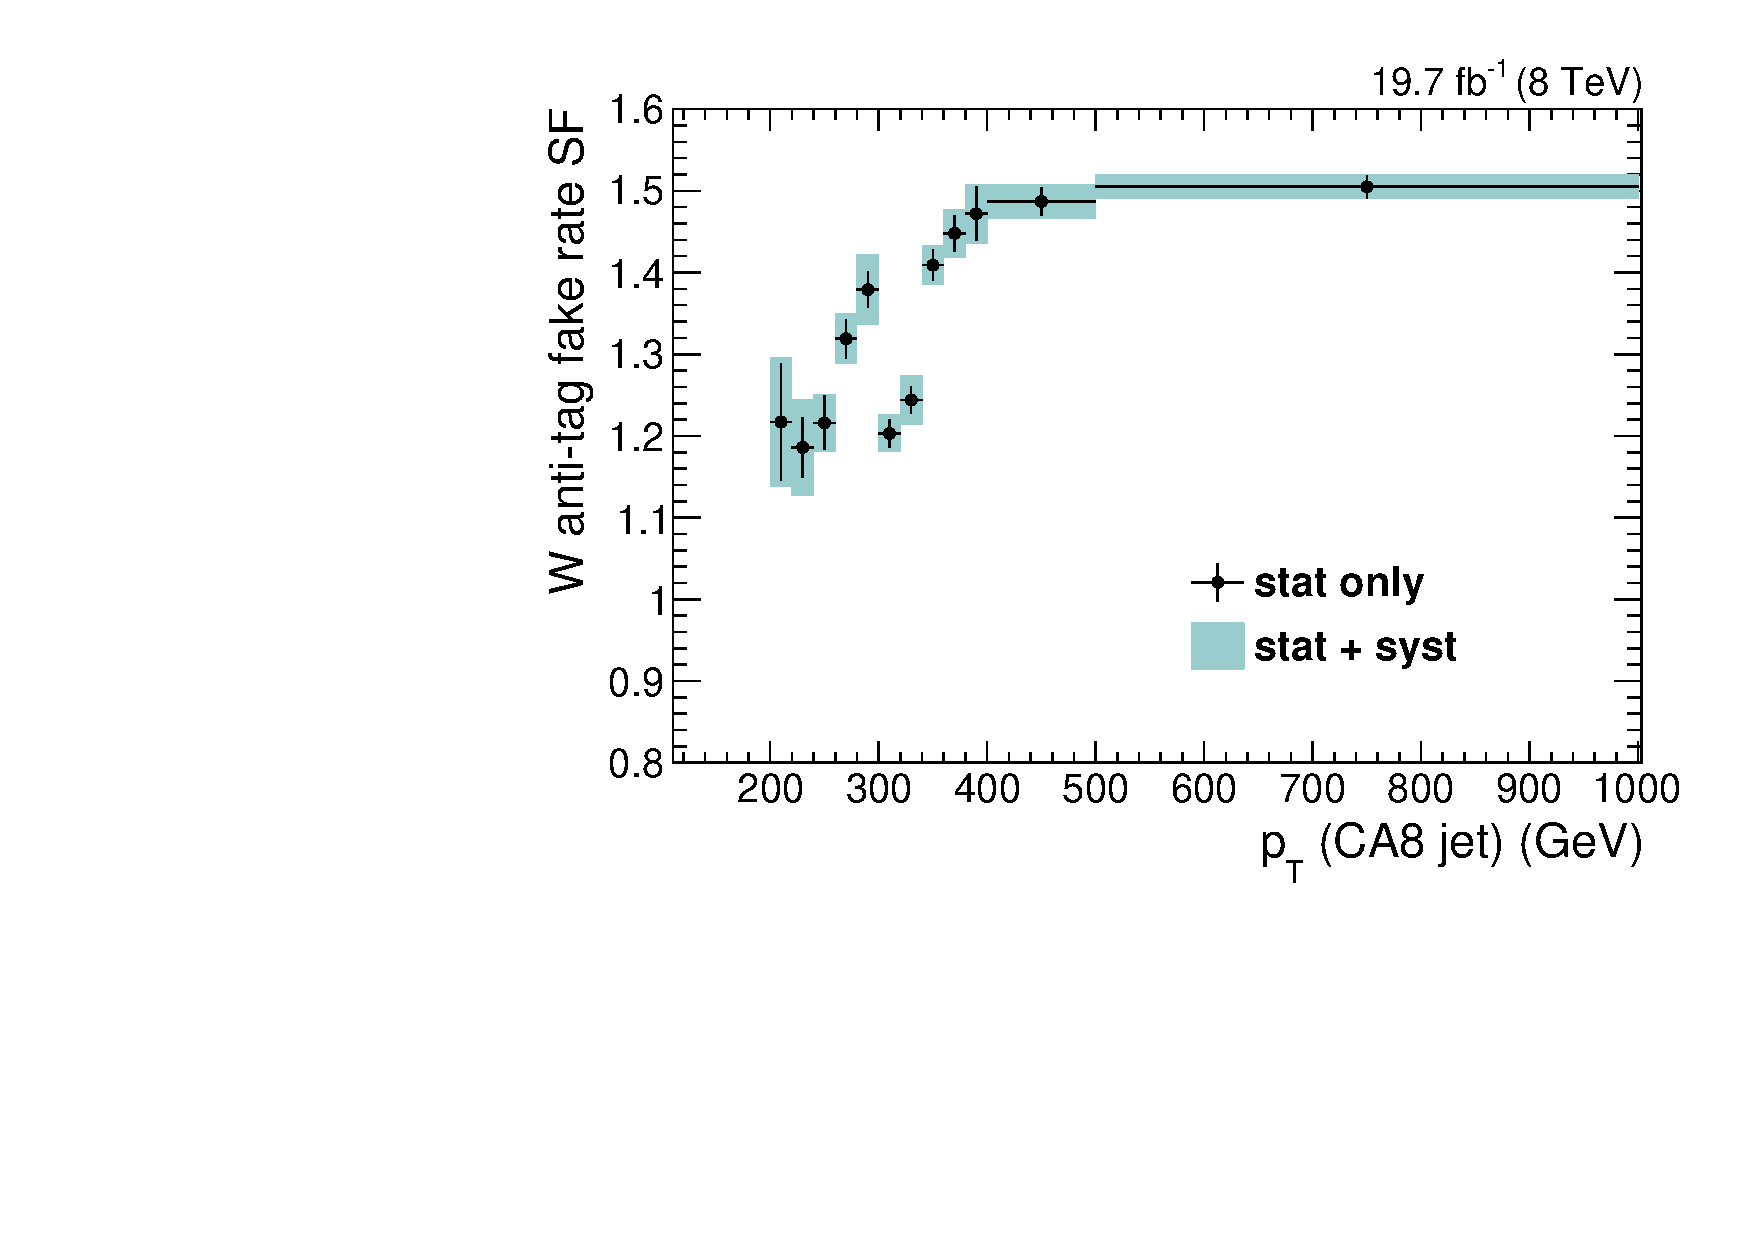
\includegraphics[width=0.6\textwidth]{figures/razor_wtag/SF_Wantitagged_Thesis}
\caption{[top] Misidentification probability according to $\W$ anti-tagging for a CA8 jet versus jet
\pt obtained from a multijet-enriched control region in data as described in the text. The shown
uncertainties are statistical only.
[middle] $\W$ boson anti-tag fake rate according to simulation. The uncertainty band includes
statistical and systematic uncertainties. 
[bottom] Scale factor for $\W$ anti-tag fake rate versus CA8 jet \pt obtained from a
multijet-enriched control region as described in the text. The uncertainty band includes
statistical and systematic uncertainties.
\label{fig:boost_wantitag}}
\end{figure}


% TODO explain the wiggle

%%%%%%%%%%%%%%%%%%%%%%%%%%%%%%%%%%%%%%%%%%%%%%%%%%%%%%%%%%%%%%%%%%%%%%%%%%%%%%%%%%%%%%%%%%%%%%%%%%%%



% 
% As we can see from these figures, there is a drop in the scale factor around a \pt of 300\GeV. 
% This is a result of a residual mismodeling of the trigger efficiency, as is explained in more detail
% in appendix~\ref{app:wiggle}. 
% Given that we understand the origin of this wiggle, we decide to keep the binning quite fine in that
% region, so that we can correct for the effect. 

\begin{table}[htbp]
\centering
\caption{Summary of scale factors and their total uncertainty. \label{tab:SF_summary}}
\vspace{1ex}
\begin{tabular}{c c c c}
\toprule
CA8 jet \pt (\GeV) & $SF_{\W\textrm{tag}}^\textrm{fake}$ & $SF_{\W \textrm{masstag}}^\textrm{fake}$
& $SF_{\W\textrm{antitag}}^\textrm{fake}$ \\
\midrule
$[200 - 220[$ & $1.04 \pm 0.07$ & $1.14 \pm 0.06$ & $1.22 \pm 0.08$ \\
$[220 - 240[$ & $1.01 \pm 0.04$ & $1.12 \pm 0.04$ & $1.19 \pm 0.06$ \\
$[240 - 260[$ & $1.16 \pm 0.04$ & $1.19 \pm 0.03$ & $1.22 \pm 0.04$ \\
$[260 - 280[$ & $1.16 \pm 0.03$ & $1.25 \pm 0.03$ & $1.32 \pm 0.04$ \\
$[280 - 300[$ & $1.15 \pm 0.03$ & $1.27 \pm 0.03$ & $1.38 \pm 0.05$ \\
$[300 - 320[$ & $1.03 \pm 0.02$ & $1.13 \pm 0.02$ & $1.20 \pm 0.03$ \\
$[320 - 340[$ & $1.14 \pm 0.02$ & $1.20 \pm 0.03$ & $1.24 \pm 0.03$ \\
$[340 - 360[$ & $1.17 \pm 0.02$ & $1.30 \pm 0.02$ & $1.41 \pm 0.03$ \\
$[360 - 380[$ & $1.18 \pm 0.03$ & $1.33 \pm 0.02$ & $1.45 \pm 0.03$ \\
$[380 - 400[$ & $1.18 \pm 0.03$ & $1.34 \pm 0.03$ & $1.47 \pm 0.04$ \\
$[400 - 500[$ & $1.15 \pm 0.02$ & $1.34 \pm 0.02$ & $1.49 \pm 0.03$ \\
$[500 - ...]$ & $1.18 \pm 0.02$ & $1.37 \pm 0.02$ & $1.51 \pm 0.02$ \\
\bottomrule
\end{tabular}
\end{table}



